\chapter{BaseLib Level 0}
\chaptermark{Level 0}



BaseLib Level0 is a mixture of different classes that must provide the developer with a complete system abstraction. In fact such abstraction stops at the operating system level without offering device driver's API. Each device driver must be developed separately for a specific architecture and OS. \\

To better understand what services there are in BaseLib Level 0 the following argomentation subdivid it in a logical way extrapolating these sections:

\begin{itemize}
 \item Architectures
 \item Lists

 \item IPC

 \item Network
 \item Files, Streams

 \item Errors, Exceptions
 \item Memory
 \item Processes, Threads

 \item Mathematic
\end{itemize}

BaseLib2 was already ported to the following OS: OS/2$^{\copyright}$, VxWorks$^{\copyright}$, Linux, Linux/RTAI, Solaris$^\copyright$ and MS Windows$^\copyright$.






\section{Architectures}
\begin{figure}[h!]
 \begin{center}
  \includegraphics[width=\textwidth]{level0/level0-arch.eps}
  \caption{BaseLib Level0 Architecture classes}
  \label{f:level0:arch}
 \end{center}
\end{figure}

This group of classes (Figure \ref{f:level0:arch}) adds the very low level support to the library, addressing architecture and hardware support, i.e. processor assembly instructions and special processor register functions.
The Architecture group include the following classes:
\begin{itemize}
 \item Processor
 \item ProcessorType

 \item LoadableLibrary
 \item RTAILoader

 \item Atomic
 \item SPAtomic

 \item HRT (High Resolution Timer) 
 \item TimeoutType
 \item Sleep
\end{itemize}



\subsubsection{Processor}
\texttt{[Processor.h, Processor.cpp]}\\
The Processor class lets you discover how many processor there are on the machine and which kind of processor are and it's characteristics like the clock and the family name.

\begin{lstlisting}[
extendedchars=true,%
basicstyle=\fontfamily{pcr}\fontseries{m}\selectfont\footnotesize, %
stepnumber=1,%
numberstyle=\tiny,%
keywordstyle=\footnotesize\tt ,%
language=C++]
public:
   static uint64 ClockFrequency();
   static double ClockPeriod();

   static const char *Name();
   static uint32 Family();
   static uint32 Characteristic(uint32 capId);

   static int32 Available();
   static void ReScanCPU();
\end{lstlisting}

All methods are static; \texttt{ClockFrequency} return the CPU or the HRT frequency, \texttt{ClockPeriod} return the CPU period (the inverse of the frequency). \texttt{Name} return the processor name or type, \texttt{Family} return the brand of the processor, \texttt{Characteristic} return some capabilities of the CPU, \texttt{Available} return the number of available cpus on the system.
Th function \texttt{ReScanCPU} reinitialize the static processor object and redo a scan of the system to count the number of CPU.\\


In \textit{Processor.cpp} there is also a \texttt{HRTCalibrator} class that calibrate the CPU clock. Such class has only a constructor and no other methods or attributes. The \texttt{HRTCalibrator} class is statically instantiated with the name \texttt{hrtCalibrator}; it just sets some global variables at the start up executing the code in its contructor. \\



\subsubsection{ProcessorType}
\texttt{[ProcessorType.h]}\\
The \texttt{ProcessorType} class defines the processors where a particular task should run. There is a unique mask argument as a \texttt{uint32}, the \texttt{processorMask}, this is a bitmask and allow the maximum presence of 32 CPU on a system.
The interface let the user initialize the class with a bitmask and adding CPUs but never remove one or more. There are some operator overlaoding.


For example, if we have a task is that will run on cpu 2 and 3 the mask is: 0x06 (00000110).


\begin{lstlisting}[
extendedchars=true,%
basicstyle=\fontfamily{pcr}\fontseries{m}\selectfont\footnotesize, %
stepnumber=1,%
numberstyle=\tiny,%
keywordstyle=\footnotesize\tt ,%
language=C++]
public:
   uint32 processorMask;

   ProcessorType(const uint32 cpuMask = 0xFE);
   ProcessorType(const ProcessorType &pt);

   void SetMask(const uint32 mask);
   void AddCPU(const uint32 cpuNumber);

   void operator=(const uint32 cpuMask);
   void operator=(const ProcessorType &pt);
   void operator|=(const uint32 cpuMask);
   void operator|=(const ProcessorType &pt);
\end{lstlisting}



\subsubsection{LoadableLibrary}
\texttt{[LoadableLibrary.h]}\\
The class \texttt{LoadableLibrary} lets BaseLib, that is a component oriented framework, load its components by means of loading external libraries. On different Operating Systems libraries have different extensions.

\begin{table}[!h]
 \begin{center}
  \begin{tabular}{|l|l|}
   \hline
    GENERAL ACQUISITION MODULE & \texttt{*.gam} \\
    HIGH LEVEL DRIVER & \texttt{*.drv} \\
    STD NAME FOR DLL & \texttt{*.dll} \\
    LINUX NAME FOR DLL & \texttt{*.so} \\
   \hline
   \end{tabular}
   \end{center}
  \caption{Loadable libraries extensions}
 \label{t:extensions}
\end{table}



\subsubsection{Atomic}
\texttt{[Atomic.h, Atomic.cpp]}\\
The class is build up only of static methods. Such routines are performed by the CPU without interruption; these are slower than those in \textit{SPAtomic.h}, but are granted to work on multiprocessor machines.

The Solaris port is quite old and is the only one that is not coded with assembly instructions.

\begin{lstlisting}[
extendedchars=true,%
basicstyle=\fontfamily{pcr}\fontseries{m}\selectfont\footnotesize, %
stepnumber=1,%
numberstyle=\tiny,%
keywordstyle=\footnotesize\tt ,%
language=C++]
public:
   static inline void Increment (volatile int32 *p );
   static inline void Increment (volatile int16 *p);
   static inline void Increment (volatile int8 *p);

   static inline void Decrement (volatile int32 *p);
   static inline void Decrement (volatile int16 *p);
   static inline void Decrement (volatile int8 *p);

   static inline int32 Exchange (volatile int32 *p, int32 v);

   static inline bool TestAndSet(int32 volatile *p);
   static inline bool TestAndSet(int16 volatile *p);
   static inline bool TestAndSet(int8  volatile *p);
\end{lstlisting}

The class offer methods to atomically increment, decrement, exchange (swap) and test and set 8bit, 16bit and 32bit variables, 64bit variables are not supported yet.



\subsubsection{SPAtomic}
\texttt{[SPAtomic.h, SPAtomic.cpp]}\\
Single Processor Atomic operation support. The interface of exported methods is identical to the \texttt{Atomic} class, the only thing that differ is the source code: atomic operations are inherently processor dependent, not all CPU implements atomic instruction in the same way protecting sections to be exectued concurrently.\\ 


This routine are not processor safe, not to be executed in multiprocessor environments. \\


\begin{lstlisting}[
extendedchars=true,%
basicstyle=\fontfamily{pcr}\fontseries{m}\selectfont\footnotesize, %
stepnumber=1,%
numberstyle=\tiny,%
keywordstyle=\footnotesize\tt ,%
language=C++]
public:
    static inline void Increment (volatile int32 *p );
    static inline void Increment (volatile int16 *p);
    static inline void Increment (volatile int8 *p);

    static inline void Decrement (volatile int32 *p);
    static inline void Decrement (volatile int16 *p);
    static inline void Decrement (volatile int8 *p);

    static inline int32 Exchange (volatile int32 *p, int32 v);

    static inline bool TestAndSet(int32 volatile *p);
    static inline bool TestAndSet(int16 volatile *p);
    static inline bool TestAndSet(int8  volatile *p);
\end{lstlisting}



\subsubsection{HRT}
\texttt{[HRT.h, HRT.cpp]}\\
The HRT or High Resolution Timer class exhibit a series of public static methods. Methods let the user query the system High Resolution Timer about the current time count, in machine ticks. In a Pentium class processor the offered methods (\texttt{HRTCounter}, \texttt{HRTCounter32}) are perform a \texttt{rdtsc} assembly instruction respectively returning a 64bit and a 32bit number. The \texttt{rdtsc} x86 assembly instruction read the Time Stamp Counter register of the processor that is a 64bit register present on all x86 processors since the Pentium. It counts the number of ticks since reset.

\begin{lstlisting}[
extendedchars=true,%
basicstyle=\fontfamily{pcr}\fontseries{m}\selectfont\footnotesize, %
stepnumber=1,%
numberstyle=\tiny,%
keywordstyle=\footnotesize\tt ,%
language=C++]
public:
   static inline int64 HRTCounter();
   static inline uint32 HRTCounter32();
\end{lstlisting}

To convert the readed value to a more significant value there are some other methods. The method \texttt{HRTFrequency} return the CPU frequency, \texttt{HRTPeriod} the period of the CPU clock and \texttt{TicksToTime} simply convert CPU ticks in time (seconds).

\begin{lstlisting}[
extendedchars=true,%
basicstyle=\fontfamily{pcr}\fontseries{m}\selectfont\footnotesize, %
stepnumber=1,%
numberstyle=\tiny,%
keywordstyle=\footnotesize\tt ,%
language=C++]
   static inline int64 HRTFrequency();
   static inline double HRTPeriod();
   static inline double TicksToTime(int64 tStop,int64 tStart=0);

   uint32 SystemMsecTime();
\end{lstlisting}

Last method is not static and require an object to be instantiated. Is really strange that this method is static, looking at the implementation it doesn't require object attributes. It count the ms from reset.



\subsection{Design Notes}

HRT's last method must be static. Infact no class methods and attributes are called. The current code follow.

\begin{lstlisting}[
extendedchars=true,%
basicstyle=\fontfamily{pcr}\fontseries{m}\selectfont\footnotesize, %
stepnumber=1,%
numberstyle=\tiny,%
keywordstyle=\footnotesize\tt ,%
language=C++]
uint32 HRTSystemMsecTime(){
   int64 count      =  HRTRead64();
   double msecTime  =  HRTClockCycle() * 1000.0;
   msecTime = msecTime * count;
   return (uint32) msecTime;
}
\end{lstlisting}

\texttt{HRTCalibrator} class must be moved and integrated in \texttt{HRT} class; now it is declared in Processor.cpp, not well designed. \\


ProcessorType class is not scalable. Scalability and modularity are central concepts of Object Oriented Design. It is not a good choice to dress a \texttt{uint32} as a class with only one real method (\texttt{Add}). The first step is to add at least a \texttt{Remove} method. The second step is to extend the \texttt{ProcessorType} class to support a generic number of processors; instead of an uint32 we have to add a bitmap, in this way we can define a set of class that work on bitmaps and support a generic number of processors.\\


Another required extension (that could be handle in a generic way) is the support of atomic operation with generic length variables starting with the 64bit support in the \texttt{Atomic} and \texttt{SPAtomic} classes. \\






\section{Lists}
\begin{figure}[h!]
 \begin{center}
  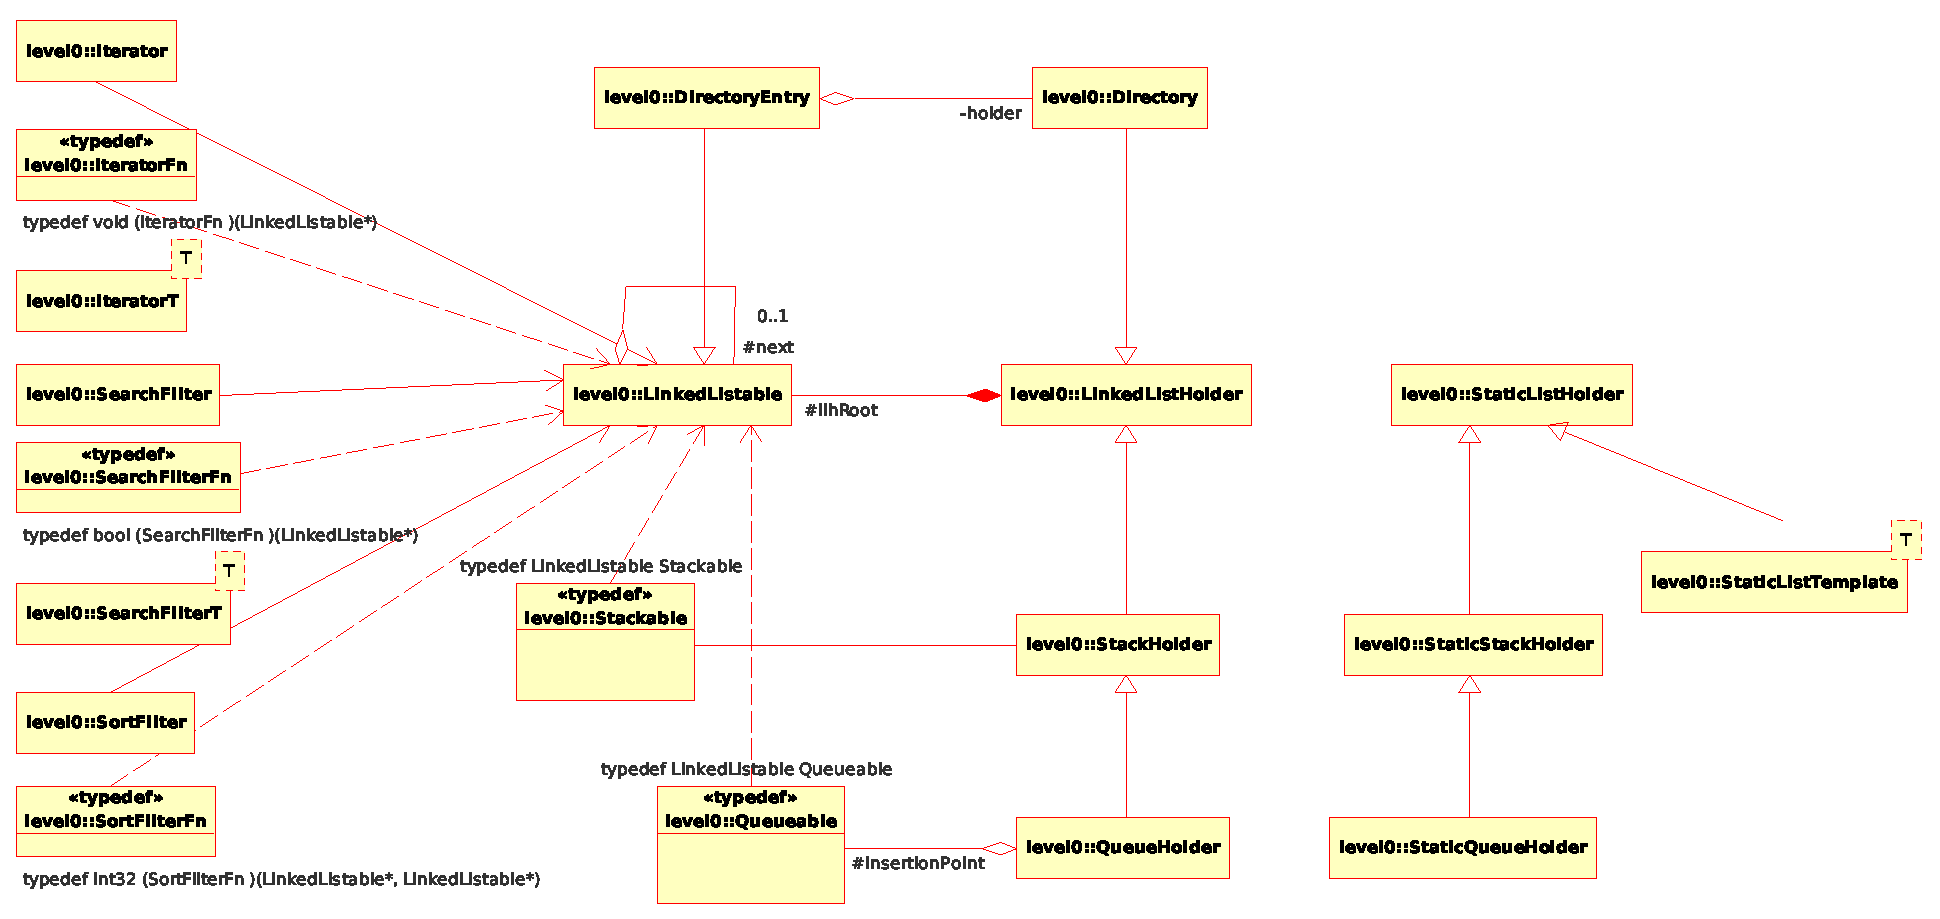
\includegraphics[width=\textwidth]{level0/level0-lists.eps}
  \caption{BaseLib Level0 Lists classes}
  \label{f:level0:lists}
 \end{center}
\end{figure}

The list abstraction is the most used abstraction in BaseLib. On top of a linked list it's build each BaseLib's DataBase; the SemNameDataBase (SNDB), GlobalObjectDataBase (GODB), ObjectRegistryDataBase (ORDB), ConfigurationDataBase (CDB) and many others.

Lists are mainly divided in two categories: linked list and static list. Figure \ref{f:level0:lists} graph all classes involved in this group, those classes can be further splitted in linked and static list and an the \textit{directory} abstraction that is a simple implementation of a single linked list. Static lists are basically vectors.



\subsection{Linked Lists}
\begin{figure}[h!]
 \begin{center}
  \includegraphics[width=\textwidth]{level0/level0-linked.eps}
  \caption{BaseLib Level0 Linked Lists classes}
  \label{f:level0:linked}
 \end{center}
\end{figure}

Figure \ref{f:level0:linked} depict classes involved in the linked list abstraction offered in BaseLib, the \texttt{directory} abstraction is not presented again. The basic building block of a linked list is a \texttt{LinkedListable} element that is typedefined to became a \texttt{Stackable} and a \texttt{Queueable} object, but is still the same. The modules that you are going to explore are:

\begin{itemize}
 \item LinkedListable

 \item LinkedListHolder
 \item StackHolder
 \item QueueHolder

 \item Iterator, IteratorT, IteratorFn
 \item SearchFilter, SearchFilterT, SearchFilterFn
 \item SortFilter, SortFilterFn
\end{itemize}

Still in this section we discuss about the \texttt{Directory} example that let you puts the hands on the BaseLib \textit{LinkedList} interface.

\begin{itemize}
 \item DirectoryEntry
 \item Directory
\end{itemize}



\subsubsection{LinkedListable}
\texttt{[LinkedListable.h]}\\
 A linked list member. Can be used as root of a linked list, a specific linked list member can be derived from this class (so can be subclassed). The \texttt{LinkedListable} interface must be subclassed to became specific.

A \texttt{LinkedListable} object holds only a pointer to the next \texttt{LinkedListable} object.

\begin{lstlisting}[
extendedchars=true,%
basicstyle=\fontfamily{pcr}\fontseries{m}\selectfont\footnotesize, %
stepnumber=1,%
numberstyle=\tiny,%
keywordstyle=\footnotesize\tt ,%
language=C++]
protected:
   LinkedListable *next;
\end{lstlisting}

The \texttt{Next} method return the pointer to the next \texttt{LinkedListable} object; while using \texttt{SetNext} it is possible to set the attirbute. Such list is a single concatenated linked list, it can be navigated only in one way. The \textit{Size} method count how many \texttt{LinkedListable} iteam are on the list from the object itself, i.e. for example in Figure \ref{f:level0:linkedlist} imagine to be on the second \texttt{tLinkedListable} object from the left, \texttt{Size} will return 4.
The \texttt{BSort} methods will operate like \texttt{Size} on the rightside objects on the list.


\begin{lstlisting}[
extendedchars=true,%
basicstyle=\fontfamily{pcr}\fontseries{m}\selectfont\footnotesize, %
stepnumber=1,%
numberstyle=\tiny,%
keywordstyle=\footnotesize\tt ,%
language=C++]
public:
   LinkedListable *Next()const;
   void SetNext(LinkedListable *p);

   uint32 Size();
   void BSort(SortFilter *sorter);
   void BSort(SortFilterFn *sorter);
\end{lstlisting}


Next functions deal with the insertion and the deletion and the searching activity on a list, probably such functions will be better coded in an iterator, but this is a design choice. \texttt{Insert} method insert the \texttt{LinkedListable} object passed as an argument after the current object in the list. N.B. This method is very powerfull, infact you can also add a list to a list! But be very carefull because if you doesn't want to add a list the \texttt{p*} must be the \texttt{next} attribute resetted to \texttt{NULL}.
\texttt{Add} and \texttt{AddL} add an element or a list to the end of the current queue where the current object, on which you are calling the method, is lying. \texttt{Search} method search downside the list for a matching object. The other two search methods search down the list using a \texttt{SearchFilter} or a \texttt{SearchFilterFn}.

\begin{lstlisting}[
extendedchars=true,%
basicstyle=\fontfamily{pcr}\fontseries{m}\selectfont\footnotesize, %
stepnumber=1,%
numberstyle=\tiny,%
keywordstyle=\footnotesize\tt ,%
language=C++]
   void Insert(LinkedListable *p);
   void Insert(LinkedListable *p,SortFilter *sorter);
   void Insert(LinkedListable *p,SortFilterFn *sorter);

   void Add(LinkedListable *p);
   void AddL(LinkedListable *p);

   bool Search(LinkedListable *p);

   LinkedListable *Search(SearchFilter *filter);
   LinkedListable *Search(SearchFilterFn *filter);
\end{lstlisting}

\texttt{Extract} functions remove the requested element from the list start searching from the next element or using a special filter, returning the requested object if searched and not specified. \texttt{Delete} routines simply search and remove the element requested from the list without returning it, the object will be destroied from the system and no reference will still exists. If the object will be not destroyed the system can suffer of memory leak.

Last few methods are to navigate and browse the linked list.

\begin{lstlisting}[
extendedchars=true,%
basicstyle=\fontfamily{pcr}\fontseries{m}\selectfont\footnotesize, %
stepnumber=1,%
numberstyle=\tiny,%
keywordstyle=\footnotesize\tt ,%
language=C++]
   bool Extract(LinkedListable *p);
   LinkedListable *Extract(SearchFilter *filter);
   LinkedListable *Extract(SearchFilterFn *filter);

   bool Delete(LinkedListable *p);
   uint32 Delete(SearchFilter *filter);
   uint32 Delete(SearchFilterFn *filter);

   LinkedListable *Peek(uint32 index);
   void Iterate(Iterator *it);
   void Iterate(IteratorFn *it);
\end{lstlisting}



\subsubsection{LinkedListHolder}
\texttt{[LinkedListHolder.h]}\\
The \texttt{LinkedListHolder} class is a class that can handle linked lists of \texttt{LinkedListable} objects. As in the schema of Figure \ref{f:level0:linkedlist} a \texttt{LinkedListable} object is structure that hold linked lists and ease the usual operations on such lists (inserting, removing, seraching and sorting).

\begin{figure}[h!]
 \begin{center}
  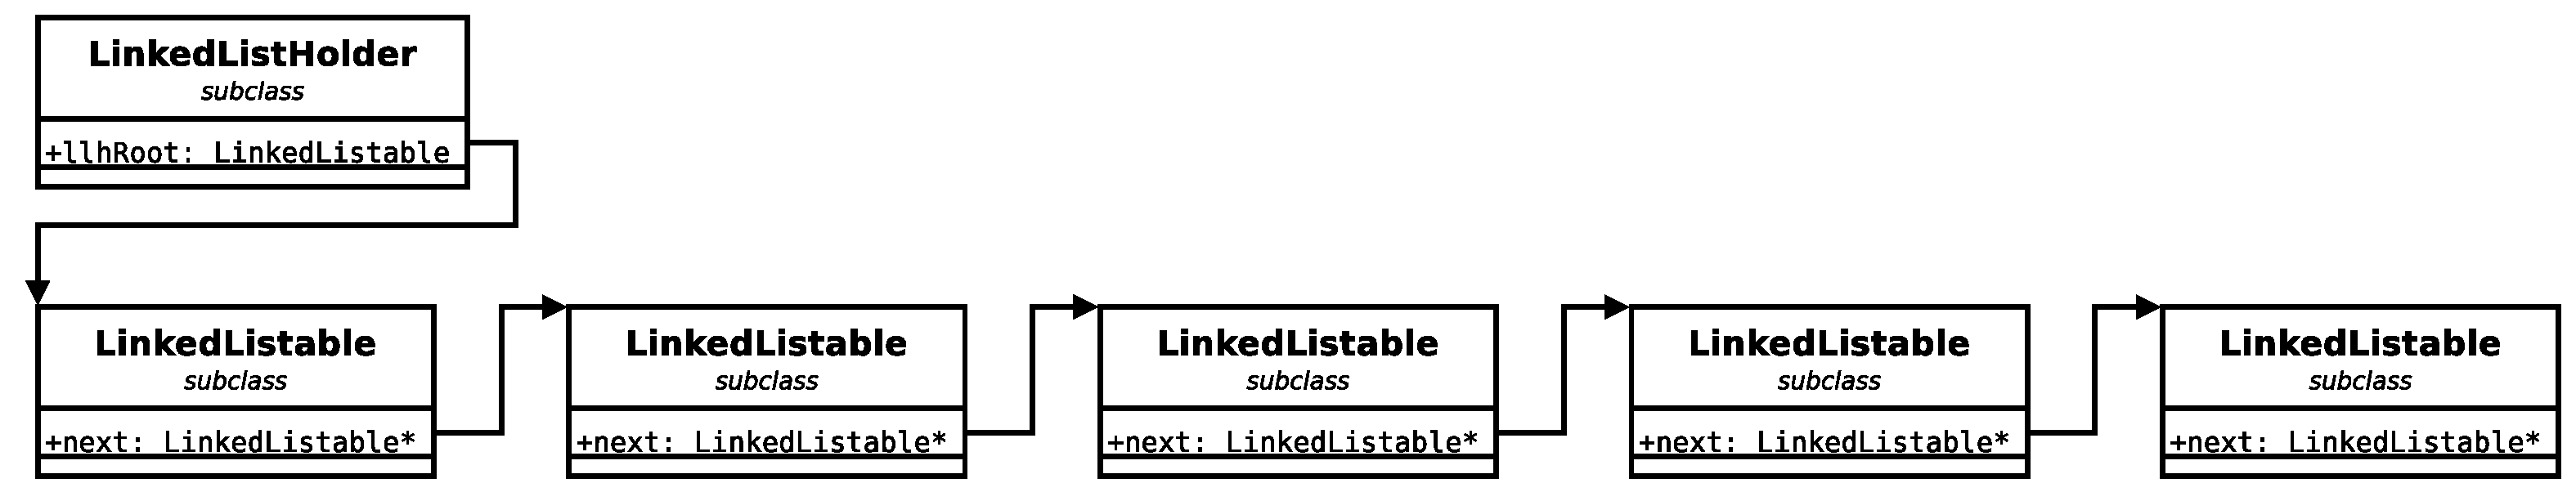
\includegraphics[width=\textwidth]{level0/linkedlist.eps}
  \caption{BaseLib Level0 linked list schema}
  \label{f:level0:linkedlist}
 \end{center}
\end{figure}

A \texttt{LinkedListHolder} is like a list container. Operations on Lists are permitted, the basic informations it holds is the first \texttt{LinkedListable} node of the list and the list size in integers.

\begin{lstlisting}[
extendedchars=true,%
basicstyle=\fontfamily{pcr}\fontseries{m}\selectfont\footnotesize, %
stepnumber=1,%
numberstyle=\tiny,%
keywordstyle=\footnotesize\tt ,%
language=C++]
protected:
   LinkedListable  llhRoot;
   uint32          llhSize;
\end{lstlisting}

\texttt{CleanUp} will deallocate all the contents and then sets the pointer to \texttt{llhRoot->next} to \texttt{NULL} and \texttt{llhSize} to zero, the \texttt{Reset} method does the same but doesn't deallocate content. 

The \texttt{List} method return the first element on the list (\texttt{llhRoot->next}) while \texttt{ListSize} return the size of the linked list (\texttt{llhSize}).

\begin{lstlisting}[
extendedchars=true,%
basicstyle=\fontfamily{pcr}\fontseries{m}\selectfont\footnotesize, %
stepnumber=1,%
numberstyle=\tiny,%
keywordstyle=\footnotesize\tt ,%
language=C++]
public:
   void CleanUp();
   void Reset();

   LinkedListable *List() const;
   uint32 ListSize()const;
\end{lstlisting}

The method \texttt{FastListInsertSingle} insert a single \texttt{LinkedListable} element \texttt{p} as the unique element of the queue.
Overloaded method \texttt{ListInsert} let the user insert a \texttt{LinkedListable} element as the first element or in an ordered way using sorters, rather of \texttt{ListInsertL} manipulate \texttt{LinkedListHolder} elements.\\


Method \texttt{ListAdd} add one single \texttt{LinkedListable} element at the end of the queue; \texttt{ListAddL} add a list of \texttt{LinkedListable} elements at the end of the queue. \\


\begin{lstlisting}[
extendedchars=true,%
basicstyle=\fontfamily{pcr}\fontseries{m}\selectfont\footnotesize, %
stepnumber=1,%
numberstyle=\tiny,%
keywordstyle=\footnotesize\tt ,%
language=C++]
   inline void FastListInsertSingle(LinkedListable &p);
   void ListInsert(LinkedListable *p);
   void ListInsert(LinkedListable *p,SortFilter *sorter);
   void ListInsert(LinkedListable *p,SortFilterFn *sorter);
   void ListInsert(LinkedListable *q,uint32 index);
   void ListInsertL(LinkedListHolder *p);
   void ListInsertL(LinkedListHolder *p,SortFilter *sorter);
   void ListInsertL(LinkedListHolder *p,SortFilterFn *sorter);
   void ListInsertL(LinkedListHolder *p,uint32 index);

   void ListAdd(LinkedListable *p);
   void ListAddL(LinkedListable *p);
\end{lstlisting}

\texttt{ListSearch} methods search the list comparing the element comparing with the one passed by argument or using a \texttt{SearchFilter} or a \texttt{SearchFilterFn}. Overloaded methods \texttt{ListExtract} do the same job as \texttt{ListSearch} but removing the element founded. \texttt{ListDelete} is the same as \texttt{ListExtract} but never return the object founded. Function \texttt{ListSafeDelete} is a special \texttt{ListDelete} version that is safe from reentrance from destructor of object (complex graph destruction). \\


Methods \texttt{ListBSort} simply sort the linked list using the sorter passed as an argument. \texttt{ListPeek} looks into the list an treat it as an array it will return the \texttt{index}-n element of the linked list. \texttt{ListIterate} methods associate an iterator to the linked list. \\


\begin{lstlisting}[
extendedchars=true,%
basicstyle=\fontfamily{pcr}\fontseries{m}\selectfont\footnotesize, %
stepnumber=1,%
numberstyle=\tiny,%
keywordstyle=\footnotesize\tt ,%
language=C++]
   bool ListSearch(LinkedListable *p);
   LinkedListable *ListSearch(SearchFilter *filter);
   LinkedListable *ListSearch(SearchFilterFn *filter);

   bool ListExtract(LinkedListable *p);
   LinkedListable *ListExtract(SearchFilter *filter);
   LinkedListable *ListExtract(SearchFilterFn *filter);
   LinkedListable *ListExtract(uint32 index=0);

   bool ListDelete(LinkedListable *p);
   bool ListDelete(SearchFilter *filter);
   bool ListSafeDelete(SearchFilter *filter);
   bool ListDelete(SearchFilterFn *filter);

   void ListBSort(SortFilter *sorter);
   void ListBSort(SortFilterFn *sorter);

   LinkedListable *ListPeek(uint32 index);

   void ListIterate(Iterator *it);
   void ListIterate(IteratorFn *it);
\end{lstlisting}



\subsubsection{StackHolder}
\texttt{[StackHolder.h]} \\
A stack data structure is simply developed on top of the single linked list abstraction. Inserting (push) elements on the head of the list and removing (pop) elements (one at a time) always from the head of the list. Such operations require only a single linked list (i.e. no double linked list is required). Figure \ref{f:level0:linked} show that a \texttt{StackHolder} is a subclass of a \texttt{LinkedListHolder} so is a linked list container but adds the tipical method a stack will have. \\


The typename \texttt{Stackable} is just a rename of the \texttt{LinkedListable} type, it is defined like below in file \texttt{level0/Iterators.h}.

\begin{lstlisting}[
extendedchars=true,%
basicstyle=\fontfamily{pcr}\fontseries{m}\selectfont\footnotesize, %
stepnumber=1,%
numberstyle=\tiny,%
keywordstyle=\footnotesize\tt ,%
language=C++]
typedef LinkedListable Stackable;
\end{lstlisting}

\texttt{StackFastPushSingle} method and pop's \texttt{StackFastPop} let you push and pop a single \texttt{Stackable} (\texttt{LinkedListable}) element from the stack. \texttt{StackPush} and \texttt{StackPop} are more slow to execute but let you add not a single element but also a linked list (or another stack).

\begin{lstlisting}[
extendedchars=true,%
basicstyle=\fontfamily{pcr}\fontseries{m}\selectfont\footnotesize, %
stepnumber=1,%
numberstyle=\tiny,%
keywordstyle=\footnotesize\tt ,%
language=C++]
public:
   inline void StackFastPushSingle(Stackable *p);
   inline Stackable *StackFastPop();

   void StackPush(Stackable *p);
   Stackable *StackPop();
\end{lstlisting}

Last methods are the same as the \texttt{LinkedListHolder} implementation let only the user call those methods with a more friendly ``stackable'' name.

\begin{lstlisting}[
extendedchars=true,%
basicstyle=\fontfamily{pcr}\fontseries{m}\selectfont\footnotesize, %
stepnumber=1,%
numberstyle=\tiny,%
keywordstyle=\footnotesize\tt ,%
language=C++]
   uint32 StackDepth();
   Stackable *StackPeek(uint32 index);
   Stackable *StackTop();
   Stackable *StackExtract(uint32 index);
   void StackInsert(Stackable *q,uint32 index);
\end{lstlisting}

This class is really simply and each method usually call the same method of the superclass.



\subsubsection{QueueHolder}
\texttt{[QueueHolder.h]}\\
\texttt{QueueHolder} is a class that can handle a queue of \texttt{Queueable} elements; the typename \texttt{Queueable} is just an alias of the \texttt{LinkedListable} type, it is defined like below in file \texttt{level0/Iterators.h}.

\begin{lstlisting}[
extendedchars=true,%
basicstyle=\fontfamily{pcr}\fontseries{m}\selectfont\footnotesize, %
stepnumber=1,%
numberstyle=\tiny,%
keywordstyle=\footnotesize\tt ,%
language=C++]
typedef LinkedListable Queueable;
\end{lstlisting}

A queue data structure is simply depicted in Figure \ref{f:level0:queue}.

\begin{figure}[h!]
 \begin{center}
  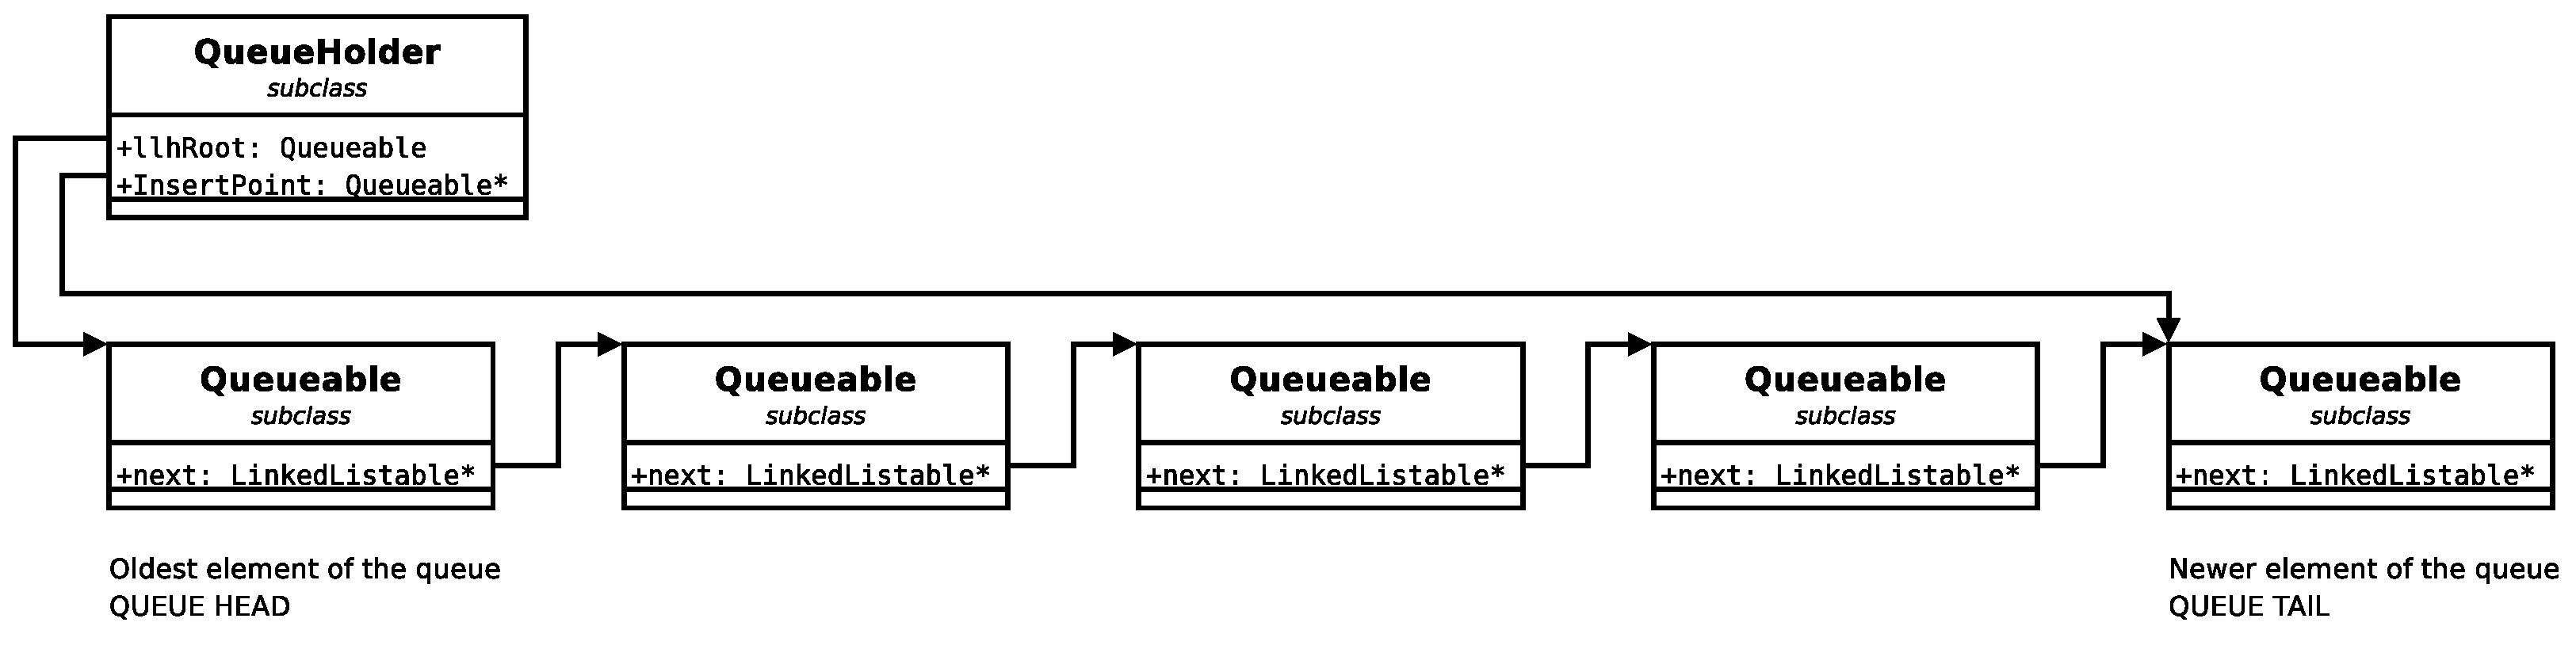
\includegraphics[width=\textwidth]{level0/queue.eps}
  \caption{BaseLib Level0 queue schema}
  \label{f:level0:queue}
 \end{center}
\end{figure}

The \texttt{QueueHolder} class add the protected attribute \texttt{insertionPoint} to the \texttt{StackHolder} class; in this way mantaining only a single linked list with only the \textit{next} pointer it has a full control of the queue knowing the head and tail elements, navigation of the queue remain possible only in one direction, no bidirectional navigation could be possible. In this way removing elements at the tail is very time consuming; the design allows removing elements only from the head of the queue.

\begin{lstlisting}[
extendedchars=true,%
basicstyle=\fontfamily{pcr}\fontseries{m}\selectfont\footnotesize, %
stepnumber=1,%
numberstyle=\tiny,%
keywordstyle=\footnotesize\tt ,%
language=C++]
protected:
   Queueable *insertionPoint;
\end{lstlisting}

The \textit{oldest} element is the element at the head of the queue and is also the oldest added to it. The insertion of a new element will be made at the tail of the queue.\\


The method \texttt{Oldest} return the oldest inserted element in the queue, returning doesn't mean extracting infact the element still reamin in the queue. Note that it is possible to return only one element at a time. The extraction activity is done by the \texttt{QueueExtract} method that return and remove the oldest element on the queue. Last \texttt{QueueExtract} search from the oldest \texttt{Queueable} item the element passed by argument and remove it.\\


The \texttt{QueueAdd} method add on the queue head the passed by \texttt{Queueable} elements, it is possible to add also a list of \texttt{Queueable}s. \texttt{FastQueueInsertSingle} does the same but add to the queue only one element at a time.
\texttt{QueueInsert} insert the passed by argument \texttt{Queueable} element/s resetting all the content of the queue to it/them; use it with care because can remove all elements in the queue.

\begin{lstlisting}[
extendedchars=true,%
basicstyle=\fontfamily{pcr}\fontseries{m}\selectfont\footnotesize, %
stepnumber=1,%
numberstyle=\tiny,%
keywordstyle=\footnotesize\tt ,%
language=C++]
public:
   Queueable *Oldest();
   Queueable *QueueExtract();
   bool QueueExtract(Queueable *p);

   void QueueAdd(Queueable *p); 
   inline void FastQueueInsertSingle(LinkedListable &p);
   void QueueInsert(Queueable *p);
\end{lstlisting}

Methods \texttt{QueuePeek} and \texttt{QueuePeekLast} do not remove the required element from the queue; the first one do not do any check on queue boundary before performing the peek action.
\texttt{Reset} method simply call the superclass one removing one by one elements from the list. Elements could be not more refereneced and so can be lost wasting memory.

\begin{lstlisting}[
extendedchars=true,%
basicstyle=\fontfamily{pcr}\fontseries{m}\selectfont\footnotesize, %
stepnumber=1,%
numberstyle=\tiny,%
keywordstyle=\footnotesize\tt ,%
language=C++]
   Queueable *QueuePeek(uint32 index);
   Queueable *QueuePeekLast();

   void Reset();
   uint32 QueueSize();
\end{lstlisting}



\subsubsection{Iterator, IteratorT, IteratorFn}
\texttt{[Iterator.h]}\\
The \texttt{Iterator} class define only one pure virtual function so it is a C++ interface. The function is defined as:

\begin{lstlisting}[
extendedchars=true,%
basicstyle=\fontfamily{pcr}\fontseries{m}\selectfont\footnotesize, %
stepnumber=1,%
numberstyle=\tiny,%
keywordstyle=\footnotesize\tt ,%
language=C++]
public:
   virtual void Do (LinkedListable* data)=0;
\end{lstlisting}

The \texttt{Do} function perform the iteration passing a \texttt{LinkedListable} element as an argument. 
\texttt{IteratorT} is a more specialised version of the \texttt{Iterator} letting the developer not to specify a \texttt{LinkedListable} element or a subclass of it in the \texttt{Do} method. \texttt{IteratorT} is also an interface.

\texttt{IteratorFn} is simply a typedef defined as follow:

\begin{lstlisting}[
extendedchars=true,%
basicstyle=\fontfamily{pcr}\fontseries{m}\selectfont\footnotesize, %
stepnumber=1,%
numberstyle=\tiny,%
keywordstyle=\footnotesize\tt ,%
language=C++]
typedef void (IteratorFn )(LinkedListable* data);
\end{lstlisting}



\subsubsection{SearchFilter, SearchFilterT, SearchFilterFn}
\texttt{[Iterator.h]}\\
The \texttt{SearchFilter} class define only one pure virtual function so it is a C++ interface. The function is defined as:

\begin{lstlisting}[
extendedchars=true,%
basicstyle=\fontfamily{pcr}\fontseries{m}\selectfont\footnotesize, %
stepnumber=1,%
numberstyle=\tiny,%
keywordstyle=\footnotesize\tt ,%
language=C++]
public:
   virtual bool Test (LinkedListable* data)=0;
\end{lstlisting}

The \texttt{Test} function perform the search on a set of data passing a \texttt{LinkedListable} element as an argument. A new class that implement the searching activity must be defined.
\texttt{SearchFilterT} is a more specialised version of the \texttt{SearchFilter} letting the developer not to specify a \texttt{LinkedListable} element or a subclass of it in the \texttt{Test} method. \texttt{SearchFilterT} is also an interface.

\texttt{SearchFilterFn} is simply a typedef defined as follow:

\begin{lstlisting}[
extendedchars=true,%
basicstyle=\fontfamily{pcr}\fontseries{m}\selectfont\footnotesize, %
stepnumber=1,%
numberstyle=\tiny,%
keywordstyle=\footnotesize\tt ,%
language=C++]
typedef bool (SearchFilterFn )(LinkedListable* data);
\end{lstlisting}



\subsubsection{SortFilter, SortFilterFn}
\texttt{[Iterator.h]}\\
The \texttt{Iterator} class define only one pure virtual function so it is a C++ interface. The function is defined as:

\begin{lstlisting}[
extendedchars=true,%
basicstyle=\fontfamily{pcr}\fontseries{m}\selectfont\footnotesize, %
stepnumber=1,%
numberstyle=\tiny,%
keywordstyle=\footnotesize\tt ,%
language=C++]
public:
   virtual void Do (LinkedListable* data)=0;
\end{lstlisting}

The \texttt{Do} function perform the iteration passing a \texttt{LinkedListable} element as an argument. 
\texttt{IteratorT} is a more specialised version of the \texttt{Iterator} letting the developer not to specify a \texttt{LinkedListable} element or a subclass of it in the \texttt{Do} method. \texttt{IteratorT} is also an interface.

\texttt{IteratorFn} is simply a typedef defined as follow:

\begin{lstlisting}[
extendedchars=true,%
basicstyle=\fontfamily{pcr}\fontseries{m}\selectfont\footnotesize, %
stepnumber=1,%
numberstyle=\tiny,%
keywordstyle=\footnotesize\tt ,%
language=C++]
typedef void (IteratorFn )(LinkedListable* data);
\end{lstlisting}

TODO \\
TODO \\
TODO \\
thanks Ric \\
aggiugere qualche esempio di utilizzo (ps prendi il libro di dati e algoritmi)


\subsubsection{DirectoryEntry}
\texttt{[Directory.h]}
Such \texttt{DirectoryEntry} class represent a file or a subdirectory. Usually a directory structure is a tree data structure but such class is implemented using a single linked list; this abstraction doesn't represent a tree of files or directories but simply the directory content, letting navigate in an OS directory.\\


There are three private attributes: the file or subdirectory name, some statistics about the file and a pointer to a \texttt{Directory} conteiner that is a \texttt{LinkedListHolder}.

\begin{lstlisting}[
extendedchars=true,%
basicstyle=\fontfamily{pcr}\fontseries{m}\selectfont\footnotesize, %
stepnumber=1,%
numberstyle=\tiny,%
keywordstyle=\footnotesize\tt ,%
language=C++]
private:
   const char* fname;
   struct stat fileStatistics;
   Directory* holder;
\end{lstlisting}

Such attributes let the \texttt{Directory} and \texttt{DirectoryEntry} classes change the \texttt{LinkedListHolder} and \texttt{LinkedListable} structure to showed in Figure \ref{f:level0:directory}.

\begin{figure}[h!]
 \begin{center}
  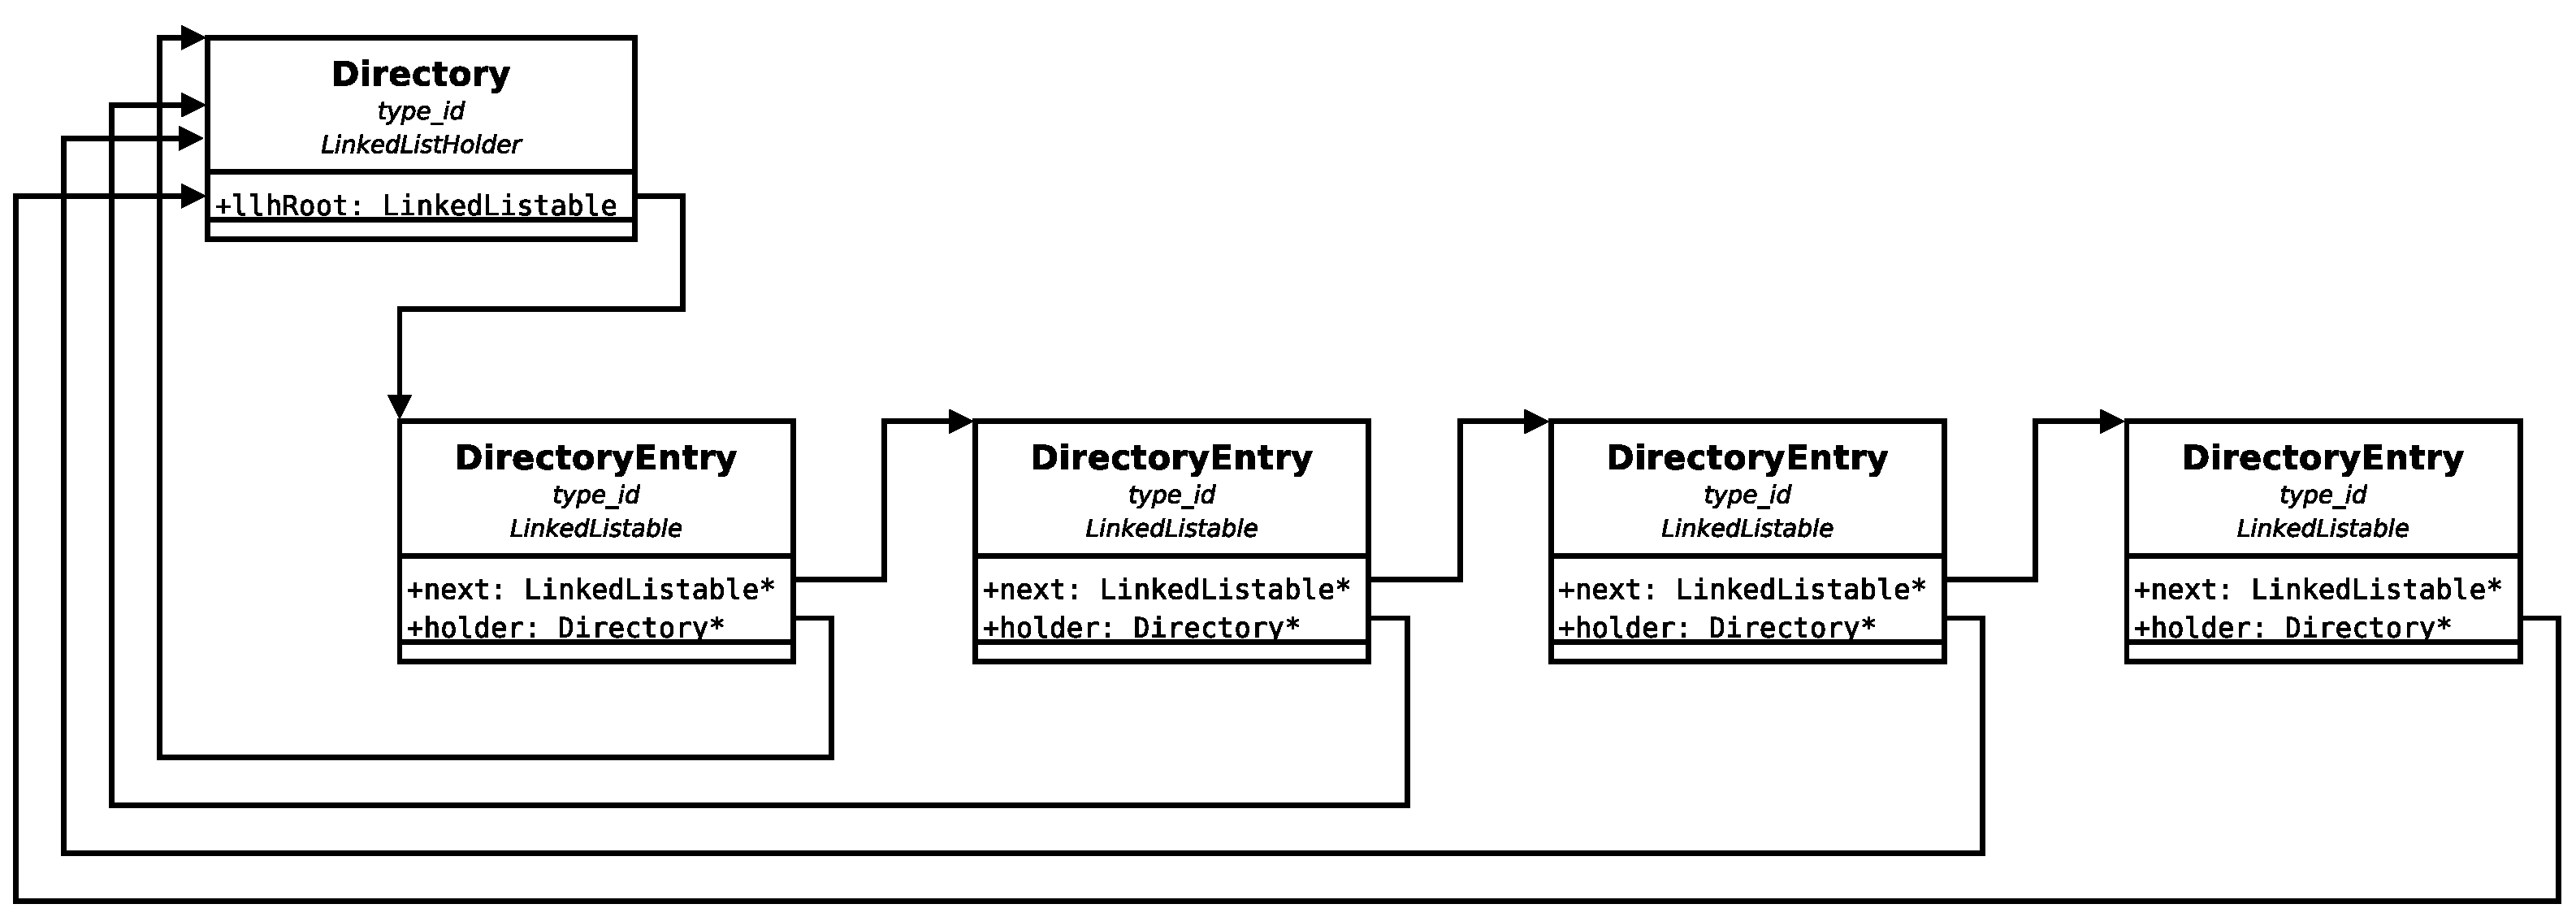
\includegraphics[width=\textwidth]{level0/directory.eps}
  \caption{BaseLib Level0 Directory scheme}
  \label{f:level0:directory}
 \end{center}
\end{figure}

A creation time the developer must supply the \texttt{Directory} container and the name of the file or subdirectory.
The \texttt{Name} method return the name of the file or subdirectory and the methods \texttt{IsDirectory} and \texttt{IsFile} let you check if the instance represent a directory or a file.


\texttt{ReadOnly} let you query if the file has the \textit{read only} attribute, \texttt{Size} method return the size of the file. The method \texttt{Time} return the last write time and \texttt{LastAccessTime} get the last access time.

\begin{lstlisting}[
extendedchars=true,%
basicstyle=\fontfamily{pcr}\fontseries{m}\selectfont\footnotesize, %
stepnumber=1,%
numberstyle=\tiny,%
keywordstyle=\footnotesize\tt ,%
language=C++]
public:
   DirectoryEntry(Directory *holder, const char *fname = NULL);
   ~DirectoryEntry();

   const char* Name();
   bool IsDirectory();
   bool IsFile();

   bool ReadOnly();
   int64 Size();

   time_t Time();
   time_t LastAccessTime();
\end{lstlisting}



\subsubsection{Directory}
\texttt{[Directory.h]}
The \texttt{Directory} class contains information about a directory and all its content. It basically hold a single linked list of \texttt{DirectoryEntry} that can be file and/or subdirectory names. \\


A \texttt{Directory} is identified by a path in the FileSystem hierical on each common OS nowadays. So the first attribute of the class is the path of the directory to be listed \texttt{baseAddress}; the second attribute is the size of the entire directory \texttt{size}.

\begin{lstlisting}[
extendedchars=true,%
basicstyle=\fontfamily{pcr}\fontseries{m}\selectfont\footnotesize, %
stepnumber=1,%
numberstyle=\tiny,%
keywordstyle=\footnotesize\tt ,%
language=C++]
private:
   char* baseAddress;
   uint64 size;
\end{lstlisting}

Such class has only few methods; the constructor does the major stuff. The constructor require the path of the directory a file mask and a sorter, in this way it is possible to have a list of only the file of a certain format.
\texttt{TotalFileSize} simply return the \texttt{size} attribute.\\


The two static methods are currently coded only for Windows platforms and let the user create a directory and test for directory existance.

\begin{lstlisting}[
extendedchars=true,%
basicstyle=\fontfamily{pcr}\fontseries{m}\selectfont\footnotesize, %
stepnumber=1,%
numberstyle=\tiny,%
keywordstyle=\footnotesize\tt ,%
language=C++]
public:
   Directory(const char* address,const char* fileMask="*",SortFilterFn* sorter=NULL);
   uint64 TotalFileSize();

   static bool Create(const char* address);
   static bool DirectoryExists(const char* address);
\end{lstlisting}



\subsection{Static Lists}
\begin{figure}[h!]
 \begin{center}
  \includegraphics[width=0.55\textwidth]{level0/level0-static.eps}
  \caption{BaseLib Level0 Static Lists classes}
  \label{f:level0:static}
 \end{center}
\end{figure}

Static Lists are basically \textit{arrays} or \textit{vectors}. Such structure contains 32bit pointers or any other structure. This list of pointers can grow and shrink and the reallocation is done by the class itself using library routines like \texttt{malloc} and \texttt{realloc}. It obvioulsy allows inserting and removing of elements. It also offers the possibility to control the data access via a semaphore.


Class diagram is depicted in Figure \ref{f:level0:static}, classe in this group are:

\begin{itemize}
 \item StaticListHolder
 \item StaticStackHolder
 \item StaticQueueHolder

 \item StaticListTemplate
\end{itemize}

Static list classes are written with the aim of mantaining the same methods signatures of the Linked List interface.



\subsubsection{StaticListHolder}
\texttt{[StaticListHolder.h]}\\
The main data structure that hold all the data is an array; this array is dynamically allocated at run-time and is pointed from the \texttt{elements} attribute. Such pointer point to 32bit integers, this integers are usually 32bit pointers, but can be also a structures of the same size; the constructor let you create an array with elements of a size multiple of 32bit. So the \textit{StaticList} can hold 32bit ptr or 64bit ptr or any other structure.
The protected attribute \texttt{elementSize32bit} give you the size of one item on the \textit{StaticList}; the \texttt{numberOfElements} give the number of items in the \textit{StaticList}, the \texttt{FastPollingMutexSem} give a way to allow multiple threads protected access to the data and the \texttt{msecTimeout} is the timeout to wait on the semaphore for catching the resource.

\begin{lstlisting}[
extendedchars=true,%
basicstyle=\fontfamily{pcr}\fontseries{m}\selectfont\footnotesize, %
stepnumber=1,%
numberstyle=\tiny,%
keywordstyle=\footnotesize\tt ,%
language=C++]
protected:
   int32* elements;
   int elementSize32bit;
   int numberOfElements;

   FastPollingMutexSem mux;
   TimeoutType msecTimeout;
\end{lstlisting} 

The following protected methods are self explained and are used to grow and shrink the ata structure, copy and move datas and finding and indexing an element in the \texttt{StaticListHolder}. Comments are left.

\begin{lstlisting}[
extendedchars=true,%
basicstyle=\fontfamily{pcr}\fontseries{m}\selectfont\footnotesize, %
stepnumber=1,%
numberstyle=\tiny,%
keywordstyle=\footnotesize\tt ,%
language=C++]
   /** increases the list size by 1.
       Manages the reallocation of memory when necessary */
   bool IncreaseListSize();
   /** decreases the list size by 1.
       Reallocation of memory is not performed */
   bool DecreaseListSize();

   /** copies data from a buffer to the position */
   inline void Copy(int32 *destination,const int32 *source);
   /** compares data between source and destination. True means equal */
   inline bool Compare(const int32 *destination,const int32 *source);
   /** finds data in list. -1 means not found */
   inline int Find(const int32 *data);

   /** retrieves address of data element */
   inline int32* GetPointer(int position);
   /** moves all the pointers from position to the right.
       Assumes that the last position is empty */
   inline void RightShiftListFrom(int position);
   /** removes the element in position and shifts all the elements 
       at the right of it to the left */
   inline void LeftShiftListTo(int position);
\end{lstlisting}

Public methods have the same names as \texttt{LinkedListHolder}'s methods, arguments differ. The size of the elements, in 4byte units, is defined by the constructor and is no more modificable.\\


To control multiple access it is possible to set a timeout on the waiting operation, the timeout can be set with \texttt{SetAccessTimeout}. To retrieve the number of elements in the \texttt{StaticList} use \texttt{ListSize}.\\


\texttt{ListAdd} add one element at any specified position; as a shortcut if the element must be added at the top of the list you can pass 0 as at position argument and -1 for the end of the list; \texttt{ListInsert} simply add the element at the top of the array.

The method \texttt{ListFind} finds at what index the specified data is located, it returns -1 if doesn't found any matching object.

\texttt{ListExtract} removes an element from any position, if \texttt{position} is 0 it removes from the top, if -1 removes from the end; \texttt{element} is a pointer to a buffer of data that the will be filled by the method. \texttt{ListPeek} reads an item from the data structure without affecting the list; \texttt{element} argument is a pointer to a buffer of data that will be copied from the list. The method \texttt{ListDelete} removes an element from the list using a copy of the \texttt{element} as a search key. The last \texttt{ListDelete} removes at the specified indexed position.

\begin{lstlisting}[
extendedchars=true,%
basicstyle=\fontfamily{pcr}\fontseries{m}\selectfont\footnotesize, %
stepnumber=1,%
numberstyle=\tiny,%
keywordstyle=\footnotesize\tt ,%
language=C++]
public:
   StaticListHolder(int elementSize32bit = 1);
   virtual ~StaticListHolder();

   void SetAccessTimeout(TimeoutType  msecTimeout = TTInfiniteWait);
   uint32 ListSize()const;

   bool ListAdd(const int32 *element,int position = SLH_EndOfList);
   inline void ListInsert(int32 *element);

   int ListFind(const int32 *element);

   bool ListExtract(int32 *element=NULL,int position = SLH_EndOfList);
   bool ListPeek(int32 *element=NULL,int position = SLH_EndOfList);
   bool ListDelete(const int32 *element);
   inline bool ListDelete(int position);
\end{lstlisting}



\subsubsection{StaticStackHolder}
\texttt{[StaticStackHolder.h]}\\
This class is try to mimic the same API of StackHolder but relaying on arrays.
The constructor creates a stack with the given element size (note that the size is in 32 bit multiples), the size of the stack my vary during run time.
\texttt{StackPush} insert on top a single element. When the space is finished the bottom is discarded; \texttt{StackPop} get an element from top of the array and remove it from the stack; for not removing the element from the stack use \texttt{StackTop}.
Method \texttt{StackPeek} looks into the stack for an element with the given index \texttt{position}.
\texttt{StackDepth} return the number of elements in the stack.

\begin{lstlisting}[
extendedchars=true,%
basicstyle=\fontfamily{pcr}\fontseries{m}\selectfont\footnotesize, %
stepnumber=1,%
numberstyle=\tiny,%
keywordstyle=\footnotesize\tt ,%
language=C++]
public:
   StaticStackHolder(int elementSize32bit=1);

   inline void StackPush(const int32* element);
   inline bool StackPop(int32* element);
   inline bool StackTop(int32* element);
   inline bool StackPeek(int32* element,int position);

   inline uint32 StackDepth();
\end{lstlisting}



\subsubsection{StaticQueueHolder}
\texttt{[StaticQueueHolder.h]}\\
This class is still try to mimic the same API of QueueHolder but relaying on arrays.
Like the \texttt{StaticStackHolder} and the superclass \texttt{StatiListHolder} this class require the size of the elements in 32bit units in the constructor. \texttt{QueueSize} return the number of elements in the queue.
\texttt{QueueAdd} insert an element on the queue, \texttt{Last} return the last inserted element in the queue, \texttt{QueueExtract} removes the oldest element from the queue; \texttt{QueuePeek} looks into the queue, index 0 is the most recent added; \texttt{QueuePeekLast} looks into the queue to the last element inserted.

\begin{lstlisting}[
extendedchars=true,%
basicstyle=\fontfamily{pcr}\fontseries{m}\selectfont\footnotesize, %
stepnumber=1,%
numberstyle=\tiny,%
keywordstyle=\footnotesize\tt ,%
language=C++]
public:
   StaticQueueHolder(int elementSize32bit = 1);

   inline void QueueAdd(const int32* element);
   inline bool Last(int32* element);
   inline bool QueueExtract(int32* element);
   inline bool QueuePeek(int32* element,uint32 index);
   inline bool QueuePeekLast(int32* element);

   inline uint32 QueueSize();
\end{lstlisting}



\subsubsection{StaticListTemplate}
\texttt{[StaticListTemplate.h]}\\
This class is a template to customise a \texttt{StaticListHolder} for a specific struct or class. Such class is a subclass of the \texttt{StaticListHolder}. This class is never used in BaseLib. This class lets specializing the superclass for a particular type of object. Using such specialized class you have an array of object of the same size of the object templatized for. The interface, really similar to the \texttt{StaticListHolder} one follows.

\begin{lstlisting}[
extendedchars=true,%
basicstyle=\fontfamily{pcr}\fontseries{m}\selectfont\footnotesize, %
stepnumber=1,%
numberstyle=\tiny,%
keywordstyle=\footnotesize\tt ,%
language=C++]
public:
   StaticListTemplate(TimeoutType  msecTimeout = TTInfiniteWait);

   inline bool ListAdd(const T &element,int position=SLH_EndOfList)
   inline void ListInsert(const T &element);

   inline bool ListExtract(T &element,int position=SLH_EndOfList)
   inline bool ListPeek(T &element,int position = SLH_EndOfList)
   inline bool ListDelete(const T &element);
   inline bool ListDelete(int position);

   inline int ListFind(const T &element);

   uint32 ListSize()const;
\end{lstlisting}



\subsection{Design Notes}

There is no need to typedef \texttt{LinkedListable} in \texttt{Stackable} and \texttt{Queueable} but is not an error, if there is no need to extend it with further information why aliasing it? A good choice could be to extend \texttt{LinkedListable} in \texttt{Queueable} creating a double linked list that could be a real advantage to boost the performance of walking a list.\\

 (why not call them symmetrically? Like \texttt{StackFastPush} and \texttt{StackFastPop}) \\
(those function can have a more significant name like \texttt{QueueOldest} and \texttt{QueueExtract}) \\
The \texttt{QueueAdd} method add on the queue head the passed by \texttt{Queueable} elements, it is possible to add also a list of \texttt{Queueable}s. \texttt{FastQueueInsertSingle} does the same but add to the queue only one element at a time. This is another misusage of names in this section: better names can be \texttt{QueueAdd} and \texttt{QueueAddFast}. \\


Some methods, like \texttt{queueInsert} are to be used with care. \texttt{queueInsert} add elements to the queue deleting all other elements in the queue without any check or call to deletion wasting all references.\\


Sometimes there are no boundaries checks in the \textit{linked} implementation but also in the \textit{static} implementation.\\


Probably there is a lack of a Template, look at \textit{level0/Iterator.h} there are those declariotions: \texttt{Iterator}, \texttt{IteratorFn}, \texttt{IteratorT}; \texttt{SearchFilter}, \texttt{SearchFilterFn}, \texttt{SearchFilterT}; \texttt{SortFilter}, \texttt{SortFiletrFn} and \texttt{SortFilterT} is not defined.\\


The \texttt{Directory} pair of classes must be ported also on other OSes. The \texttt{Driectory} structure can be developed on a tree data structure instead on a single linked list. So there is the need to add the tree data structure to this data structure section. \\


The \texttt{StaticQueue} structure will be better developed on a circular buffer instead on a \texttt{StaticListHolder}. Will be more processor efficient.\\



\section{IPC}
This group of classes add the semaphore abstraction and the spinlock mechanism to the BaseLib library. Figure \ref{f:level0:ipc} illustrate the classes structure, semaphores and spinlocks, of a great interest is the \textit{SemNameDataBase}.

\begin{figure}[h!]
 \begin{center}
  \includegraphics[width=\textwidth]{level0/level0-IPC.eps}
  \caption{BaseLib Level0 IPC classes}
  \label{f:level0:ipc}
 \end{center}
\end{figure}



\subsection{Semaphores}
A semaphore is one of the simplest Inter Processes Communication mechanisms. BaseLib introduce different types of semaphores. One of the most important functionality it adds is the \textit{SemNameDataBase} that is a list of all BaseLib's semaphores created run-time. Such stuff lets the developer exploits named semaphores on each Operating System.

\begin{figure}[h!]
 \begin{center}
  \includegraphics[width=\textwidth]{level0/level0-IPC-Sem.eps}
  \caption{BaseLib Level0 semaphore classes}
  \label{f:level0:ipc-sem}
 \end{center}
\end{figure}

Figure \ref{f:level0:ipc-sem} depict semaphore classes in this section (other classes previously anlized are also present: \texttt{LinkedListable}, \texttt{LinkedListHolder} and \texttt{SearchFilter}):
\begin{itemize}
 \item SemInfoBits
 \item SemNameDB
 \item SemNameFinder, SemPurger

 \item SemCore
 \item EventSem
 \item MutexSem
 \item MuxLock
\end{itemize}

We are going first to explore the \textit{SemNameDataBase} architecture. The OS2 naming convention is used in this group of classes, in OS2 there are \texttt{EventSem} and \texttt{MutexSem}. Follow a table that summarizes some differences between ipc's API in OS/2, POSIX.1b (UNIX, System V) and POSIX.1c (pthread). The mapping between OS/2 and POSIX.1b is not straightforward.

\begin{table}[!h]
 \begin{center}
  \begin{tabular}{|l|l|l|}
   \hline
    OS/2 & POSIX.1c & POSIX.1b \\
   \hline
    \texttt{DosCreateMutexSem} & \texttt{pthread\_mutex\_init} & \texttt{sem\_init} \\
   \hline
    \texttt{DosRequestMutexSem} & \texttt{pthread\_mutex\_lock} / & \texttt{sem\_wait} / \\
     & \texttt{pthread\_mutex\_trylock} & \texttt{sem\_trywait} \\
   \hline
    \texttt{DosReleaseMutexSem} & \texttt{pthread\_mutex\_unlock} & \texttt{sem\_post} \\
   \hline
    \texttt{DosCloseMutexSem} & \texttt{pthread\_mutex\_destroy} & \texttt{sem\_destroy} \\
   \hline
    \texttt{DosCreateEventSem} & \texttt{pthread\_cond\_init} & \texttt{sem\_init} \\
   \hline
    \texttt{DosWaitEventSem} & \texttt{pthread\_cond\_signal\_wait} / & \texttt{sem\_wait} / \\
     & \texttt{pthread\_cond\_timedwait} & \texttt{sem\_trywait} \\
   \hline
    \texttt{DosPostEventSem} & \texttt{pthread\_cond\_signal} / & \texttt{sem\_post} \\
     & \texttt{pthread\_cond\_broadcast} & \\
   \hline
    \texttt{DosCloseEventSem} & \texttt{pthread\_cond\_destroy} & \texttt{sem\_destroy} \\
   \hline
   \end{tabular}
   \end{center}
  \caption{Basic IPC in OS2, POSIX.1b (UNIX, System V) and POSIX.1c (pthread)}
 \label{t:ipc_api}
\end{table}

Table \ref{t:ipc_api} must clarify the mapping between \textit{EventSem} in OS/2 and \textit{Conditional Variables} in POSIX.1c and between \textit{MutexSem} and \textit{mutex} in POSIX.1c.



\subsubsection{SemInfoBits}
\texttt{[SemCore.cpp]}\\
The class \texttt{SemInfoBits} is a \texttt{LinkedListable} list item of the \texttt{SemNameDataBase} (that is a \texttt{LinkedListHolder}). There is a \texttt{SemInfoBits} list item for each semaphore istantiated in the library, for each semaphore in the DataBase we save a \texttt{name}, an \texttt{id}, some \texttt{data} and a usage count (\texttt{useCount}).

\begin{lstlisting}[
extendedchars=true,%
basicstyle=\fontfamily{pcr}\fontseries{m}\selectfont\footnotesize, %
stepnumber=1,%
numberstyle=\tiny,%
keywordstyle=\footnotesize\tt ,%
language=C++]
private:
   char* name;
   SEM_ID id;
   void* data;
public:
   int32 useCount;
\end{lstlisting}

All methods are public and except the constructor there are only get methods that let you retrieve attributes value.

\begin{lstlisting}[
extendedchars=true,%
basicstyle=\fontfamily{pcr}\fontseries{m}\selectfont\footnotesize, %
stepnumber=1,%
numberstyle=\tiny,%
keywordstyle=\footnotesize\tt ,%
language=C++]
   SemInfoBit(SEM_ID id,char* name,void* data);
   ~SemInfoBit();

   char* Name();
   SEM_ID Id();
   void* Data();
\end{lstlisting}



\subsubsection{SemNameDB}
\texttt{[SemCore.cpp]}\\
The \texttt{SemNameDataBase} is the only instance of the \texttt{SemNameDB}; it holds the run-time database of all semaphores alive in the system.
Such class extends \texttt{LinkedListHolder} adding the three methods below that let the user adding and deleting a semaphore in the list and getting its identifier as a \texttt{SEM\_ID} data type.

\begin{lstlisting}[
extendedchars=true,%
basicstyle=\fontfamily{pcr}\fontseries{m}\selectfont\footnotesize, %
stepnumber=1,%
numberstyle=\tiny,%
keywordstyle=\footnotesize\tt ,%
language=C++]
public:
   void Add(SEM_ID id,char* name,void* data=NULL);
   bool Delete(SEM_ID id);

   SEM_ID UseExisting(char *name,void *&data);
\end{lstlisting}

Data type \texttt{SEM\_ID} is a pointer or an handle, it depends on the Operating System in use.



\subsubsection{SemNameFinder, SemPurger}
\texttt{[SemCore.cpp]}\\
Those two classes represent the last part of the \textit{SemNameDataBase} implementation; togheter they let the user searching the database linked list, those classes are subclass of the \texttt{SearchFilter} class.\\


A \texttt{SemNameFinder} class must be created each time we want to search a semaphore by name and obviously we know the name. After creating the class wit is possible to use the \texttt{Test} method passing a pointer to a \texttt{LinkedListable} element and know if there is a semaphore with that name in the sublist passed by argument. The class interface follow. The attirbute \texttt{checkCount} is not used right now. Such class must be used to wuery about the existence of a particular semaphore instance.

\begin{lstlisting}[
extendedchars=true,%
basicstyle=\fontfamily{pcr}\fontseries{m}\selectfont\footnotesize, %
stepnumber=1,%
numberstyle=\tiny,%
keywordstyle=\footnotesize\tt ,%
language=C++]
class SemNameFinder : public SearchFilter{
   char *name;
   bool checkCount;
public:
   SemNameFinder(char* name,bool checkCount=False);
   virtual ~SemNameFinder();

   bool Test(LinkedListable* data);
};
\end{lstlisting}

A \texttt{SemPurger} class behave in the same way as a \texttt{SemNameFinder} but search the \textit{SemNameDataBase} by \texttt{SEM\_ID} not by name. Just to not be symmetrically they have a different API (difficult to remember). \texttt{Found} method return the saved result of the searching activity, the class has no way to know if the search activity was just performed or not and so doesn't know about the freshness of the \texttt{found} value.

\begin{lstlisting}[
extendedchars=true,%
basicstyle=\fontfamily{pcr}\fontseries{m}\selectfont\footnotesize, %
stepnumber=1,%
numberstyle=\tiny,%
keywordstyle=\footnotesize\tt ,%
language=C++]
class SemPurger : public SearchFilter{
   SEM_ID id;
   bool found;
public:
   SemPurger(SEM_ID id);

   bool Test(LinkedListable* data);
   bool Found();
};
\end{lstlisting}



\subsubsection{SemCore}
\texttt{[SemCore.h, SemCore.cpp]}\\
The \texttt{SemCore} class isn't a semaphore or a semaphore interface instead it is an abstract class that provide OS handle registration; this class doesn't provide registration and deletion with the \textit{SemNameDataBase} that is done by the subclasses \texttt{MutexSem} and \texttt{EventSem} (see Figure \ref{f:level0:ipc-sem}), the only thing it does is managing OS handle. \\


The \texttt{Init} method set the semaphore handle to 0 or to the passed by handle; constructors call the relative \texttt{Init} function.

\begin{lstlisting}[
extendedchars=true,%
basicstyle=\fontfamily{pcr}\fontseries{m}\selectfont\footnotesize, %
stepnumber=1,%
numberstyle=\tiny,%
keywordstyle=\footnotesize\tt ,%
language=C++]
protected:
   HANDLE semH;
public:
   void Init();
   void Init(HANDLE s);

   SemCore();
   SemCore(HANDLE s);

   void operator=(SemCore& s);
   inline HANDLE Handle();
\end{lstlisting}



\subsubsection{EventSem}
\texttt{[EventSem.h]}\\
Such class define and implement an event shemaphore. Such class deal directly with the OS. Is really thightly bounded. The constructor simply set if passed by the OS semaphore handle, in this case is the user that create a semaphore. The class itself has method to create a sempahore with the OS or to find and reuse other existing registered semaphores. Is some OS the class use an helper class called \texttt{PrivateEventSemStruct}.

\begin{lstlisting}[
extendedchars=true,%
basicstyle=\fontfamily{pcr}\fontseries{m}\selectfont\footnotesize, %
stepnumber=1,%
numberstyle=\tiny,%
keywordstyle=\footnotesize\tt ,%
language=C++]
public:
   EventSem();
   EventSem(HANDLE h);
   ~EventSem();
\end{lstlisting}

To open and create a new semaphore there are several methods; \texttt{Create} create a general semaphore without a name; \texttt{CreateShared} create a named semaphore and register it in the \textit{SemNameDataBase}; \texttt{OpenExisting} query the \textit{SemNameDataBase} for the required semaphore and take a reference to it. \\


The \texttt{Close} method closes the semaphore possibly deleting it from the system if the usage count is zero; the method ask also to the \textit{SemNameDataBase} to delete it. Some more checks on the usage count must be done.

\begin{lstlisting}[
extendedchars=true,%
basicstyle=\fontfamily{pcr}\fontseries{m}\selectfont\footnotesize, %
stepnumber=1,%
numberstyle=\tiny,%
keywordstyle=\footnotesize\tt ,%
language=C++]
   bool Create();
   bool CreateShared(const char* name);
   bool OpenExisting(const char* name);

   bool Close(void);

   void operator=(EventSem &s);
\end{lstlisting}

In BaseLib \texttt{EventSem} offers an interface like the OS2 operating system, providing the wait, reset and post operations in two flavours. In POSIX such stuff correspond to Conditional Variables. \texttt{Wait} method try to enter a critical region waiting an for an event with a timeout passed as an argument, \texttt{ResetWait} resets the semafore and then waits to enter the critical section; \texttt{Post} exit from the critical section and \texttt{Reset} reset the semaphore to its unposted state.

Methods \texttt{fastWait}, \texttt{fastPost} and \texttt{fastReset} behave in the same way as the previous routines but without signalling for errors and making other stuff, on Linux and Solaris those methods call the non fast methods.

\begin{lstlisting}[
extendedchars=true,%
basicstyle=\fontfamily{pcr}\fontseries{m}\selectfont\footnotesize, %
stepnumber=1,%
numberstyle=\tiny,%
keywordstyle=\footnotesize\tt ,%
language=C++]
   bool Wait(TimeoutType msecTimeout = TTInfiniteWait);
   bool ResetWait(TimeoutType msecTimeout = TTInfiniteWait);
   bool Post(void);
   bool Reset(void);

   inline bool fastWait(TimeoutType msecTimeout = TTInfiniteWait);
   inline bool fastPost(void);
   inline bool fastReset(void);
\end{lstlisting}



\subsubsection{MutexSem}
\texttt{[MutexSem.h]}\\
Also the \texttt{MutexSem} class born from OS2 like the \texttt{EventSem} class and then was ported on other operating systems. The OS2 naming convention is used also in BaseLib. This class behave like a simple mutex. \\


Like in the \texttt{EventSem} class you can create a \texttt{MutexSem} passing by an handle to an operating system object (that is not checked against the type).

\begin{lstlisting}[
extendedchars=true,%
basicstyle=\fontfamily{pcr}\fontseries{m}\selectfont\footnotesize, %
stepnumber=1,%
numberstyle=\tiny,%
keywordstyle=\footnotesize\tt ,%
language=C++]
public:
   MutexSem(HANDLE h);
   MutexSem();
   ~MutexSem();
\end{lstlisting}

The primitives uses common naming as other operating systems so are quite simple to understand. The \texttt{Create} method create a mutex (or binary semaphore) with a given initial state without a name; \texttt{CreateShared} create a new named mutex registering its name to the \texttt{SemNameDataBase}; \texttt{OpenExisting} queries the \textit{SemNameDataBase} about the named semaphore and return its reference. \\


The \texttt{Close} method closes the semaphore possibly deleting it from the system if the usage count is zero; the method ask also to the \textit{SemNameDataBase} to delete it. Some more checks on the usage count must be done.

\begin{lstlisting}[
extendedchars=true,%
basicstyle=\fontfamily{pcr}\fontseries{m}\selectfont\footnotesize, %
stepnumber=1,%
numberstyle=\tiny,%
keywordstyle=\footnotesize\tt ,%
language=C++]
   bool Create(bool locked=False);
   bool CreateShared(bool locked,const char *name);
   bool OpenExisting(const char *name);

   bool Close();
\end{lstlisting}

To enter a critical section call the \texttt{Lock} method with a timeout argument, on exit call the \texttt{UnLock} method.
Last three methods call directly the OS specific API without doing anything else.

\begin{lstlisting}[
extendedchars=true,%
basicstyle=\fontfamily{pcr}\fontseries{m}\selectfont\footnotesize, %
stepnumber=1,%
numberstyle=\tiny,%
keywordstyle=\footnotesize\tt ,%
language=C++]
   bool Lock(TimeoutType msecTimeout = TTInfiniteWait);
   bool UnLock(void);

   inline bool FastLock(TimeoutType msecTimeout = TTInfiniteWait);
   inline bool FastUnLock(void);
   inline bool FastTryLock();
\end{lstlisting}



\subsubsection{MuxLock}
\texttt{[MuxLock]}\\
This class simplify the use of a \texttt{MutexSem}. It ensures that at every exit point of a function the mux is unlocked.
Use in conjunction with a MutexSem guarantees mux unlocking upon exiting the scope, this is achieved using global or local static allocation (i.e. global or per frame) calling \texttt{UnLock} in the distructor.
Note that for each \texttt{MutexSem} there can be N instantiated \texttt{MuxLock}.

\begin{lstlisting}[
extendedchars=true,%
basicstyle=\fontfamily{pcr}\fontseries{m}\selectfont\footnotesize, %
stepnumber=1,%
numberstyle=\tiny,%
keywordstyle=\footnotesize\tt ,%
language=C++]
class MuxLock{
   MutexSem *mux;
public:
   MuxLock() { mux = NULL; }
   ~MuxLock() { UnLock(); }
   bool Lock(MutexSem& sem,TimeoutType msecTimeout=TTInfiniteWait);
   void UnLock();
};
\end{lstlisting}



\subsection{Spinlocks}
The second mechanism presented in this section is the spinlock. Spinlock are not OS based but hardware based commonly used in kernels to low level synchronize different entity.

\begin{figure}[h!]
 \begin{center}
  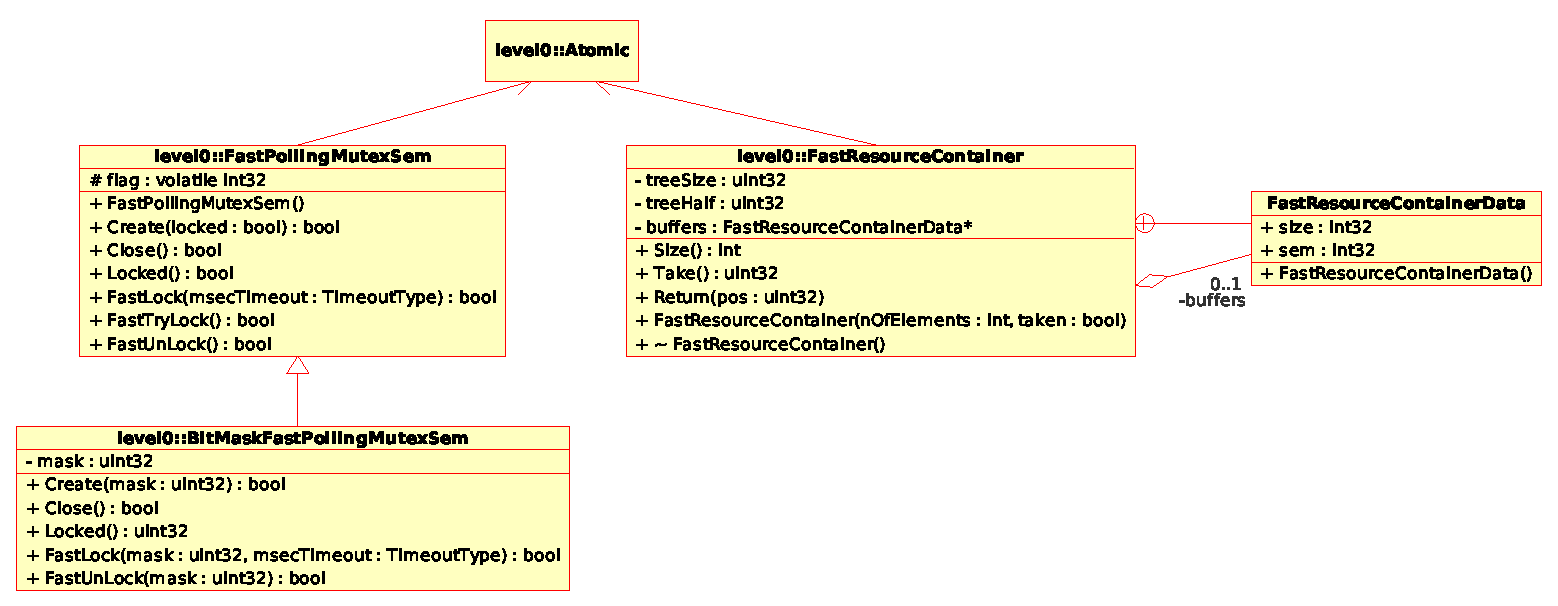
\includegraphics[width=\textwidth]{level0/level0-IPC-Fast.eps}
  \caption{BaseLib Level0 IPC Fast classes}
  \label{f:level0:ipc-fast}
 \end{center}
\end{figure}

Figure \ref{f:level0:ipc-fast} depict spinlock classes in this section (other classes previously anlized are also present: \texttt{Atomic}):

\begin{itemize}
 \item FastPollingMutexSem
 \item BitMaskFastPollingMutexSem
 \item FastResourceContainer
\end{itemize}




\subsubsection{FastPollingMutexSem}
\texttt{[FastPollingMutexSem]}\\
Class \texttt{FastPollingMutexSem} implements a spinlock using atomic test and set operations. Such class can be lock and unlock using also a timeout that is calculated using the \texttt{HRT} class.\\


API naming is quite similar to the \texttt{MutexSem} implementation. The interface is quite simple. \texttt{Create} method initializes the semaphore and reads it; \texttt{Close} undo semaphore initialization. 

The ambiguous named method \texttt{Locked} returns the status of the semaphore.

In this case ``fast'' functions have a meaning infact are the core of this class. \texttt{FastLock} poll the state of the mutex variable at a rate of a one milli seconds until \texttt{msecTimeout} is expired; this is a user space implementation of a spinlock; \texttt{FastTryLock} basically try to achieve the lock one time without waiting; \texttt{FastUnLock} unlock the mutex.

\begin{lstlisting}[
extendedchars=true,%
basicstyle=\fontfamily{pcr}\fontseries{m}\selectfont\footnotesize, %
stepnumber=1,%
numberstyle=\tiny,%
keywordstyle=\footnotesize\tt ,%
language=C++]
public:
   bool Create(bool locked = False);
   bool Close();

   inline bool Locked();

   inline bool FastLock(TimeoutType msecTimeout=TTInfiniteWait);
   inline bool FastTryLock();
   inline bool FastUnLock(void);
\end{lstlisting}

This class is suitable for multiprocessor systems and is the best choice when no OS interference is needed.



\subsubsection{BitMaskFastPollingMutexSem}
\texttt{[BitMaskFastPollingMutexSem.h]}\\
This structure group 32 mutexes, the locked/unlocked state of those mutexes can not be changed interleavedly so a mutex exist to control the access to the shared resource that is the \texttt{uint32} attribute holding the state of all mutexes. This class subclasses the \texttt{FastPollingMutexSem} class requiring it to provide access control to the shared 32 mutex's states.\\


The \texttt{mask} argument in the following methods is required to identify which of the 32 mutexes we want deal with.

\begin{lstlisting}[
extendedchars=true,%
basicstyle=\fontfamily{pcr}\fontseries{m}\selectfont\footnotesize, %
stepnumber=1,%
numberstyle=\tiny,%
keywordstyle=\footnotesize\tt ,%
language=C++]
private:
    uint32 mask;
public:
   bool Create(uint32 mask=0);
   bool Close();

   inline uint32 Locked();

   inline bool FastLock(uint32 mask,TimeoutType msecTimeout=TTInfiniteWait);
   inline bool FastUnLock(uint32 mask);
\end{lstlisting}



\subsubsection{FastResourceContainer}
\texttt{[FastResourceContainer.h]}\\
The class \texttt{FastResourceContainer} is basically an array data structure that if associated to a pool of resource give you the state of each resource. This means that let's for example that you have a pool of N \texttt{int}s in an array that goes from index 0 to index N-1, so you need one of them but without taking care of the index; this could be the condition when multiple entity concurrently need the same type of resource. In this situation you want to ask for a resource and take it without waiting and whitout OS's intervention.
A \texttt{FastResourceContainer} is the key in this situation, it doesn't allocate space buffer for you but can take care of which element of your pool are in use and which are not in use, answering for resource in a time O(n log n). If the pool has no resource your request simply fails. An example application will follow. \\


This mechanism can be imaged as a counting semaphore, independent from the OS because relies only on atomic hardware operations, so can be used between processes, threads, interrupt context on different processors in the mean time returning always immediate (without delay) in a bounded time (real time). \\


The class relay on a nested defined class \texttt{FastResourceContainerData} that take account of the usage state of each controlled resource.
The constructor take care on how many resource do you want to control, \texttt{Size} return the same number; \texttt{Take} return the index of a free resource and \texttt{Return} let you returning a resource index to the system.

\begin{lstlisting}[
extendedchars=true,%
basicstyle=\fontfamily{pcr}\fontseries{m}\selectfont\footnotesize, %
stepnumber=1,%
numberstyle=\tiny,%
keywordstyle=\footnotesize\tt ,%
language=C++]
private:
   uint32 treeSize;
   uint32 treeHalf;

   FastResourceContainerData* buffers;
public:
   FastResourceContainer(int nOfElements,bool taken=False);
   virtual ~FastResourceContainer();

   inline int Size();

   inline uint32 Take();
   inline void Return(uint32 pos);
\end{lstlisting}

Then follow an illustrative example on how to use a \texttt{FastResourceContainer}. In this example we create a buffer memory pool, this buffer memory pool can be used in multiprocessor and in multiple context in the same time thanks to the \texttt{FastResourceContainer}.

\begin{lstlisting}[
extendedchars=true,%
basicstyle=\fontfamily{pcr}\fontseries{m}\selectfont\footnotesize, %
stepnumber=1,%
numberstyle=\tiny,%
keywordstyle=\footnotesize\tt ,%
language=C++]
class DynamicPool: protected FastResourceContainer {
   int size;
   char* ptrBuffer;
public:
   DynamicPool(unsigned int size, int nOfElements, bool taken=False) {
      if (!(size)) size = 1;
      FastResourceContainer(nOfElements, taken);
      ptrBuffer = new char[size*nOfElements];
      this->size = size;
   }
   virtual ~DynamicPool() {
      if (ptrBuffer) delete ptrBuffer;
   }
   int alloc(char*& address) {
      int handle = (int)Take();
      if (handle == -1) return -1;
      address = ptrBuffer + (char*)(size*handle);
      return handle;
   }
   bool free(int handle) {
      return Return((unsigned int)handle);
   }
};
\end{lstlisting}



\subsection{Design Notes}

The \textit{SemNameDataBase} is used in every installation where the OS's libraies doesn't supply the named semaphore abstraction.
Some problems with semaphores are stated in the text; one big implementation problem is the static casting. Static casting is usually a bad programming choice, lets take a non skilled programmer: it pass to a function a wrong object without the right attributes but we are using those attributes in the function! What happens? Bugs, bugs and bugs...\\


SemPurger
The \texttt{Found} method is not a well designed method: the class is not associated to a \texttt{LinkedList} so there is no way to know to which sublist the \texttt{found} attribute's value refer.
A bad implementation choice in those classes is the interface of the \texttt{Test} method: is not really the interface but the code, inside the code there is a static cast of the \texttt{data} argument to \texttt{SemInfoDataBits} a \textit{dynamic cast} was probably a better choice to be sure to have some consistency checks in the code. \\


\texttt{SemCore} that probably can be renamed in something like \texttt{InterfaceSem}; such class is quite useless right now holding only an handle to an OS's entity. The usage count in the \textit{SemNameDataBase} is not currently checked against deletion of a semaphore. \\


The ambiguous named method \texttt{FastPollingMutexSem::Locked} returns the status of the semaphore, a better choice for this name could be \texttt{FastPollingMutexSem::isLocked} (?).



\section{Network}
\begin{figure}[h!]
  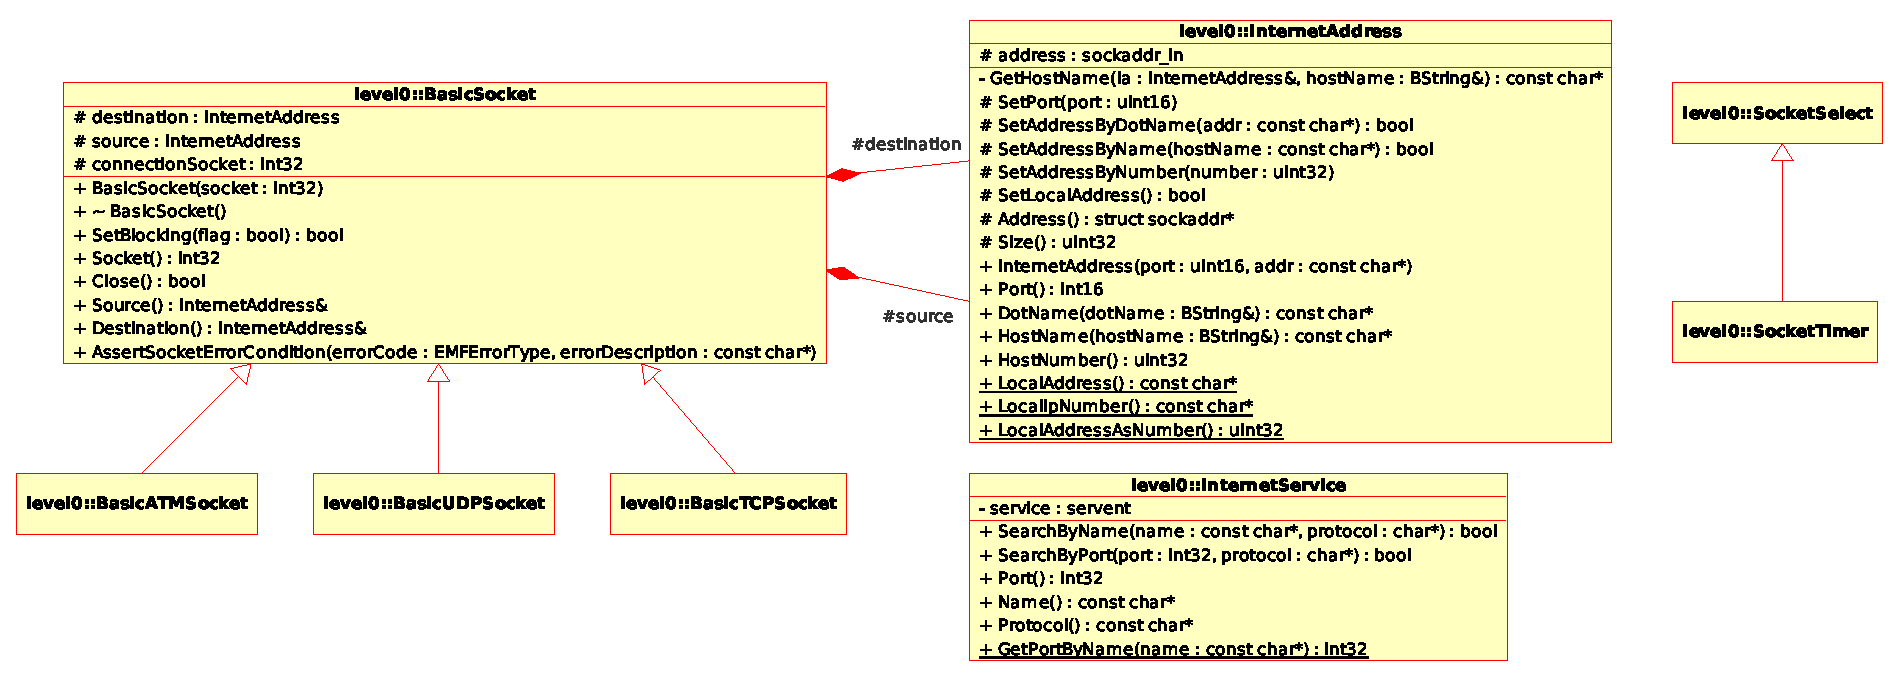
\includegraphics[width=\textwidth]{level0/level0-network.eps}
 \caption{BaseLib Level0 network classes}
 \label{f:level0:network}
\end{figure}

Network classes (Figure \ref{f:level0:network}) at these level inherit from the class \texttt{BasicSocket}. The class \texttt{BasicSocket} treat each source and destination address as a \texttt{InternetAddress} structure. We will start examining such class. \\

Classes in this section:
\begin{itemize}
 \item InternetAddress
 \item InternetService
 \item BasicSocket
 \item BasicATMSocket
 \item BasicTCPSocket
 \item BasicUDPSocket
 \item SocketSelect
 \item SocketTimer
\end{itemize}



\subsubsection{InternetAddress}
\texttt{[InternetAddress.h, InternetAddress.cpp]}\\
Class \texttt{InternetAddress} basically hold the full Internet Protocol version 4.0 (IPv4.0) address (i.e. the IP address and the port number). Right now IPv6.0 is not supported. The class is based on a protected UNIX \texttt{sockaddr\_in} structure.

\begin{lstlisting}[
extendedchars=true,%
basicstyle=\fontfamily{pcr}\fontseries{m}\selectfont\footnotesize, %
stepnumber=1,%
numberstyle=\tiny,%
keywordstyle=\footnotesize\tt ,%
language=C++]
protected:
   sockaddr_in address;
\end{lstlisting}

Setting the IP address is achieved by different functions letting friend classes and subclasses set it by dotted number notation (i.e. 192.168.1.2), name (i.e www.google.co.uk), by 32bit number (i.e. usually in hexadecimal format) and automatically, using the localhost IP; also the port number is not publically settable.

\begin{lstlisting}[
extendedchars=true,%
basicstyle=\fontfamily{pcr}\fontseries{m}\selectfont\footnotesize, %
stepnumber=1,%
numberstyle=\tiny,%
keywordstyle=\footnotesize\tt ,%
language=C++]
protected:
   bool SetAddressByDotName(const char* addr);
   bool SetAddressByName(const char* hostName);
   void SetAddressByNumber(uint32 number);
   bool SetLocalAddress();

   void SetPort(uint16 port);
\end{lstlisting}

Next code lines completes class's interface; the constructor take the port number and the IP in a suitable format to be given in input at the  \texttt{inet\_addr} POSIX API; such function use the numbers-and-dots notation. Public methods let the user only get the IP in different formats, public methods don't allow a user to modify the IP and port number the class holds.

\begin{lstlisting}[
extendedchars=true,%
basicstyle=\fontfamily{pcr}\fontseries{m}\selectfont\footnotesize, %
stepnumber=1,%
numberstyle=\tiny,%
keywordstyle=\footnotesize\tt ,%
language=C++]
   struct sockaddr *Address();
   uint32 Size();
public:
   InternetAddress(uint16 port=0,const char* addr=NULL);

   int16 Port();
   uint32 HostNumber();
   static const char* LocalAddress();
   static const char* LocalIpNumber();
   static uint32 LocalAddressAsNumber();
\end{lstlisting}

The last two functions use the special \texttt{BString} buffer class also defined in directory \textit{level0}. The function \texttt{DotName}
returns the host name in numbers-and-dots notation the returned \texttt{const char*} is a pointer to the \texttt{BString} buffer; the function \texttt{HostName} returns the host name (as a pointer to the BString buffer) by querying the name server, NULL means failure.

\begin{lstlisting}[
extendedchars=true,%
basicstyle=\fontfamily{pcr}\fontseries{m}\selectfont\footnotesize, %
stepnumber=1,%
numberstyle=\tiny,%
keywordstyle=\footnotesize\tt ,%
language=C++]
   const char* DotName(BString &dotName);
   const char* HostName(BString &hostName);
\end{lstlisting}



\subsubsection{BasicSocket}
\texttt{[BasicSocket.h, BasicSocket.cpp]}\\
This class implements generic socket functions. The socket abstraction require to specify an \texttt{InternetAddress} destination and a source. Socket is an abstraction that comes from POSIX standars; using the \textit{libc} library, each opened socket, like each opened file in a program, has associated a unique integer.

\begin{lstlisting}[
extendedchars=true,%
basicstyle=\fontfamily{pcr}\fontseries{m}\selectfont\footnotesize, %
stepnumber=1,%
numberstyle=\tiny,%
keywordstyle=\footnotesize\tt ,%
language=C++]
protected:
   InternetAddress destination;
   InternetAddress source;
   int32           connectionSocket;
\end{lstlisting}

This class is an abstract class defining only the concept behind Sockets: it defines three basic attributes but doesn't implements methods to set or get those attributes, this is not absolutely true but for example you can get the \texttt{destination} and \texttt{source} address but not set. The constructor require a socket identifier, so this class doesn't create a socket for you, is the user that have to first create a socket and than associate a classes to such socket.

\begin{lstlisting}[
extendedchars=true,%
basicstyle=\fontfamily{pcr}\fontseries{m}\selectfont\footnotesize, %
stepnumber=1,%
numberstyle=\tiny,%
keywordstyle=\footnotesize\tt ,%
language=C++]
public:
   BasicSocket(int32 socket = 0);

   bool SetBlocking(bool flag);
   int32 Socket();
   bool Close();
   InternetAddress& Source();
   InternetAddress& Destination();

   void AssertSocketErrorCondition(EMFErrorType errorCode,const char* errorDescription=NULL,...);
   void AssertSocketErrorCondition(EMFErrorType errorCode,const char* errorDescription=NULL,...);
\end{lstlisting}

Last two lines implement error handling for the first time. The enumerated type \texttt{EMFErrorType} follows in the section Exceptions in this chapter; \texttt{errorCode} is a number identifying the type of error not the dangerous level of the error.



\subsubsection{BasicATMSocket}
\texttt{[BasicATMSocket.h, BasicATMSocket.cpp]}\\
This class is one of the three subclasses of the \texttt{BasicSocket} class. Basically it adds the support to ATM socket at AAL5 protocol. An ATM network is not socket oriented but it relay on channels (Virtual Circuits). Unix developer try to uniformly this kind of network letting ATM network users using the same socket abstraction used for connection oriented protocols.

The most important information regarding a Virtual Circuit is the Virtual Circuit Index (VCI).

\begin{lstlisting}[
extendedchars=true,%
basicstyle=\fontfamily{pcr}\fontseries{m}\selectfont\footnotesize, %
stepnumber=1,%
numberstyle=\tiny,%
keywordstyle=\footnotesize\tt ,%
language=C++]
protected:
   uint32 VCI;
\end{lstlisting}

This code use the POSIX interface to write and read to an ATM network card. Core functions to read or write are private and are declared as follow. This solution is adopted to let a set of friends function calling the methods have access to protected attributes of \texttt{InternetAddress}. A C interface that use the object is given.

\begin{lstlisting}[
extendedchars=true,%
basicstyle=\fontfamily{pcr}\fontseries{m}\selectfont\footnotesize, %
stepnumber=1,%
numberstyle=\tiny,%
keywordstyle=\footnotesize\tt ,%
language=C++]
private:
   bool _Read(const void* buffer,uint32& size,TimeoutType msecTimeout);
   bool _Write(const void* buffer,uint32& size,TimeoutType msecTimeout);
\end{lstlisting}

Like a \texttt{BasicSocket} the constructor doesn't create a socket but it is the user that must supply a newly created socket for the constructor. Using the \texttt{Open} method it is possible to open a new ATM socket without passing it via the constructor, \texttt{SetVCI} and \texttt{GetVCI} let's setting and getting the Virtual Channel Index (a number).

The \texttt{Read} and \texttt{Write} function reads and writes a block of data, \texttt{size} is the maximum size in bytes of the required transfer for a write operation; during a read \texttt{size} holds first the maximum buffer size and after the read the readed size in bytes. Timeout is currently not supported.

\begin{lstlisting}[
extendedchars=true,%
basicstyle=\fontfamily{pcr}\fontseries{m}\selectfont\footnotesize, %
stepnumber=1,%
numberstyle=\tiny,%
keywordstyle=\footnotesize\tt ,%
language=C++]
public:
   BasicATMSocket(int32 socket);

   bool Open();
   inline bool Read(void* buffer, uint32& size, TimeoutType msecTimeout=TTDefault);
   inline bool Write(const void* buffer, uint32& size, TimeoutType msecTimeout=TTDefault);
   inline bool SetVCI(int32 VCI);
   inline uint32 GetVCI();
\end{lstlisting}

To use an ATM oriented channel using such class interface it is necessary to follow those steps, in that order:
\begin{enumerate}
 \item create a brand new \texttt{BasicATMSocket} object;
 \item call method \texttt{Open} on the object;
 \item call method \texttt{SetVCI} on the object;
 \item now it is possible to read and wirte on the object.
\end{enumerate}



\subsubsection{BasicTCPSocket}
\texttt{[BasicTCPSocket.h]}\\
Implements general TCP/IP stream-sockets. All methods implemented in this class are public, no private attribute or method. There are three IO functions: one to write on the stream and two to read from, the second, \texttt{Peek} doesn't consume what it reads.

\begin{lstlisting}[
extendedchars=true,%
basicstyle=\fontfamily{pcr}\fontseries{m}\selectfont\footnotesize, %
stepnumber=1,%
numberstyle=\tiny,%
keywordstyle=\footnotesize\tt ,%
language=C++]
public:
   bool BasicWrite(const void* buffer, uint32& size);
   bool BasicRead(void* buffer, uint32& size);
   bool Peek(void* buffer, uint32& size);
\end{lstlisting}

The constructor take as an argument a socket. If you doesn't want to supply a socket the function \texttt{Open} create one for you. \texttt{Listen} functions bind the socket on a given port number for incoming connections, the function \texttt{WaitConnection} return \texttt{BasicTCPSocket*} on newly estabilished connection on the binded socket.
\texttt{Connect} functions let the user connect to some other remote or local sockets.

\begin{lstlisting}[
extendedchars=true,%
basicstyle=\fontfamily{pcr}\fontseries{m}\selectfont\footnotesize, %
stepnumber=1,%
numberstyle=\tiny,%
keywordstyle=\footnotesize\tt ,%
language=C++]
   BasicTCPSocket(int32 socket = 0);
   bool Open();

   bool Listen(int port,int maxConnections=1);
   bool Listen(char *serviceName,int maxConnections=1);
   BasicTCPSocket* WaitConnection(TimeoutType msecTimeout=TTInfiniteWait,
      BasicTCPSocket* client=NULL);

   bool Connect(const char* address,int port,TimeoutType msecTimeout=TTInfiniteWait);
   bool Connect(const char* address,const char* serviceName,
      TimeoutType msecTimeout=TTInfiniteWait);
   bool IsConnected();
\end{lstlisting}

This interface permit to specify ports as a number or as a service name (string) this is achieved using the \texttt{InternetService::GetPortByName} facility. The \texttt{InternetService} interface is reported here:

\begin{lstlisting}[
extendedchars=true,%
basicstyle=\fontfamily{pcr}\fontseries{m}\selectfont\footnotesize, %
stepnumber=1,%
numberstyle=\tiny,%
keywordstyle=\footnotesize\tt ,%
language=C++]
class InternetService {
   servent service;
public:
   bool SearchByName(const char* name,char* protocol=NULL);
   bool SearchByPort(int32 port,char* protocol=NULL);
   int32 Port();
   const char* Name();
   const char* Protocol();
   static int32 GetPortByName(const char* name);
};
\end{lstlisting}



\subsubsection{BasicUDPSocket}
\texttt{[BasicUDPSocket.h]}\\
Implements a general UDP/IP socket. UDP protocol is connectionless and so differently from TCP doesn't need a connection, the \texttt{BasicUDPSocket} class implements also the \texttt{Connect} function that is used to select the destination of the next sends; infact using the IO function below is not possible to choose a destination address. Every message received on the selected UDP port is received.

\begin{lstlisting}[
extendedchars=true,%
basicstyle=\fontfamily{pcr}\fontseries{m}\selectfont\footnotesize, %
stepnumber=1,%
numberstyle=\tiny,%
keywordstyle=\footnotesize\tt ,%
language=C++]
public:
   bool BasicRead(void* buffer, uint32& size);
   bool BasicWrite(const void* buffer, uint32& size);
\end{lstlisting}

As usual the constructor let you create an object using a previous opened UDP socket or create a brand new socket with the \texttt{Open} method.

\begin{lstlisting}[
extendedchars=true,%
basicstyle=\fontfamily{pcr}\fontseries{m}\selectfont\footnotesize, %
stepnumber=1,%
numberstyle=\tiny,%
keywordstyle=\footnotesize\tt ,%
language=C++]
   BasicUDPSocket(int32 socket = 0);
   bool Open();

   bool Listen(int port,int maxConnections=1);
   bool Connect(const char *address,int port);
   bool Connect(InternetAddress &dest);
\end{lstlisting}



\subsubsection{SocketSelect}
\texttt{[SocketSelect.h]}\\
This class provide a wrapper to the \texttt{select} \textit{libc} function allowing the synchronization of a group of sockets. This stuff can only select sockets from a single source type, is not allowed to mix ATM and UDP on NT platforms.

\begin{lstlisting}[
extendedchars=true,%
basicstyle=\fontfamily{pcr}\fontseries{m}\selectfont\footnotesize, %
stepnumber=1,%
numberstyle=\tiny,%
keywordstyle=\footnotesize\tt ,%
language=C++]
protected:
   fd_set readFDS;
   fd_set writeFDS;
   fd_set exceptFDS;
   fd_set readFDS_done;
   fd_set writeFDS_done;
   fd_set exceptFDS_done;
   int32 readySockets;

public:
   SocketSelect();

   void Reset();
   void AddWaitOnWriteReady(BasicSocket* s);
   void DeleteWaitOnWriteReady(BasicSocket* s);
   void AddWaitOnReadReady(BasicSocket* s);
   void DeleteWaitOnReadReady(BasicSocket* s);
   void AddWaitOnExceptReady(BasicSocket* s);
   void DeleteWaitOnExceptReady(BasicSocket* s);

   bool Wait(TimeoutType msecTimeout=TTInfiniteWait);
   bool WaitRead(TimeoutType msecTimeout=TTInfiniteWait);
   bool WaitWrite(TimeoutType msecTimeout=TTInfiniteWait);
   bool WaitExcept(TimeoutType msecTimeout=TTInfiniteWait);

   int32 ReadySockets();
   bool CheckRead(BasicSocket* s);
   bool CheckWrite(BasicSocket* s);
   bool CheckExcept(BasicSocket* s);
   fd_set& ReadFDS();
   fd_set& WriteFDS();
   fd_set& ExceptFDS();
\end{lstlisting}



\subsubsection{SocketTimer}
\texttt{[SocketTimer.h]}\\
To simplify some use of select; this is a tool to specify a maximum wait on socket actions. The interface is quite simple. The most important thing is the time attribute \texttt{timeWait} that model the time to wait in a timeout operation.
It is possible to wait for a \textit{read} or \textit{write} operation.

\begin{lstlisting}[
extendedchars=true,%
basicstyle=\fontfamily{pcr}\fontseries{m}\selectfont\footnotesize, %
stepnumber=1,%
numberstyle=\tiny,%
keywordstyle=\footnotesize\tt ,%
language=C++]
private:
   timeval timeWait;

public:
   void SetMsecTimeout(TimeoutType msecTimeout=TTInfiniteWait);
   bool WaitRead();
   bool WaitWrite();
   uint32 MSecTimeout();
\end{lstlisting}



\subsection{Design Notes}

Sockets are a powerfull abstraction due to UNIX operating system. The construction adopted here is quite general and is fully compatible with many operating systems on the market. \\


Probably further code to support newer protocol like IPv6.0 is needed in the future. The class diagram using the class developed require that all the system relay on IP, that is not true for ATM networks, it lacks some generality. \\


Too many code inlining is not ever a good design choice: systems with low memory constraints will became fast a difficult target to support. Code inlining produce many copy of the same code in the library.\\



\section{Files, Streams}
This section groups togheter two basic concepts: files and streams. For each concepts there is a subsection. There are only few classes involved in this group.
If you see Files and Streams implementations you can note that the interface is quite similar between \texttt{BasicFile} and \texttt{StreamInterface}.



\subsection{Files}
Files abstraction come from UNIX OSes and are nowadays the principal abstraction for data storage. BaseLib's file classes are depicted in Figure \ref{f:level0:file}; there are only two classes, without any link, as listed below:
\begin{itemize}
 \item BasicFile
 \item BasicConsole
\end{itemize}

\begin{figure}[h!]
 \begin{center}
  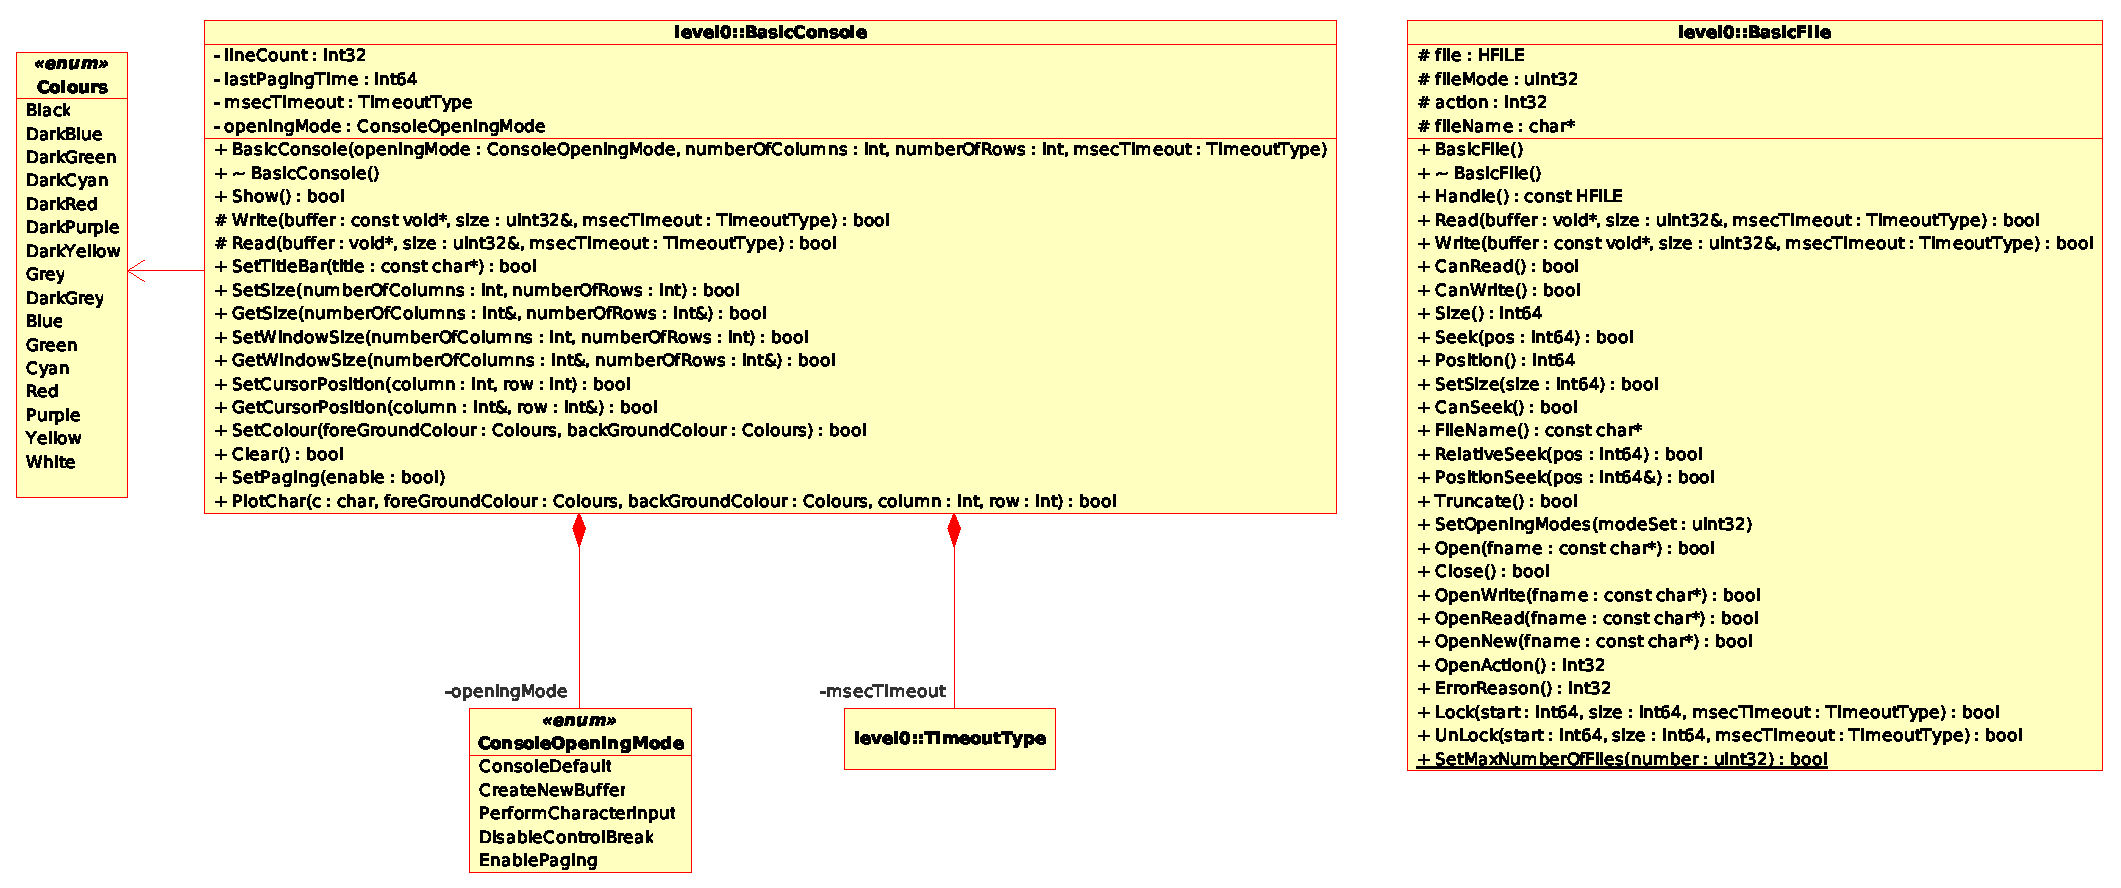
\includegraphics[width=\textwidth]{level0/level0-file.eps}
  \caption{BaseLib Level0 file classes}
  \label{f:level0:file}
 \end{center}
\end{figure}

Classes methods are quite similar, this is why they are grouped together, a Console or better a terminal, is in UNIX treated as a file with a more special interface support to terminal (see \texttt{man termios}). Infact during the past there were a great use of serial link and a serial link let computer dial togheter, a serial link in a UNIX system is a file and so a serial device is a file ( as an example \texttt{/dev/ttys0}) serial link has some special character (or set of it) that let the user treat it as a terminal so the UNIX developer introduced those special function as extended functions of a file abstraction. Infact in UNIX a Console can also be locked but in BaseLib no.



\subsubsection{BasicFile}
\texttt{[BasicFile.h, BasicFile.cpp]}\\
The \texttt{BasicFile} class is istantiated per opened file the basic information carried from the class is a \texttt{HFILE} handle to the file, a mode mask that can be queried to know if the file was opened in write or read only mode (\texttt{fileMode}), an \texttt{int32} attribute (\texttt{action)} used to hold an error code in case of failure and the file name (\texttt{fileName}).

\begin{lstlisting}[
extendedchars=true,%
basicstyle=\fontfamily{pcr}\fontseries{m}\selectfont\footnotesize, %
stepnumber=1,%
numberstyle=\tiny,%
keywordstyle=\footnotesize\tt ,%
language=C++]
protected:
   HFILE file;
   uint32 fileMode;
   int32 action;
   char* fileName;
\end{lstlisting}

There is only one protected method \texttt{SetFileName} that let the developer of subclasses to change the file's name. The class constructor doesn't require any parameters.\\


Basic \textit{get} methods are \texttt{Handle} that return the OS related file handle (an integer in UNIX); \texttt{FileName} return the name of the file and \texttt{Size} return the size of the file object. The method \texttt{SetSize} lets you set the file size by either truncating or extending the file size. The only static method, \texttt{SetMaxNumberOfFiles} try to set a Operating System wide parameter of the maximum number of files opened in the system, in VxWorks it simply return \texttt{true}.

\begin{lstlisting}[
extendedchars=true,%
basicstyle=\fontfamily{pcr}\fontseries{m}\selectfont\footnotesize, %
stepnumber=1,%
numberstyle=\tiny,%
keywordstyle=\footnotesize\tt ,%
language=C++]
   void SetFileName(const char* name);
public:
   const HFILE Handle();
   inline const char* FileName();

   inline int64 Size();
   inline bool SetSize(int64 size);

   static inline bool SetMaxNumberOfFiles(uint32 number);
\end{lstlisting}

Before opening a file the first action to do is to set the file opening modes with the \texttt{SetOpeningModes}, opening modes are listed in the firt 50's row of the file \textit{level0/BasicFile.h}. Then it is possible to open a file with the method \texttt{Open}. To avoid the burden of making two calls it is possible to use the methods \texttt{OpenWrite} \texttt{OpenRead} \texttt{OpenNew} to open for write, open read only and create a file. If during an open operation happen something unexpected it's possible to query about what happens with the \texttt{OpenAction} and \texttt{ErrorReason} methods.

\begin{lstlisting}[
extendedchars=true,%
basicstyle=\fontfamily{pcr}\fontseries{m}\selectfont\footnotesize, %
stepnumber=1,%
numberstyle=\tiny,%
keywordstyle=\footnotesize\tt ,%
language=C++]
   inline void SetOpeningModes(uint32 modeSet);
   bool Open(const char *fname,...);
   inline bool Close();

   bool OpenWrite(const char *fname,...);
   bool OpenRead(const char *fname,...);
   bool OpenNew(const char *fname,...);

   inline int32 OpenAction();
   int32 ErrorReason();
\end{lstlisting}

The \texttt{Read} and \texttt{Write} operation have a timeout to stop blocking the caller processor. The functions have the same interface, the size in each case is readed and written so its an in/out argument. Query methods \texttt{CanRead} and \texttt{CanWrite} parse the attribute \texttt{fileMode} to understand with which options the file was opened. There is no way to understand if the file was just opened or newer opened.

\begin{lstlisting}[
extendedchars=true,%
basicstyle=\fontfamily{pcr}\fontseries{m}\selectfont\footnotesize, %
stepnumber=1,%
numberstyle=\tiny,%
keywordstyle=\footnotesize\tt ,%
language=C++]
   inline bool Read(void* buffer, uint32& size, TimeoutType msecTimeout=TTDefault);
   inline bool Write(const void* buffer, uint32& size, TimeoutType msecTimeout=TTDefault);
   inline bool CanRead();
   inline bool CanWrite();
\end{lstlisting}

For random file access BaseLib supplies \texttt{Position} method to know the current file position; with the \texttt{CanSeek} method it possible to query regarding the capability of seeking a file (basically an OS's dependent task). Seeking a file is easily obtained using \texttt{Seek} to move to a specific absolute position (i.e. the position is expressed from the beginning of the file), \texttt{PositionSeek} method behave in the same way but the \texttt{pos} is an in/out argument; if you require to move to a relative position simply use \texttt{RelativeSeek}.\\


The method \texttt{Truncate} clip the file size to the current seek point (i.e. the current position). The last two function let the user lock and unlock to the application the access of the file region starting from \texttt{start} and \texttt{size} bytes long. If it was locked wait as much as timeout.

\begin{lstlisting}[
extendedchars=true,%
basicstyle=\fontfamily{pcr}\fontseries{m}\selectfont\footnotesize, %
stepnumber=1,%
numberstyle=\tiny,%
keywordstyle=\footnotesize\tt ,%
language=C++]
   inline int64 Position(void);

   inline bool CanSeek();
   inline bool Seek(int64 pos);
   inline bool PositionSeek(int64 &pos);
   inline bool RelativeSeek(int64 pos);

   inline bool Truncate();

   inline bool Lock(int64 start,int64 size,TimeoutType msecTimeout = TTInfiniteWait);
   inline bool UnLock(int64 start,int64 size,TimeoutType msecTimeout = TTInfiniteWait);
\end{lstlisting}



\subsubsection{BasicConsole}
\texttt{[BasicConsole.h, BasicConsole.cpp]}\\
As stated before a \textit{console} can be treated as a \textit{file} entity but in BaseLib are completely separated but there are some common methods with the same signature. An example of a console in Microsoft Windows$^{\copyright}$ is the Command Prompt in Linux and other UNIX systems you can experienced differents sort of consoles. \\


Attributes start with some OS's handle different from OS to OS, below are cut and pasted only Window's and Linux's handles. \texttt{lineCount} count how many lines since last paging and \texttt{lastPagingTime} how long since last paging; \texttt{msecTimeout} represents how long to wait when reading on the console, \texttt{openingMode} sets of flags describing the console status.

\begin{lstlisting}[
extendedchars=true,%
basicstyle=\fontfamily{pcr}\fontseries{m}\selectfont\footnotesize, %
stepnumber=1,%
numberstyle=\tiny,%
keywordstyle=\footnotesize\tt ,%
language=C++]
#if defined (_WIN32)
   HANDLE inputConsoleHandle;
   HANDLE outputConsoleHandle;
#elif defined (_LINUX)
   struct termio originalConsoleModes;
#endif
   int32 lineCount;
   int64 lastPagingTime;
   TimeoutType msecTimeout;
   ConsoleOpeningMode openingMode;
\end{lstlisting}

The constructor takes four arguments: the first is of type \texttt{ConsoleOpeningMode}, an \texttt{enum} (defined in \textit{level0/BasciConsole.h}) that defines how to open the console (can be an orred combination); the second and the third arguments define respectively the number of columns and rows of the opened console; the last argument is a timeout that update the attribute \texttt{msecTimeout}.
\texttt{Show} simply try to show the console; basically it call an OS's API.

Protected methods let a subclass to write and read to the console; only a subclass is able to make IO operations on a \texttt{BasicConsole} this require to extend a \texttt{BasicConsole} to have a real working \textit{console}.


\begin{lstlisting}[
extendedchars=true,%
basicstyle=\fontfamily{pcr}\fontseries{m}\selectfont\footnotesize, %
stepnumber=1,%
numberstyle=\tiny,%
keywordstyle=\footnotesize\tt ,%
language=C++]
public:
   BasicConsole(ConsoleOpeningMode openingMode=ConsoleDefault,
      int numberOfColumns=-1,
      int numberOfRows=-1,
      TimeoutType msecTimeout=TTInfiniteWait);
   virtual ~BasicConsole();

   inline bool Show();
protected:
   inline bool Write(const void* buffer,uint32& size,TimeoutType msecTimeout);
   inline bool Read(void* buffer,uint32& size,TimeoutType msecTimeout);
\end{lstlisting}

The following methods are oriented to graphical operating systems were a \textit{console} is usually displayed in a \textit{window}. The first method (\texttt{SetTitleBar}) infact lets you set the title bar text of a console window; \texttt{SetPaging} enable or disable paging in the console window; \texttt{SetColour} sets the font foreground and background colours. Take a look to the \texttt{enum Colours} in Figure \ref{f:level0:file} to see the currently available colours. \\


To set and retrieve the size of the \textit{console buffer} in columns and rows you must use \texttt{SetSize} and \texttt{GetSize}; to set and retrieve the size of the \textit{console window} in columns and rows there are \texttt{SetWindowSize} and \texttt{GetWindowSize}. Last couple of functions is full implemented only in Microsoft Windows$^{\copyright}$. Figure \ref{f:level0:console} explain the differences between the \textit{console window} and \textit{console buffer}.

\begin{figure}[h!]
 \begin{center}
  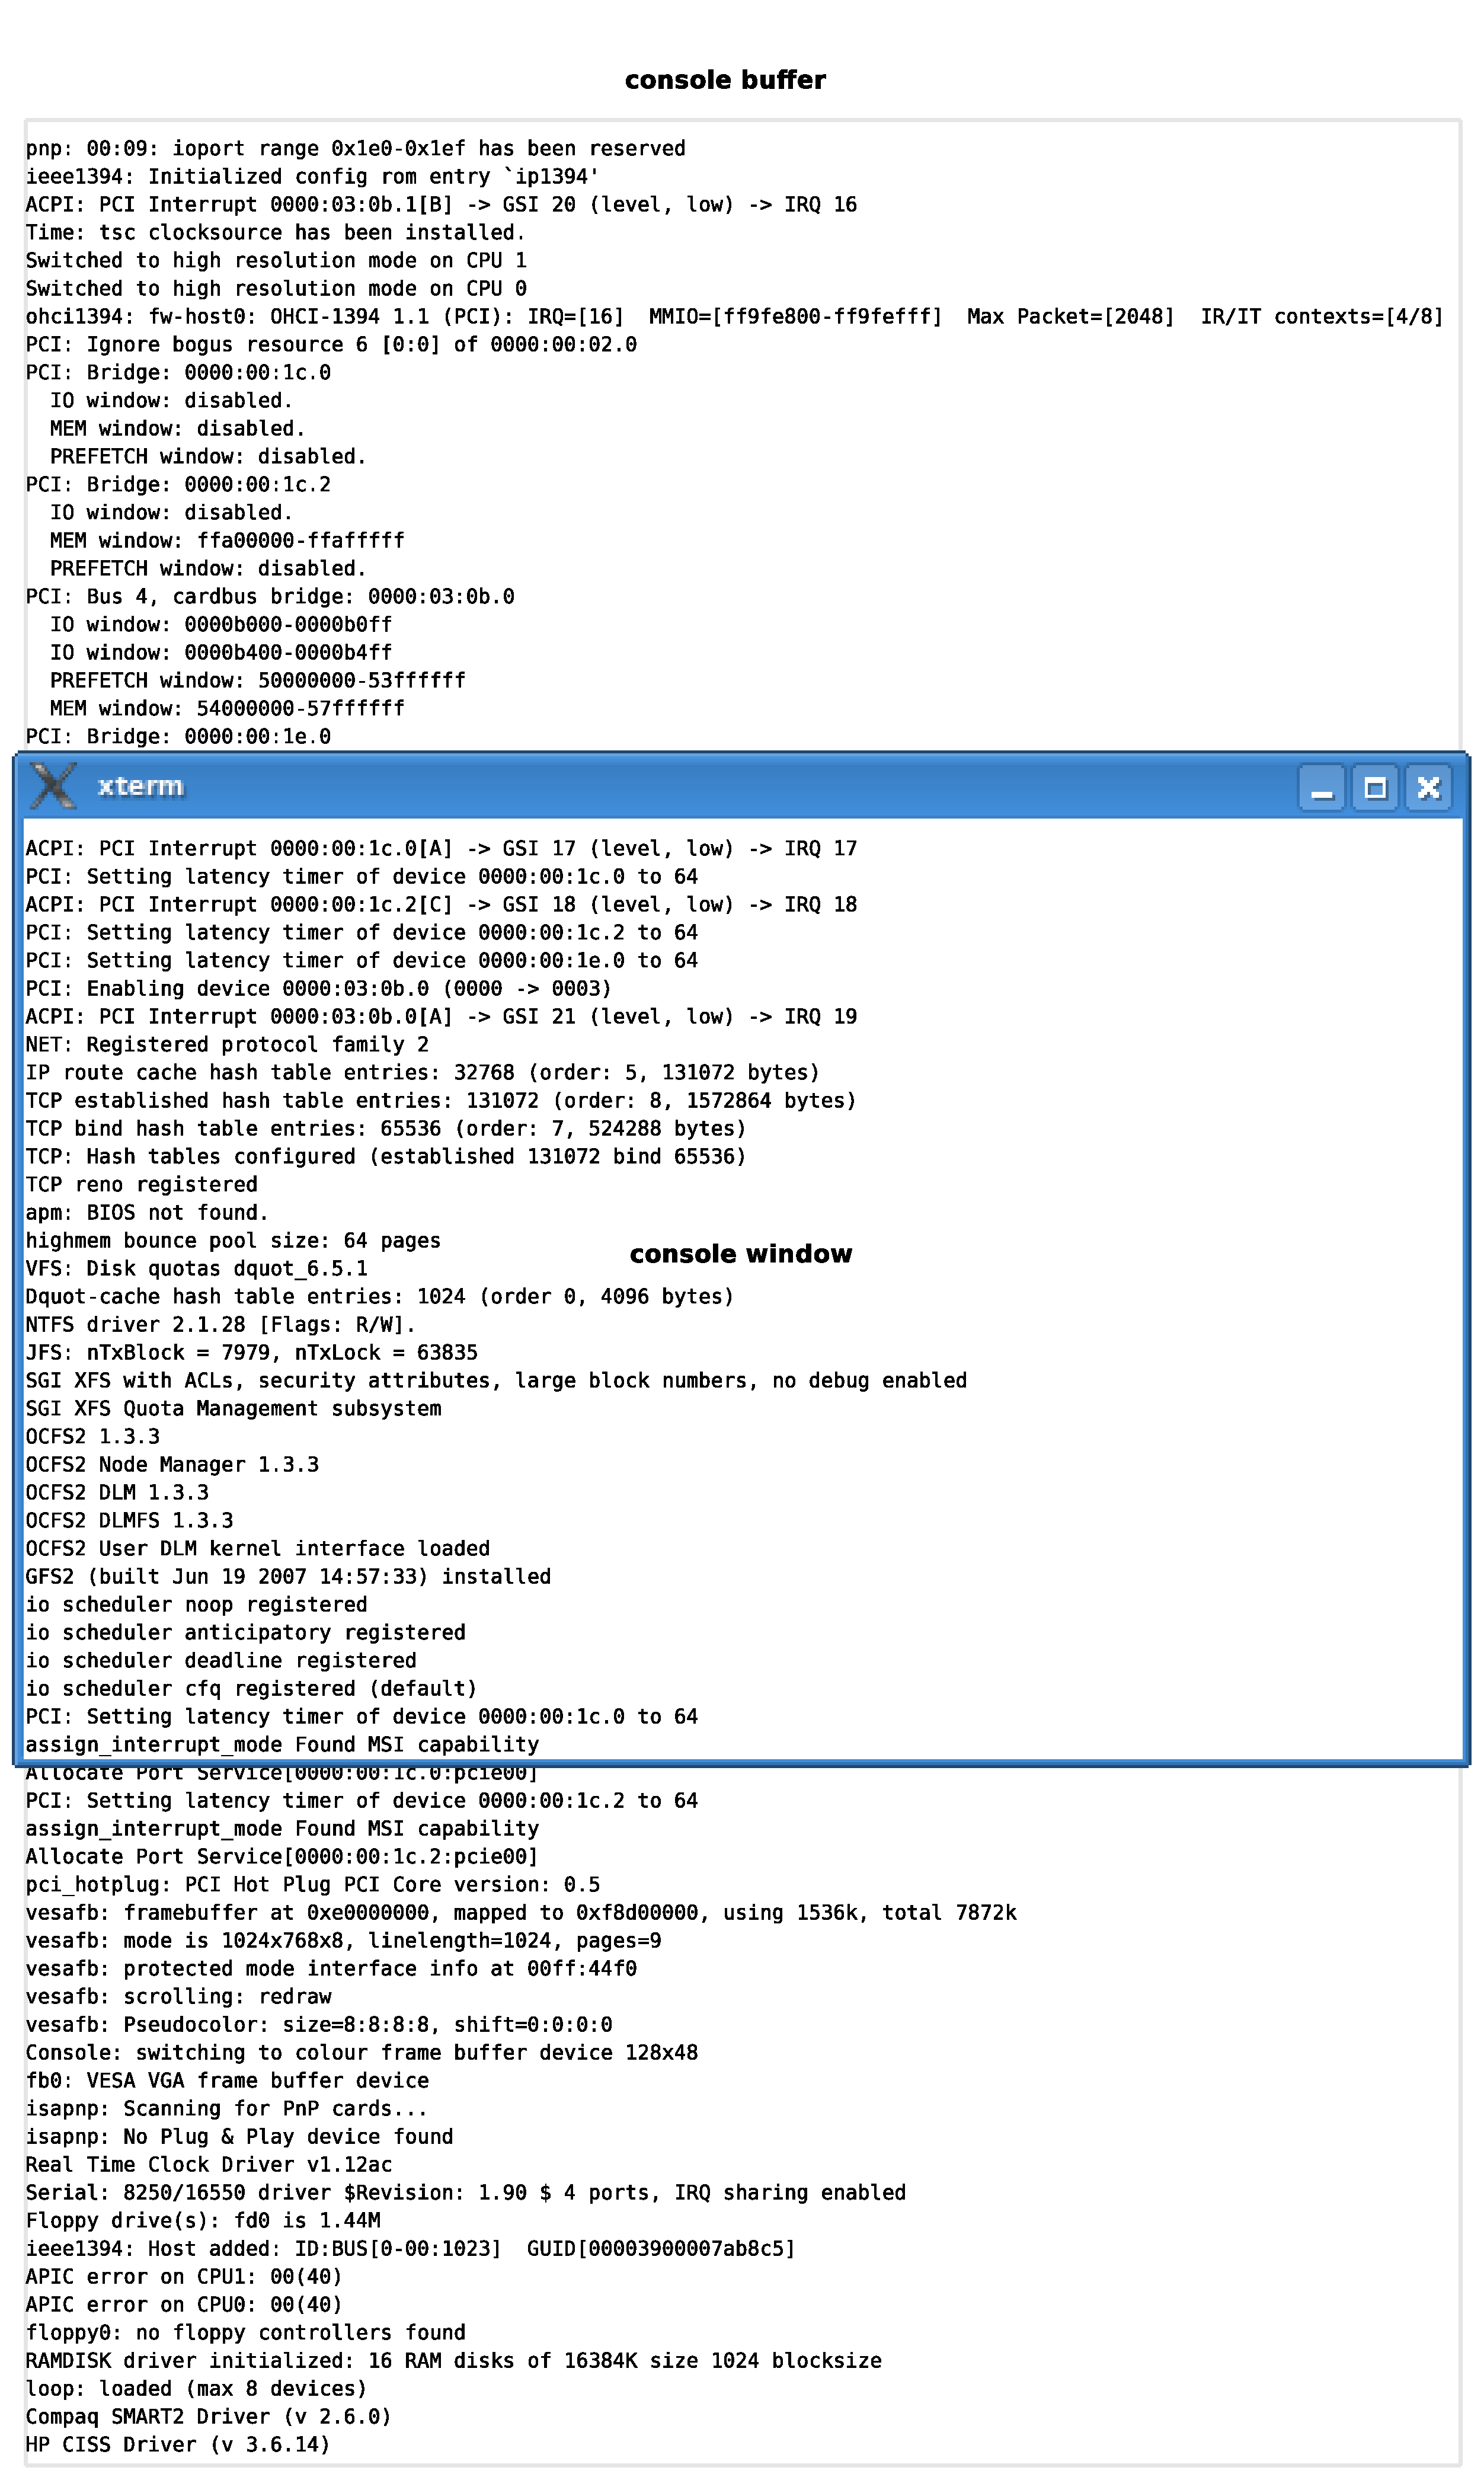
\includegraphics[width=0.49\textwidth]{level0/console.eps}
  \caption{BaseLib console scheme}
  \label{f:level0:console}
 \end{center}
\end{figure}

The method \texttt{SetCursorPosition} sets the position of the cursor in columns and rows; \texttt{GetCursorPosition} retrieve the cursor position. \texttt{Clear} clears the console's content. \texttt{PlotChar} write a single char on the console at a given position and with a given colour set.

\begin{lstlisting}[
extendedchars=true,%
basicstyle=\fontfamily{pcr}\fontseries{m}\selectfont\footnotesize, %
stepnumber=1,%
numberstyle=\tiny,%
keywordstyle=\footnotesize\tt ,%
language=C++]
public:
   inline bool SetTitleBar(const char* title);
   inline void SetPaging(bool enable);
   inline bool SetColour(Colours foreGroundColour,Colours backGroundColour);

   inline bool SetSize(int numberOfColumns,int numberOfRows);
   inline bool GetSize(int& numberOfColumns,int& numberOfRows);

   inline bool SetWindowSize(int numberOfColumns,int numberOfRows);
   inline bool GetWindowSize(int& numberOfColumns,int& numberOfRows);

   inline bool SetCursorPosition(int column, int row);
   inline bool GetCursorPosition(int& column,int& row);

   inline bool Clear();
   inline bool PlotChar(char c,
      Colours foreGroundColour,
      Colours backGroundColour,
      int column, int row);
\end{lstlisting}



\subsection{Streams}
The stream abstraction come from the Object Oriented Design work. C++ defines its standard streams, have a look at \texttt{iostream} and \texttt{fstream} but BaseLib redefine them. In this group of classes we explore the following classes (depicted in Figure \ref{f:level0:stream}):
\begin{itemize}
 \item StreamInterface
 \item PrintfStreamInterface
 \item CStream, CStreamNewBufferFN
\end{itemize}

\begin{figure}[h!]
 \begin{center}
  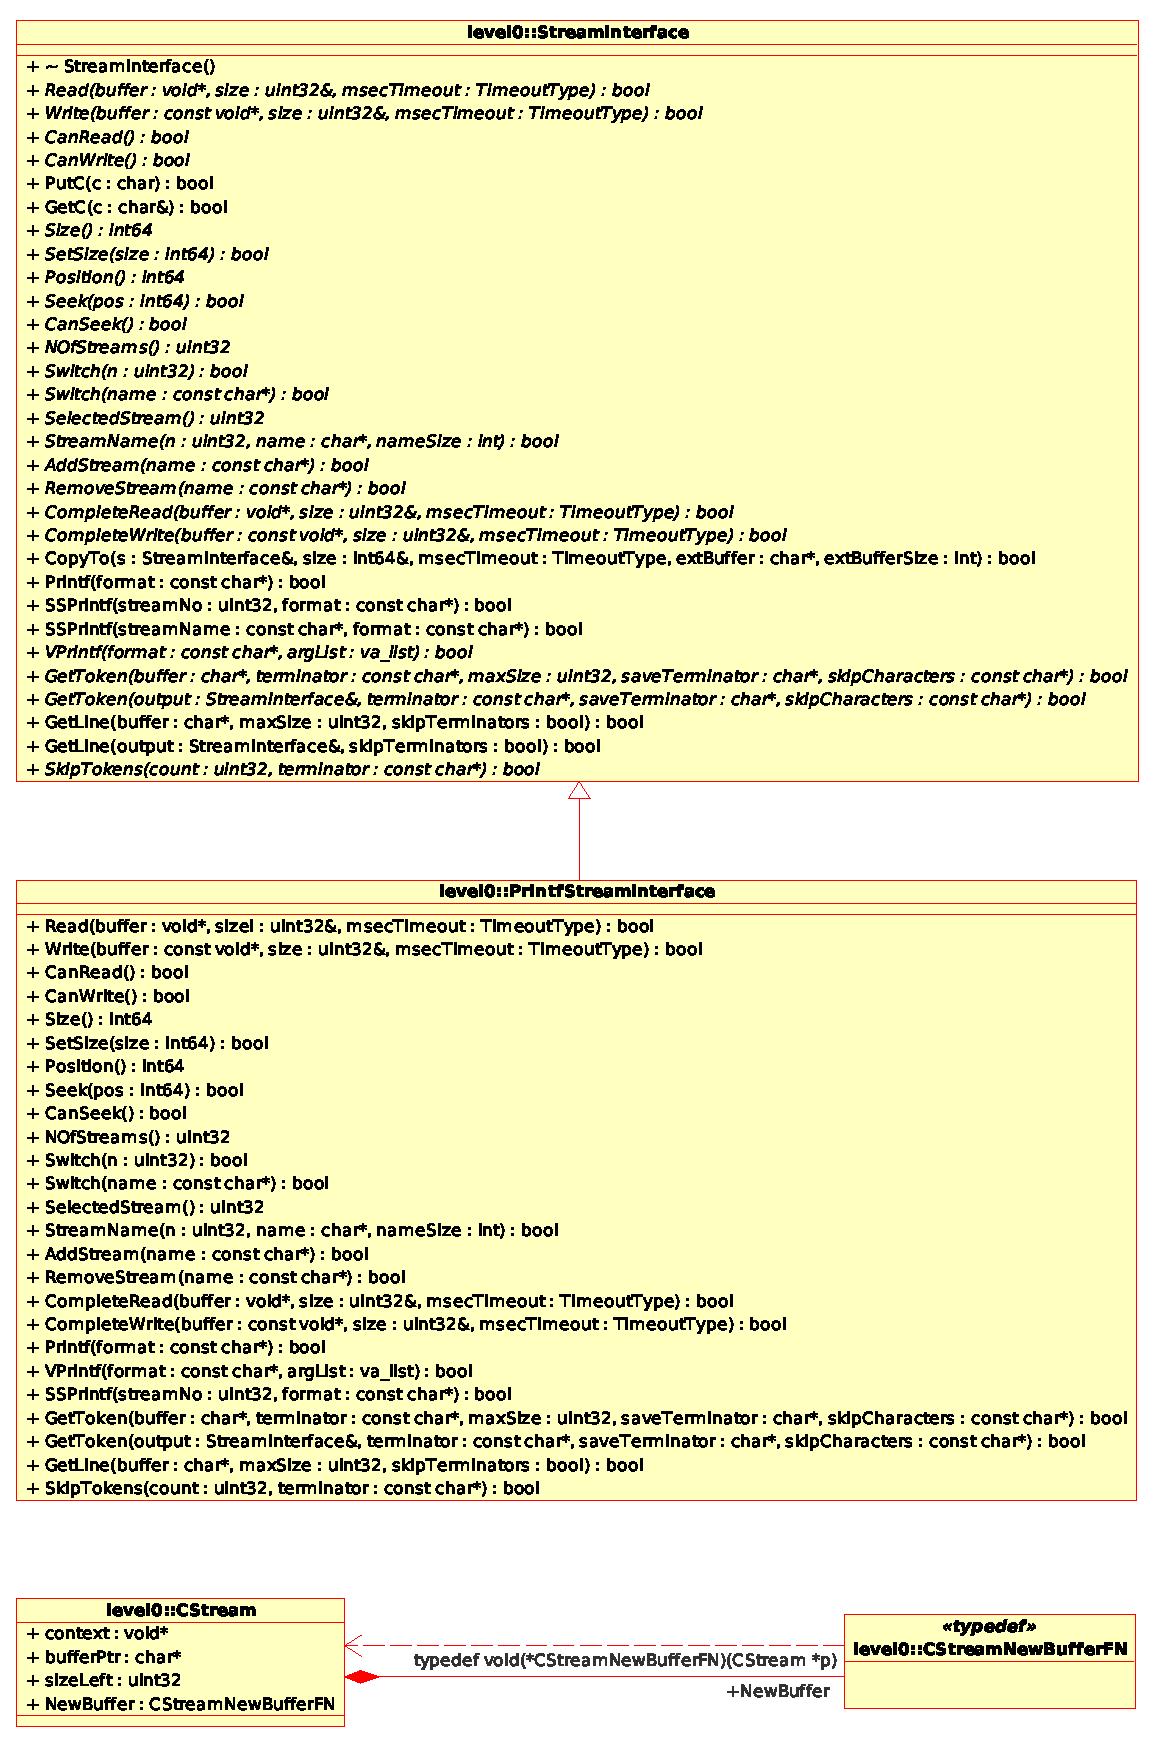
\includegraphics[width=0.57\textwidth]{level0/level0-stream.eps}
  \caption{BaseLib Level0 base stream classes}
  \label{f:level0:stream}
 \end{center}
\end{figure}



\subsubsection{StreamInterface}
\texttt{[StreamInterface.h, StreamInterface.cpp]}\\
The StreamInterface is really important: an entire BaseLib's Level is build on it. Such level focuses on streams defining the \texttt{Streamable} object on top of the \texttt{StreamInterface} that is abstract version. It is used to allow referring to streams at lower levels.
The class has many \textit{pure virtual} methods and a few inline methods so its an abstract C++ class.\\


The method \texttt{Read} reads data into \texttt{buffer} as much as \texttt{size} byte are written, actual size is returned in \texttt{size}; \texttt{msecTimeout} argument is how much the operation should last, timeout behaviour is class specific, i.e. sockets with blocking activated wait forever when \texttt{noWait} is used.
The method \texttt{Write} writes data from \texttt{buffer} to the stream as much as \texttt{size} byte are written, actual size is returned in \texttt{size}, \texttt{msecTimeout} is how much the operation should last; also here timeout behaviour is class specific.

Methods \texttt{CanRead} and \texttt{CanWrite} let you know about the capability to read or write on the stream. \texttt{PutC} implements a single character write operation, \texttt{GetC} implements single character read operation.

\begin{lstlisting}[
extendedchars=true,%
basicstyle=\fontfamily{pcr}\fontseries{m}\selectfont\footnotesize, %
stepnumber=1,%
numberstyle=\tiny,%
keywordstyle=\footnotesize\tt ,%
language=C++]
public:
   virtual bool Read(void* buffer,uint32& size,TimeoutType msecTimeout=TTDefault)=0;
   virtual bool Write(const void* buffer,uint32& size,TimeoutType msecTimeout=TTDefault)=0;

   virtual bool CanRead()=0;
   virtual bool CanWrite()=0;

   inline bool PutC(char c);
   inline bool GetC(char &c);
\end{lstlisting}

The method \texttt{Size} return the size of the stream and \texttt{SetSize} clip the stream size to a specified point (similar to \texttt{Truncate} method). \texttt{Position} returns current position, \texttt{Seek} moves within the file to an absolute location in the file and \texttt{CanSeek} let you query about the capability of seeking.

\begin{lstlisting}[
extendedchars=true,%
basicstyle=\fontfamily{pcr}\fontseries{m}\selectfont\footnotesize, %
stepnumber=1,%
numberstyle=\tiny,%
keywordstyle=\footnotesize\tt ,%
language=C++]
   virtual int64 Size()=0;
   virtual bool SetSize(int64 size)=0;

   virtual int64 Position(void)=0;
   virtual bool Seek(int64 pos)=0;
   virtual bool CanSeek()=0;
\end{lstlisting}

Following methods define a multiple streams interface, \texttt{NOfStreams} return how many streams are available, \texttt{Switch} select the stream to read from, switching may reset the stream to the start, the same method overloaded let the user \texttt{Switch} by name to another stream. \texttt{SelectedStream} return the index of the currently used stream, using \texttt{StreamName} it possible to retrieve also the stream name. Using \texttt{AddStream} you can add a new stream to write to, removing is possible with \texttt{RemoveStream}. Those functions used togheter lets manage streams registration and cancellation.

\begin{lstlisting}[
extendedchars=true,%
basicstyle=\fontfamily{pcr}\fontseries{m}\selectfont\footnotesize, %
stepnumber=1,%
numberstyle=\tiny,%
keywordstyle=\footnotesize\tt ,%
language=C++]
   virtual uint32 NOfStreams()=0;
   virtual bool Switch(uint32 n)=0;
   virtual bool Switch(const char* name)=0;
   virtual uint32 SelectedStream()=0;
   virtual bool StreamName(uint32 n,char* name,int nameSize)=0;
   virtual bool AddStream(const char* name)=0;
   virtual bool RemoveStream(const char* name)=0;
\end{lstlisting}

The method \texttt{CompleteRead} performs the job of a \texttt{Read} function but gurantees the completion; in case of failure \texttt{size} returns the actual data readed, \texttt{msecTimeout} is the total allowed wait time checked using \texttt{HRT}.
The method \texttt{CompleteWrite} performs the job of a the \texttt{Write} function but gurantees the completion; in case of failure \texttt{size} returns the actual data written, \texttt{msecTimeout} is the total allowed wait time checked using \texttt{HRT}.
\texttt{CopyTo} copies \texttt{size} bytes to the stream \texttt{s} it stops on \texttt{msecTimeout} or on an EOF, returns \texttt{True} on success or on reaching EOF (if \texttt{msecTimeout} is \texttt{TTInfiniteWait}) otherwise \texttt{False}.\\


\texttt{Printf} print a formatted string on the current selected stream, supported format flags are: 
``o d i X x Lo Ld Li LX Lx f e s c''. The first method \texttt{SSPrintf} select a stream and writes to it, then returns to previous buffer is a zero terminated string, second method \texttt{SSPrintf} creates a stream with \texttt{AddStream} and writes into it; \texttt{VPrintf} is a \texttt{Printf} with vararg format. \\


First \texttt{GetToken} method extracts a token from the stream into a string data until a terminator or 0 is found; \texttt{maxSize} is the buffer size, the maximum string size is \texttt{maxSize-1}; it skips all \texttt{skipCharacters} chars even if calssified also as terminators if at the beginning returns \texttt{true} if some data was read before any error or file termination. \texttt{false} only on error and no data available; the terminator (just the first encountered) is consumed in the process and saved in \texttt{saveTerminator} if provided. This is a buffered method.
Second \texttt{GetToken} method behave in the same way as before but take as the first argument an \texttt{StreamInterface} object. A character can be found in the terminator or in the \texttt{skipCharacters} list in both or in none.
\texttt{SkipTokens} skips a series of tokens delimited by terminators or 0.
\texttt{GetLine} will skip an empty line or any part of a line termination (the first working on a \texttt{StreamInterface} input and the second on a \texttt{char*} input extracting the substring after skipping the required line).

\begin{table}[!h]
 \begin{center}
  \begin{tabular}{|l|l|}
   \hline
    \textbf{char in} & \textbf{action preformed} \\
   \hline
    none & the character is copied \\
    terminator & the character is not copied the string is terminated \\
    skip & the character is not copied \\
    skip and terminator & the character is not copied, the string is terminated if not empty \\
   \hline
   \end{tabular}
   \end{center}
  \caption{GetToken actions}
 \label{t:gettoken}
\end{table}

\begin{lstlisting}[
extendedchars=true,%
basicstyle=\fontfamily{pcr}\fontseries{m}\selectfont\footnotesize, %
stepnumber=1,%
numberstyle=\tiny,%
keywordstyle=\footnotesize\tt ,%
language=C++]
   virtual bool CompleteRead(void* buffer,uint32& size,
      TimeoutType msecTimeout=TTInfiniteWait)=0;
   virtual bool CompleteWrite(const void* buffer,uint32& size,
      TimeoutType msecTimeout=TTInfiniteWait)=0;
   inline bool CopyTo( StreamInterface& s,int64& size,TimeoutType msecTimeout=TTInfiniteWait,
      char* extBuffer=NULL,int extBufferSize=0);

   inline bool Printf(const char* format,...);
   inline bool SSPrintf(uint32 streamNo,const char* format,...);
   inline bool SSPrintf(const char* streamName,const char* format,...);
   virtual bool VPrintf(const char *format,va_list argList)=0;

   virtual bool GetToken(char* buffer,const char* terminator,uint32 maxSize,
      char* saveTerminator=NULL,const char* skipCharacters=NULL)=0;
   virtual bool GetToken(StreamInterface& output,const char* terminator,
      char* saveTerminator=NULL,const char* skipCharacters=NULL)=0;
   virtual bool SkipTokens(uint32 count,const char* terminator)=0;

   virtual bool GetLine(char* buffer,uint32 maxSize,bool skipTerminators=True);
   virtual bool GetLine(StreamInterface& output,bool skipTerminators=True);
\end{lstlisting}



\subsubsection{PrintfStreamInterface}
\texttt{[PrintfStreamInterface.h]}\\
This is a simple implementation of \texttt{StreamInterface} that uses \textbf{vprintf} standard function on the standard output. Most of the methods are not implemented and simply return \texttt{False}, methods implemented are:

\begin{lstlisting}[
extendedchars=true,%
basicstyle=\fontfamily{pcr}\fontseries{m}\selectfont\footnotesize, %
stepnumber=1,%
numberstyle=\tiny,%
keywordstyle=\footnotesize\tt ,%
language=C++]
   virtual bool Printf(const char* format,...){
      if (format==NULL) return False;
      va_list argList;
      va_start(argList,format);
      bool ret = vprintf(format,argList);
      va_end(argList);
      return ret;
   }
   virtual bool VPrintf(const char* format,va_list argList){
      return (vprintf(format,argList) != 0);
   }
   virtual bool SSPrintf(uint32 streamNo,const char* format,...){
      if(streamNo == 0){
         if (format==NULL) return False;
         va_list argList;
         va_start(argList,format);
         bool ret = vprintf(format,argList);
         va_end(argList);
         return ret;
      }
      return False;
   }
\end{lstlisting}



\subsubsection{CStream, CStreamNewBufferFN}
\texttt{[CStream.h, CStream.cpp]}\\
\texttt{CStream} is a portable C stream mechanism. Basically a \texttt{CStream} is a C strutct that is a C++ class without methods and with public attributes.
BaseLib offer the following C functions to operate on \texttt{CStream}s; all of that have the same interface as methods in \texttt{StreamInterface} but require a \texttt{CStream*} as first argument.

\begin{lstlisting}[
extendedchars=true,%
basicstyle=\fontfamily{pcr}\fontseries{m}\selectfont\footnotesize, %
stepnumber=1,%
numberstyle=\tiny,%
keywordstyle=\footnotesize\tt ,%
language=C++]
   bool CRead(CStream* cs,void* buffer,uint32& size);
   bool CWrite(CStream* cs,const void* buffer,uint32& size);

   bool CPrintInt32(CStream* cs,int32 n,uint32 desiredSize=0,
      char desiredPadding=0,char mode='i');
   bool CPrintInt64(CStream* cs,int64 n,uint32 desiredSize=0,
      char desiredPadding=0,char mode='i');
   bool CPrintDouble(CStream* cs,double ff,int desiredSize=0,
      int desiredSubSize=6,char desiredPadding=0,char mode = 'f');
   bool CPrintString(CStream* cs,const char* s,uint32 desiredSize=0,
      char desiredPadding=0, bool rightJustify = True);

   bool VCPrintf(CStream* cs,const char* format,va_list argList);
   bool CPrintf(CStream* cs,const char* format,...);

   bool CGetToken(CStream* cs,char* buffer,const char* terminator,uint32 maxSize,
      char* saveTerminator=NULL,const char* skip=NULL);
   bool CGetCStringToken(const char*& input,char* buffer,const char* terminator,uint32 maxSize);
   char *CDestructiveGetCStringToken(char*& input,const char* terminator,
      char* saveTerminator=NULL,const char* skip="");
   bool CGetCSToken(CStream* csIn,CStream* csOut,const char* terminator,
      char* saveTerminator=NULL,const char* skip=NULL);

   bool CSkipTokens(CStream* cs,uint32 count,const char* terminator);
\end{lstlisting}

BaseLib2 add a custom implementation of the C \texttt{vprintf} function, around this implementation are coded the four function that follow (\texttt{bl2\_} prefix is instead of BaseLib2).

\begin{lstlisting}[
extendedchars=true,%
basicstyle=\fontfamily{pcr}\fontseries{m}\selectfont\footnotesize, %
stepnumber=1,%
numberstyle=\tiny,%
keywordstyle=\footnotesize\tt ,%
language=C++]
   int bl2_vsprintf(char* buffer,const char* format,va_list argList);
   int bl2_sprintf(char* buffer,const char* format,...);
   int bl2_vsnprintf(char* buffer,size_t size,const char* format,va_list argList);
   int bl2_snprintf(char* buffer,size_t size,const char* format,...);
\end{lstlisting}



\subsection{Design Notes}
A good idea is to redesign this section as in UNIX operating system with console as a subclass of file. This can lead to more comphrension of the modules design defining many common functionality togheter. But infact BaseLib was designed starting from Microsoft Windows and OS/2.\\


In class \texttt{BasicFile} there is no way to understand if the file was just opened or newer opened: the file creation or open must be accomplished in the constructor or must be added a variable that let you check for action just performed.\\

There are too many methods in \texttt{StreamInterface}.



\section{Errors, Exceptions}
There are only two classes in this section, basically there is a class about error management (\texttt{ErrorManagement}) and a class about exception management (\texttt{ExceptionHandlerInterface}). Figure \ref{f:level0:err} depicted the class's scheme.

\begin{figure}[h!]
 \begin{center}
  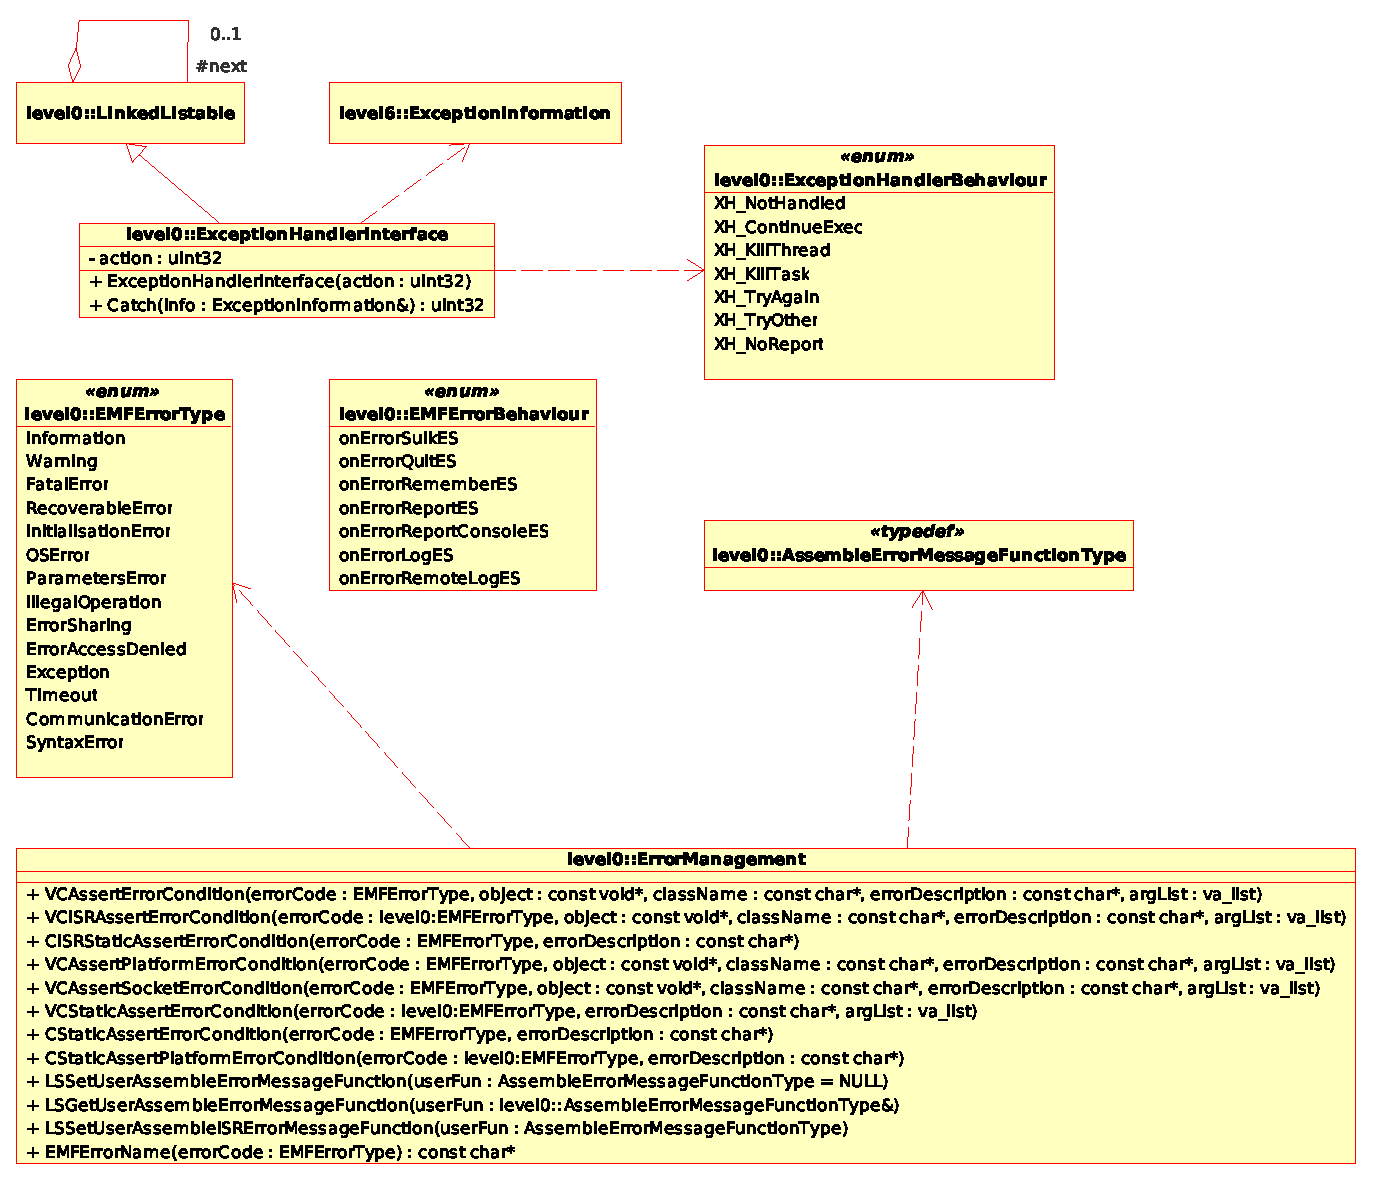
\includegraphics[width=0.93\textwidth]{level0/level0-err.eps}
  \caption{BaseLib Level0 errors and exceptions classes}
  \label{f:level0:err}
 \end{center}
\end{figure}

There are a great number of \texttt{enum}: \texttt{EMFErrorType} (in \textit{level0/ErrorManagement.h}), \texttt{EMFErrorBehaviour} (in \textit{level0/ErrorManagement.h})and \texttt{ExceptionHandlerBehaviour} (in \textit{level0/ExceptionHandlerDefinition.h}).



\subsubsection{ErrorManagement}
\texttt{[ErrorMamagemet.h, ErrorMamagemet.cpp]}\\
File \textit{level0/ErrorManagement.h} basically is a soup of C functions that print out formatted strings on some stream like for example the standard output or on a remote logger. Each function can be used in a precise scenario. Then follow a brief discussion about them.\\


Function \texttt{VCAssertErrorCondition} sets the error status and depending on setup does appropriate action; this call is to be called from static members. Function \texttt{VCISRAssertErrorCondition} like the previous one sets the error status and depending on setup does appropriate action, this call is to be called from Interrupt Service Routines. Function \texttt{CISRStaticAssertErrorCondition} sets the error status and depending on setup does appropriate action, also such call is to be called from Interrupt Service Routines (it is the same as the previous one except for the number of arguments, in such last function you have a variable argument list.\\ 

\texttt{VCAssertPlatformErrorCondition} sets the error status to \textit{platform error} and depending on setup does appropriate action, \texttt{VCAssertSocketErrorCondition} sets the error status to \textit{socket error} and depending on setup does appropriate action.\\

The function \texttt{VCStaticAssertErrorCondition} sets the error status and depending on setup does appropriate action, this call is to be called from static members; function \texttt{CStaticAssertErrorCondition} sets the error status and depending on setup does appropriate action, this call is to be called from static members. \texttt{CStaticAssertPlatformErrorCondition} sets the error status and depending on setup does appropriate action.

\begin{lstlisting}[
extendedchars=true,%
basicstyle=\fontfamily{pcr}\fontseries{m}\selectfont\footnotesize, %
stepnumber=1,%
numberstyle=\tiny,%
keywordstyle=\footnotesize\tt ,%
language=C++]
   void VCAssertErrorCondition(EMFErrorType errorCode,const void* object,
      const char* className,const char* errorDescription,va_list argList);
   void VCISRAssertErrorCondition(EMFErrorType errorCode,const void* object,
      const char* className,const char* errorDescription,va_list argList);
   void CISRStaticAssertErrorCondition(EMFErrorType errorCode,
      const char *errorDescription,...);

   void VCAssertPlatformErrorCondition(EMFErrorType errorCode,const void* object,
      const char* className,const char* errorDescription,va_list argList);
   void VCAssertSocketErrorCondition(EMFErrorType errorCode,const void* object,
      const char* className,const char* errorDescription,va_list argList);

   void VCStaticAssertErrorCondition(EMFErrorType errorCode,
      const char* errorDescription,va_list argList);
   void CStaticAssertErrorCondition(EMFErrorType errorCode,
      const char* errorDescription,...);
   void CStaticAssertPlatformErrorCondition(EMFErrorType errorCode,
      const char* errorDescription,...);
\end{lstlisting}

Function \texttt{LSSetUserAssembleErrorMessageFunction} sets the handler for error messages, function \texttt{LSGetUserAssembleErrorMessageFunction} gets a reference to the handler for error messages, \texttt{LSSetUserAssembleISRErrorMessageFunction} sets the handler for error messages coming from interrupts. Finally the function \texttt{EMFErrorName} translate an error encoded in \texttt{EMFErrorType} to an error name in C string format (\texttt{NULL}) terminated char array).

\begin{lstlisting}[
extendedchars=true,%
basicstyle=\fontfamily{pcr}\fontseries{m}\selectfont\footnotesize, %
stepnumber=1,%
numberstyle=\tiny,%
keywordstyle=\footnotesize\tt ,%
language=C++]
   void LSSetUserAssembleErrorMessageFunction(AssembleErrorMessageFunctionType userFun=NULL);
   void LSGetUserAssembleErrorMessageFunction(AssembleErrorMessageFunctionType &userFun);
   void LSSetUserAssembleISRErrorMessageFunction(AssembleErrorMessageFunctionType userFun);

   const char *EMFErrorName(EMFErrorType errorCode);
\end{lstlisting}



\subsubsection{ExceptionHandlerInterface}
\texttt{[ExceptionHandlerInterface.h]}\\
Class \texttt{ExceptionHandlerInterface} is an exception handler plugin interface. Is not a real C++ interface. There is only one abstract attribute \texttt{action} that defines what to do in case of exception. The constructor let you set the default handling in case of an exception. The method \texttt{Catch} return the action to be performed in case of an exception.

\begin{lstlisting}[
extendedchars=true,%
basicstyle=\fontfamily{pcr}\fontseries{m}\selectfont\footnotesize, %
stepnumber=1,%
numberstyle=\tiny,%
keywordstyle=\footnotesize\tt ,%
language=C++]
private:
   uint32 action;
public:
   ExceptionHandlerInterface(uint32 action=XH_NotHandled);
   virtual uint32 Catch(ExceptionInformation& info);
\end{lstlisting}



\subsection{Design Notes}
Take a look to Figure \ref{f:level0:err} is not a good design choice to have a dependency from level0 to level6: the code must be reorganized. The exception handling pluggable interface is a really nice idea.



\section{Memory}

This section group together classes depicted in Figure \ref{f:level0:mem}. Those classes have no strong link between them but are all about memory: shared memory handling, at OS level, is done by \texttt{SharedMemory} class, basic string management via \texttt{BString}; endianity support is handle via \texttt{Endianity} and memory basic type conversion is possible using \texttt{Intel16}, \texttt{IntelU16}, \texttt{Intel32},\texttt{IntelU32} classes. Such classes have to be extended also to \texttt{Intel64} and \texttt{IntelU64} as well.

\begin{figure}[h!]
 \begin{center}
  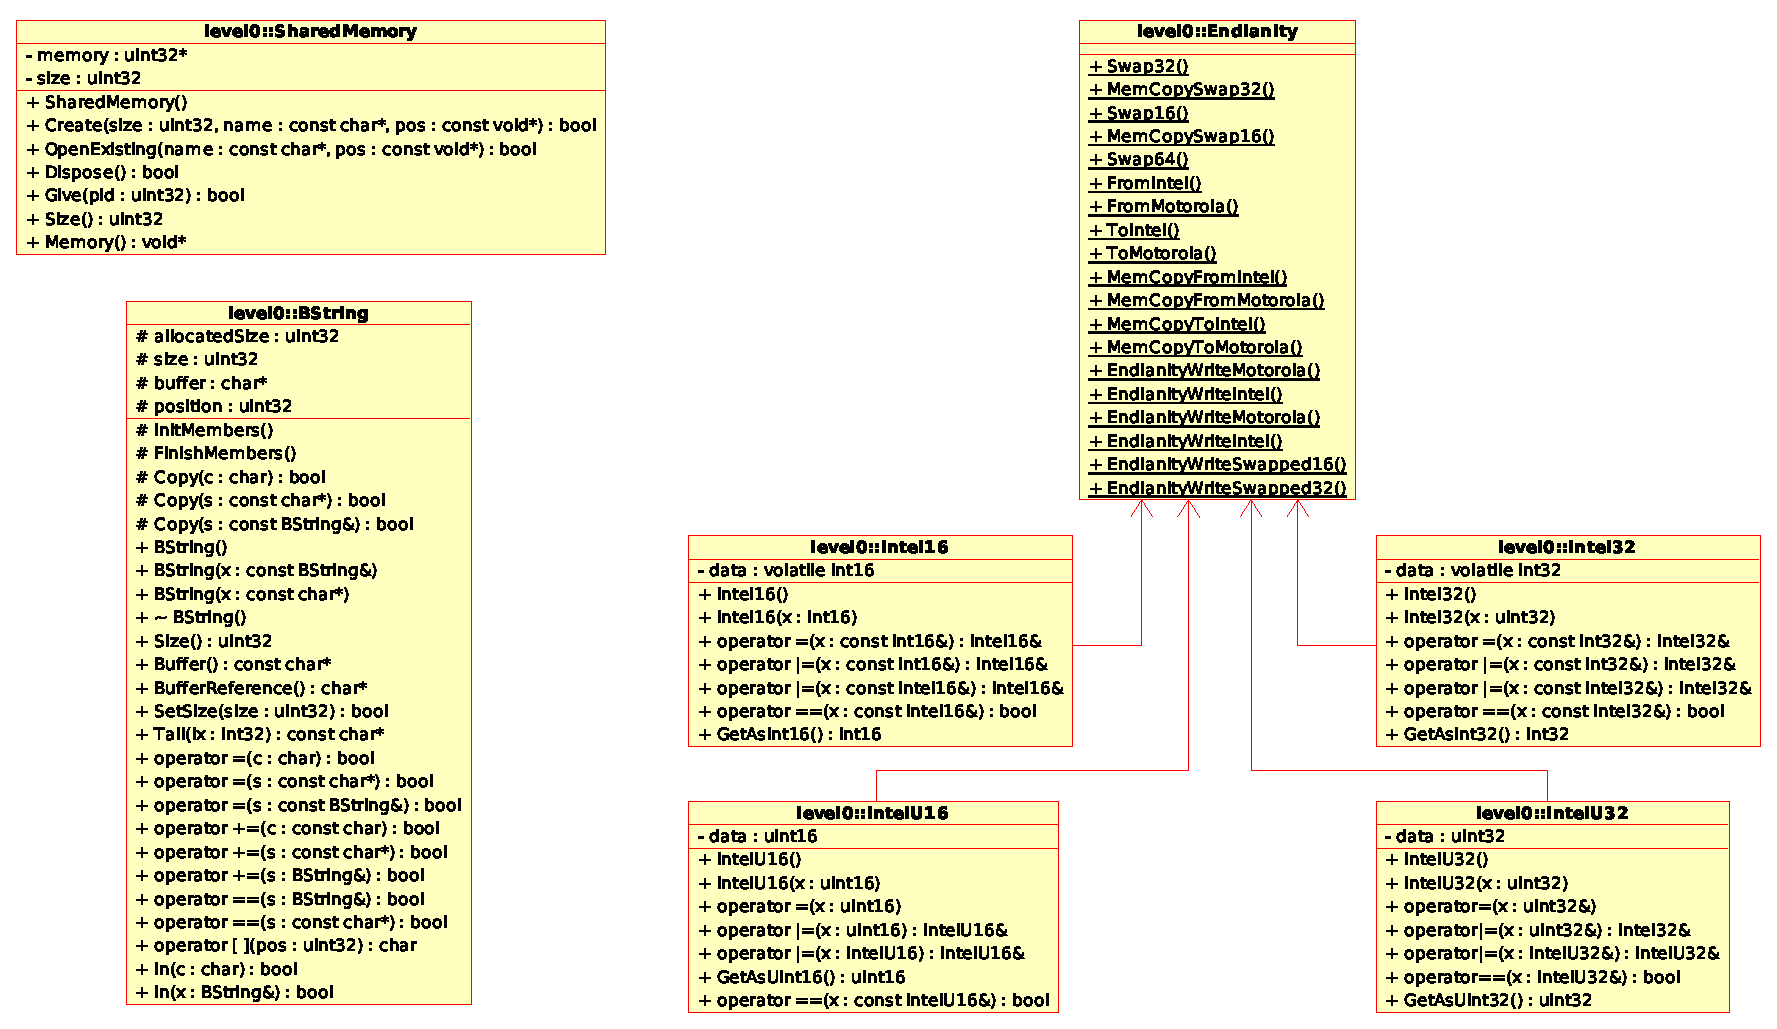
\includegraphics[width=\textwidth]{level0/level0-mem.eps}
  \caption{BaseLib Level0 memory classes}
  \label{f:level0:mem}
 \end{center}
\end{figure}

Some of those classes can be moved to a different category due to the implementation and logical dependency, for example class \texttt{SharedMemory} is thightly bounded to the OS so can be moved to \textit{arch} subdirectory, the same can be done for the class \texttt{Endianity} but that class has many dependecies in this section. Class \texttt{BString} can be moved to \textit{streams} subdirectory.



\subsubsection{SharedMemory}
\texttt{[SharedMemory.h, SharedMemory.cpp]}\\
This class is the most relevant in this group: it provides function to access shared memory. It holds attributes to the current shared memory address and to the current shared memory size (\texttt{memory}, \texttt{size}). There are others attributes with a strong dependence on the OS and OS's library, i.e. in Linux the class is implemented using SystemV Shared Memory.

\begin{lstlisting}[
extendedchars=true,%
basicstyle=\fontfamily{pcr}\fontseries{m}\selectfont\footnotesize, %
stepnumber=1,%
numberstyle=\tiny,%
keywordstyle=\footnotesize\tt ,%
language=C++]
private:
   uint32* memory;
   uint32 size;

#if (defined (_WIN32) || defined(_RSXNT))
   HANDLE handle;
#elif defined(_RTAI)
   unsigned long number;
#elif defined(_LINUX)
   key_t key;
   int id;
#endif
\end{lstlisting}

The constructor require no arguments and simply initialize the attributes in the class. \texttt{Size} simply return the size of the shared memory and \texttt{Memory} the start address of the shared memory, no check is done to test if the shared memory was just created or not, i.e. if the shared memory was not created jet the class must return an error.\\


The method \texttt{Create} create a new shared memory buffer by name \texttt{name} (in OS/2 the \texttt{pos} is disregarded); \texttt{OpenExisting} is used to open an existing share memory in the system by name.
Last two functions are from OS/2 operating system and are not fully ported to other operating systems. \texttt{Dispose} dispose the use of the shared memory and \texttt{Give} release the use of the shared memory. If \texttt{Create} is used to create a shared memory then \texttt{Dispose} is used to return the shared memory to the system. Pay attention that no destructor is coded so is not safe to not return the memory to the system. Difference between \texttt{Give} and \texttt{Dispose} is not really clear.

\begin{lstlisting}[
extendedchars=true,%
basicstyle=\fontfamily{pcr}\fontseries{m}\selectfont\footnotesize, %
stepnumber=1,%
numberstyle=\tiny,%
keywordstyle=\footnotesize\tt ,%
language=C++]
public:
   SharedMemory();
   uint32 Size();
   void* Memory();

   bool Create(uint32 size,const char* name,const void* pos=0);
   bool OpenExisting(const char* name,const void* pos=0);
   bool Dispose(void)
   bool Give(uint32 pid);
\end{lstlisting}



\subsubsection{BString}
\texttt{[BString.h, BString.cpp]}\\
The class \texttt{BString} is the basic implementation of a string, the class want let user treat a string like a file; reading and writing are done on a specific position.\\


Starting with the attributes, the first attribute, \texttt{allocatedSize}, is the size of the allocated memory block for the string; \texttt{size} represent the size of the used memory block minus one (it excludes the 0 char); \texttt{buffer} holds the memory buffer address and \texttt{position} is the currently seek position.\\


Other protected methods are: \texttt{InitMembers} and \texttt{FinishMembers} used for constructor and deconstructor.
Copy methods (\texttt{Copy}) let the user copy a character, a string and a \texttt{BString} into the \texttt{BString} buffer.

\begin{lstlisting}[
extendedchars=true,%
basicstyle=\fontfamily{pcr}\fontseries{m}\selectfont\footnotesize, %
stepnumber=1,%
numberstyle=\tiny,%
keywordstyle=\footnotesize\tt ,%
language=C++]
protected:
   uint32 allocatedSize;
   uint32 size;
   char* buffer;
   uint32 position;

   void InitMembers();
   void FinishMembers();

   bool Copy(char* c);
   bool Copy(const char* s);
   bool Copy(const BString& s);
\end{lstlisting}

The first constructor creates an empty string; second constructor is the copy constructor and the last constructor build up a \texttt{BString} starting from a C string. Then cames the destructor.

The method \texttt{Size} return the size of the string (\texttt{size} attribute); \texttt{SetSize} clips the string size to a specified point (\texttt{size} is expressed from the start of the string). \texttt{Buffer} returns a read only access to the internal buffer, \texttt{BufferReference} returns a read/write access to the internal buffer and \texttt{Tail} returns a read only pointer to the tail of the buffer.

Methods \texttt{In} checks if a char is in the string.

\begin{lstlisting}[
extendedchars=true,%
basicstyle=\fontfamily{pcr}\fontseries{m}\selectfont\footnotesize, %
stepnumber=1,%
numberstyle=\tiny,%
keywordstyle=\footnotesize\tt ,%
language=C++]
public:
   inline BString();
   inline BString(const BString& x);
   inline BString(const char* x);
   virtual ~BString();

   inline uint32 Size() const;
   inline bool SetSize(uint32 size);

   inline const char* Buffer() const;
   inline char* BufferReference() const;
   inline const char* Tail(int32 ix ) const;

   inline bool In(char c) const;
   inline bool In(BString& x) const;
\end{lstlisting}

The following operators redefinition eases the work with strings. First three \texttt{operator=} lets sets a \texttt{BString} to be a copy of the input parameter; methods \texttt{operator+=} address the concatenation between a \texttt{BString} and a single char, a C string and a \texttt{BString} object; redefinition of \texttt{opertator==} lets compare differents string objects. \texttt{operator[]} allows access to character within the buffer, argument \texttt{pos} is the position in the buffer to be accessed.

\begin{lstlisting}[
extendedchars=true,%
basicstyle=\fontfamily{pcr}\fontseries{m}\selectfont\footnotesize, %
stepnumber=1,%
numberstyle=\tiny,%
keywordstyle=\footnotesize\tt ,%
language=C++]
   inline bool operator=(char c);
   inline bool operator=(const char *s);
   inline bool operator=(const BString &s);
   inline bool operator+=(const char c);
   inline bool operator+=(const char *s);
   inline bool operator+=(BString &s);
   inline bool operator==(BString &s) const;
   inline bool operator==(const char *s) const;
   inline char operator[](uint32 pos);
\end{lstlisting}



\subsubsection{Endianity}
\texttt{[Endianity.h]}\\
The endianity class implements endianity conversion between types. Basically many methods were cut in Figure \ref{f:level0:mem} to fit the UML schema in the page. We now explore the methods it offers.

Core methods are first coded and basically do all the work. The first \texttt{Swap32} method swaps the 4 bytes in a 32 bit number, i.e. simply changes the endianity; the second \texttt{Swap32} swaps 4 bytes in a 32bit vector; \texttt{MemCopySwap32} swaps the 4 bytes while copying a vector of 32 bit numbers.

The first \texttt{Swap16} method swaps the 2 bytes in a 16 bit number, i.e. changes the endianity; the second \texttt{Swap16} swaps 2 bytes in a 16bit vector; \texttt{MemCopySwap16} swaps the 2 bytes while copying a vector of 16 bit numbers.

Last \texttt{Swap64} method swaps the 8 bytes in a 64 bit number.

\begin{lstlisting}[
extendedchars=true,%
basicstyle=\fontfamily{pcr}\fontseries{m}\selectfont\footnotesize, %
stepnumber=1,%
numberstyle=\tiny,%
keywordstyle=\footnotesize\tt ,%
language=C++]
public:
   static inline void Swap32(volatile void *x);
   static inline void Swap32(volatile void *x,uint32 sizer);
   static inline void MemCopySwap32(volatile void *dest,volatile const void *src,uint32 sizer);

   static inline void Swap16(volatile void *x);
   static inline void Swap16(volatile void *x,uint32 sizer);
   static inline void MemCopySwap16(volatile void *dest,volatile const void *src,uint32 sizer);

   static inline void Swap64(volatile void *x);
\end{lstlisting}

The following function has a different implementation if compiled on different architecture (infact this class will be moved in \textit{arch}). The first overloaded method \texttt{FromMotorola} need in input a number in \textit{Motorola} format (i.e. big endian) and convert it in the currently system endianity format. \texttt{FromIntel} need in input a number in \textit{Intel} format (i.e. little endian) and convert it in the currently system endianity format. \texttt{ToMotorola} covert the value in big endian and \texttt{ToIntel} convert the value in little endian.

All such methods use the before presented methods.

\begin{lstlisting}[
extendedchars=true,%
basicstyle=\fontfamily{pcr}\fontseries{m}\selectfont\footnotesize, %
stepnumber=1,%
numberstyle=\tiny,%
keywordstyle=\footnotesize\tt ,%
language=C++]
   static inline void FromMotorola(volatile double &x);
   static inline void FromMotorola(volatile float &x);
   static inline void FromMotorola(volatile uint64 &x);
   static inline void FromMotorola(volatile uint32 &x);
   static inline void FromMotorola(volatile uint16 &x);
   static inline void FromMotorola(volatile int64 &x);
   static inline void FromMotorola(volatile int32 &x);
   static inline void FromMotorola(volatile int16 &x);

   static inline void FromIntel(volatile double &x);
   static inline void FromIntel(volatile float &x);
   static inline void FromIntel(volatile uint64 &x);
   static inline void FromIntel(volatile uint32 &x);
   static inline void FromIntel(volatile uint16 &x);
   static inline void FromIntel(volatile int64 &x);
   static inline void FromIntel(volatile int32 &x);
   static inline void FromIntel(volatile int16 &x);

   static inline void ToMotorola(volatile double &x);
   static inline void ToMotorola(volatile float &x);
   static inline void ToMotorola(volatile uint64 &x);
   static inline void ToMotorola(volatile uint32 &x);
   static inline void ToMotorola(volatile uint16 &x);
   static inline void ToMotorola(volatile int64 &x);
   static inline void ToMotorola(volatile int32 &x);
   static inline void ToMotorola(volatile int16 &x);

   static inline void ToIntel(volatile double &x);
   static inline void ToIntel(volatile float &x);
   static inline void ToIntel(volatile uint64 &x);
   static inline void ToIntel(volatile uint32 &x);
   static inline void ToIntel(volatile uint16 &x);
   static inline void ToIntel(volatile int64 &x);
   static inline void ToIntel(volatile int32 &x);
   static inline void ToIntel(volatile int16 &x);
\end{lstlisting}

The group of methods that comes are really equivalent to the ones above but instead of swapping a single value they swap an entire vector of values. The signature of methods is fully reported here.

\begin{lstlisting}[
extendedchars=true,%
basicstyle=\fontfamily{pcr}\fontseries{m}\selectfont\footnotesize, %
stepnumber=1,%
numberstyle=\tiny,%
keywordstyle=\footnotesize\tt ,%
language=C++]
   static inline void MemCopyFromMotorola(float *dest,const float *src,uint32 size);
   static inline void MemCopyFromMotorola(uint32 *dest,const uint32 *src,uint32 size);
   static inline void MemCopyFromMotorola(uint16 *dest,const uint16 *src,uint32 size);
   static inline void MemCopyFromMotorola(int32 *dest,const int32 *src,uint32 size);
   static inline void MemCopyFromMotorola(int16 *dest,const int16 *src,uint32 size);

   static inline void MemCopyFromIntel(float *dest,const float *src,uint32 size);
   static inline void MemCopyFromIntel(uint32 *dest,const uint32 *src,uint32 size);
   static inline void MemCopyFromIntel(uint16 *dest,const uint16 *src,uint32 size);
   static inline void MemCopyFromIntel(int32 *dest,const int32 *src,uint32 size);
   static inline void MemCopyFromIntel(int16 *dest,const int16 *src,uint32 size);

   static inline void MemCopyToMotorola(float *dest,const float *src,uint32 size);
   static inline void MemCopyToMotorola(uint32 *dest,const uint32 *src,uint32 size);
   static inline void MemCopyToMotorola(uint16 *dest,const uint16 *src,uint32 size);
   static inline void MemCopyToMotorola(int32 *dest,const int32 *src,uint32 size);
   static inline void MemCopyToMotorola(int16 *dest,const int16 *src,uint32 size);

   static inline void MemCopyToIntel(float *dest,const float *src,uint32 size);
   static inline void MemCopyToIntel(uint32 *dest,const uint32 *src,uint32 size);
   static inline void MemCopyToIntel(uint16 *dest,const uint16 *src,uint32 size);
   static inline void MemCopyToIntel(int32 *dest,const int32 *src,uint32 size);
   static inline void MemCopyToIntel(int16 *dest,const int16 *src,uint32 size);
\end{lstlisting}

Last methods, that are to be moved to streams, all use the \texttt{fwrite} function (binary stream output) but does the same things as the one above.

\begin{lstlisting}[
extendedchars=true,%
basicstyle=\fontfamily{pcr}\fontseries{m}\selectfont\footnotesize, %
stepnumber=1,%
numberstyle=\tiny,%
keywordstyle=\footnotesize\tt ,%
language=C++]
   static inline void EndianityWriteMotorola(int8 &x,FILE *f);
   static inline void EndianityWriteMotorola(int16 &x,FILE *f);
   static inline void EndianityWriteMotorola(int32 &x,FILE *f);
   static inline void EndianityWriteMotorola(uint8 &x,FILE *f);
   static inline void EndianityWriteMotorola(uint16 &x,FILE *f);
   static inline void EndianityWriteMotorola(uint32 &x,FILE *f);

   static inline void EndianityWriteIntel(int8 &x,FILE *f);
   static inline void EndianityWriteIntel(int16 &x,FILE *f);
   static inline void EndianityWriteIntel(int32 &x,FILE *f);
   static inline void EndianityWriteIntel(uint8 &x,FILE *f);
   static inline void EndianityWriteIntel(uint16 &x,FILE *f);
   static inline void EndianityWriteIntel(uint32 &x,FILE *f);

   static inline void EndianityWriteMotorola(int8 *x,uint32 n,FILE *f);
   static inline void EndianityWriteMotorola(int16 *x,uint32 n,FILE *f);
   static inline void EndianityWriteMotorola(int32 *x,uint32 n,FILE *f);
   static inline void EndianityWriteMotorola(uint8 *x,uint32 n,FILE *f);
   static inline void EndianityWriteMotorola(uint16 *x,uint32 n,FILE *f);
   static inline void EndianityWriteMotorola(uint32 *x,uint32 n,FILE *f);

   static inline void EndianityWriteIntel(int8 *x,uint32 n,FILE *f);
   static inline void EndianityWriteIntel(int16 *x,uint32 n,FILE *f);
   static inline void EndianityWriteIntel(int32 *x,uint32 n,FILE *f);
   static inline void EndianityWriteIntel(uint8 *x,uint32 n,FILE *f);
   static inline void EndianityWriteIntel(uint16 *x,uint32 n,FILE *f);
   static inline void EndianityWriteIntel(uint32 *x,uint32 n,FILE *f);

   static void EndianityWriteSwapped16(void *x,uint32 n,FILE *f);
   static void EndianityWriteSwapped32(void *x,uint32 n,FILE *f);
\end{lstlisting}



\subsubsection{Intel16, IntelU16, Intel32, IntelU32}
\texttt{[Intel16.h, IntelU16.h, Intel32.h, IntelU32.h]}\\
Those classes implements a 16 bit integer in little endian encoding, a 16 bit unsigned int in little endian encoding, a 32 bit integer in little endian encoding and a 32 bit unsigned integer in little endian encoding.

Basically they all have the same interface with the same methods, constructors and operators ridefinition. We just cut and past the class definition of \texttt{Intel16}.

\begin{lstlisting}[
extendedchars=true,%
basicstyle=\fontfamily{pcr}\fontseries{m}\selectfont\footnotesize, %
stepnumber=1,%
numberstyle=\tiny,%
keywordstyle=\footnotesize\tt ,%
language=C++]
class Intel16 {
private:
   volatile int16 data;
public:
   inline Intel16();
   inline Intel16(int16 x);

   inline Intel16& operator= (const int16& x);
   inline Intel16& operator|= (const int16& x);
   inline Intel16& operator|= (const Intel16& x);
   inline bool operator == (const Intel16& x);

   inline int16 GetAsInt16();
};
\end{lstlisting}



\subsection{Design Notes}
This section doesn't need to much notes because classes are probably not well grouped together. Some class can be moved to another groups.
It is really important that the \texttt{SharedMemory} class has a distructor that will destroy the give back the shared memory helded to keep resource consumption under control.



\section{Processes, Threads}

\begin{figure}[h!]
 \begin{center}
  \includegraphics[width=\textwidth]{level0/level0-proc.eps}
  \caption{BaseLib Level0 proc classes}
  \label{f:level0:proc}
 \end{center}
\end{figure}

\subsubsection{ThreadInitialisationInterface}
\texttt{[ThreadInitialisationInterface.h]}\\
This class stores information associated with a specific thread. Such class is an interface used to implement a common thread initialisation procedure; despite the name \texttt{ThreadInitialisationInterface} it also provides a minimal set of functionalities; for this reason it has not been made pure virtual and can be istantiated. Let's take a look at its attributes and methods.\\

The type of a function that can be used for a thread is typedefined in \textit{level0/ThreadInitialistionInterface.h}
\begin{lstlisting}[
extendedchars=true,%
basicstyle=\fontfamily{pcr}\fontseries{m}\selectfont\footnotesize, %
stepnumber=1,%
numberstyle=\tiny,%
keywordstyle=\footnotesize\tt ,%
language=C++]
typedef void (*ThreadFunctionType)(void *parameters);
\end{lstlisting}
The attribute \texttt{userThreadFunction} is of type \texttt{ThreadFunctionType} and is the holder of a thread entry point. \texttt{userData} is
 a pointer to a structure containing thread data and \textit{name} is the name of the thread. Last attribute, a \texttt{public} one holds the thread number.

\begin{lstlisting}[
extendedchars=true,%
basicstyle=\fontfamily{pcr}\fontseries{m}\selectfont\footnotesize, %
stepnumber=1,%
numberstyle=\tiny,%
keywordstyle=\footnotesize\tt ,%
language=C++]
protected:
   ThreadFunctionType userThreadFunction;
   void* userData;
   const char* name;
public:
   TID tid;
\end{lstlisting}

There is an \texttt{operation=} ridefinition and a copy constructor; other two constructors create a new \texttt{NULL} object and a new object with a new \texttt{ThreadFunctionType}, a \texttt{userData} and a \texttt{name}.

The method \texttt{UserThreadFunction} execute the registered thread; \texttt{GetThreadName} gets the name of the thread and \texttt{ExceptionProtectedExecute} allows to call a subroutine within an exception handler protection, this implementation is a dummy one, so it must be recoded at higher levels (i.e. to be subclassed).

\begin{lstlisting}[
extendedchars=true,%
basicstyle=\fontfamily{pcr}\fontseries{m}\selectfont\footnotesize, %
stepnumber=1,%
numberstyle=\tiny,%
keywordstyle=\footnotesize\tt ,%
language=C++]
   void operator=(ThreadInitialisationInterface &tii);
   ThreadInitialisationInterface(ThreadInitialisationInterface& tii);

   ThreadInitialisationInterface();
   ThreadInitialisationInterface(ThreadFunctionType userThreadFunction,
      void* userData, const char* name);
   virtual ~ThreadInitialisationInterface();

   virtual void UserThreadFunction();
   virtual const char *GetThreadName();
   bool ExceptionProtectedExecute(ThreadFunctionType userFunction,
      void *userData, ExceptionHandlerInterface *eh);
\end{lstlisting}



\subsubsection{Threads DataBase}
\texttt{[ThreadsDatabase.h,ThreadsDatabase.cpp]}\\
The \textit{Threads DataBase} is not a class but a set of function. It is depicted in Figure \ref{f:level0:proc} only for dependency purpouse. Such entity is a register of all the threads currently running (or expected to be running) in the system. All functions that lets you manage the \textit{Threads DataBase} follows, functions can be founded in \textit{level0/ThreadsDatabase.h}.\\


\textit{Threads DataBase} (TDB) is managed via the class \texttt{Threads} the following three functions are only accessible by \textit{level0/Threads.cpp} (i.e. are not exported or declared anywhere else).
The method \texttt{TDB\_NewEntry} creates new TDB entry associated to the \texttt{ThreadInitialisationInterface} object passed by pointer. Note that a \texttt{Threads} object is not a subclass of \texttt{ThreadInitialisationInterface}. The method \texttt{TDB\_RemoveEntry} destroy the TDB entry associated wtih the current calling thread, note that the method has no arguments. The method \texttt{TDB\_GetTII} access private thread information, on timeout returns \texttt{NULL}.

\begin{lstlisting}[
extendedchars=true,%
basicstyle=\fontfamily{pcr}\fontseries{m}\selectfont\footnotesize, %
stepnumber=1,%
numberstyle=\tiny,%
keywordstyle=\footnotesize\tt ,%
language=C++]
   bool TDB_NewEntry(ThreadInitialisationInterface *tii);
   ThreadInitialisationInterface* TDB_RemoveEntry();
   ThreadInitialisationInterface* TDB_GetTII(TID tid=0);
\end{lstlisting}

Now comes some generic usable functions. Every time a user want to access the TDB it must request a lock to use it with \texttt{TDB\_Lock} and unlock with \texttt{TDB\_UnLock}.

The method \texttt{TDB\_NumberOfThreads} returns the number of threads registered in the database. \texttt{TDB\_GetThreadID} retrieves the TID of thread \texttt{n}, the method \texttt{TDB\_Find} return the TID of thread named \texttt{name}.
\texttt{TDB\_GetInfo} retrieves information about a thread identified either by \texttt{name} or \texttt{TID} or index; \texttt{TDB\_GetName} retrieves pointer to name in \texttt{ThreadInitialisationInterface} attribute for current thread.

\begin{lstlisting}[
extendedchars=true,%
basicstyle=\fontfamily{pcr}\fontseries{m}\selectfont\footnotesize, %
stepnumber=1,%
numberstyle=\tiny,%
keywordstyle=\footnotesize\tt ,%
language=C++]
   bool TDB_Lock(TimeoutType tt = TTInfiniteWait);
   bool TDB_UnLock();

   int TDB_NumberOfThreads();
   TID TDB_GetThreadID(int n);
   TID TDB_Find(const char* name);
   bool TDB_GetInfo(ThreadInitialisationInterface& tiiCopy,
      int n=-1,const char* name=NULL,TID tid=(TID)-1);
   const char* TDB_GetName();
\end{lstlisting}

Differently with others \textit{DataBase}'s structures this \textit{Threads DataBase} doesn't relay on a linked list but on an array of pointers to \texttt{ThreadInitialisationInterface} objects.



\subsubsection{Threads}
\texttt{[Threads.h, Threads.cpp]}\\

This is the core threads class, it provides for thread registration in the \textit{Threads Database} and provide a complete interface to thread managment (processors mask are managed via the \texttt{ProcessorType} class).\\


The method \texttt{SetThreadInitialisationInterfaceConstructor} sets the function used to build the thread initialisation interface. An \texttt{ThreadInitialisationInterface} object is created using either the default value or the parameter passed to the function by the \texttt{BeginThread} method. The method \texttt{SetPriorityLevel} changes thread priority; applies only to current thread 0..31 (on windows it is actually /4 ). \texttt{EndThread} is called implicitly at the end of the main thread function, calling this method leaves some allocated memory unfreed. Calling \texttt{BeginThread} will start a thred this method will dynamically allocate an object of type \texttt{ThreadInitialisationInterface} using the function hook \texttt{ThreadInitialisationInterfaceConstructor}; this allows the programmer to choose which constructor has to be used in the case a \texttt{ThreadInitialisationInterface} derived class had been used.

In BaseLib that is a thread based library there are four classes of priority (from the maximum priority to the minimum priority):
\begin{itemize}
 \item RealTime
 \item High
 \item Normal
 \item Low
\end{itemize}

\texttt{Threads} class define only static methods so each static method apply to the current executed thread. You can change the thread priority using \texttt{SetRealTimeClass}, \texttt{SetHighClass}, \texttt{SetNormalClass} and \texttt{SetLowClass}.

\texttt{ThreadId} method gets the current thread id; \texttt{Kill} kills a thread asynchronously; \texttt{IsAlive} checks whether thread \texttt{tid} is still alive. The method \texttt{GetName} basically retrieve thread's name.

\begin{lstlisting}[
extendedchars=true,%
basicstyle=\fontfamily{pcr}\fontseries{m}\selectfont\footnotesize, %
stepnumber=1,%
numberstyle=\tiny,%
keywordstyle=\footnotesize\tt ,%
language=C++]
public:
   static void SetThreadInitialisationInterfaceConstructor(ThreadInitialisationInterfaceConstructorType tiic);
   static void SetPriorityLevel(uint32 level);

   static void EndThread();
   static TID BeginThread(ThreadFunctionType function,
      void* parameters = NULL,
      uint32 stacksize=THREADS_DEFAULT_STACKSIZE,
      const char* name=NULL,
      ExceptionHandlerBehaviour exceptionHandlerBehaviour=XH_NotHandled,
      ProcessorType runOnCPUs=PTDefaultCPUs);

   static void SetNormalClass();
   static void SetRealTimeClass();
   static void SetIdleClass();
   static void SetHighClass();

   static TID ThreadId();
   static bool Kill(TID tid);
   static bool IsAlive(TID tid);
   static const char *GetName();
\end{lstlisting}



\subsubsection{Processes}
\texttt{[Processes.h]}\\
The class \texttt{Processes} give an interface to operating system wide functions like creating a process, i.e. loading an executable file, process index, killing a process and reboot the system. The description of functions interface follows.\\

The method \texttt{GetThisPid} returns the current's process id and \texttt{ProcessName} retrieves the name of this applicationm, it is obtained by parsing \texttt{argv[0]} it does not work if \texttt{REAL\_MAIN} is defined.\\

Methods \texttt{Detach} and \texttt{Start} are exactly the same method for every system except OS/2. \texttt{Detach} method launchs a specified command as a newly detached process and return the task id of the new process or 0 if the process has not been created; \texttt{command} argument is a pointer to a string containing the command to execute (i.e. the application that will run); \texttt{args} argument is a pointer to a string containing the arguments of the command; \texttt{path} is a pointer to a string containing the path to the command. \\

The method \texttt{Kill} lets the user kill the process specified by the \texttt{task\_id}; \texttt{IsAlive} lets query the system to know if the process specified by argument is alive; last method: \texttt{Reboot} causes the machine to reboot.

\begin{lstlisting}[
extendedchars=true,%
basicstyle=\fontfamily{pcr}\fontseries{m}\selectfont\footnotesize, %
stepnumber=1,%
numberstyle=\tiny,%
keywordstyle=\footnotesize\tt ,%
language=C++]
public:
   static uint32 GetThisPid();
   static const char *ProcessName();
   
   static uint32 Detach(const char *command,const char *args,const char *path = NULL);
   static uint32 Start(const char *command,const char *args,const char *path=NULL);
   static bool Kill(uint32 task_id);
   static bool IsAlive(uint32 task_id);

   static void Reboot();
\end{lstlisting}



\subsection{Design Notes}

Class \texttt{Processes} is likely to be moved in directory \textit{arch}. I'm not sure about the need of a \texttt{ThreadInitializationInterface}, a \texttt{ThreadInterface} can be better.



\section{Mathematic}
In this section there are some class involving mathematical conversion and complex number handling. Classes in this seciton are here listed and depicted in Figure \ref{f:level0:math}.
\begin{itemize}
 \item Complex
 \item NordFloat
 \item FastMath
\end{itemize}

\begin{figure}[h!]
 \begin{center}
  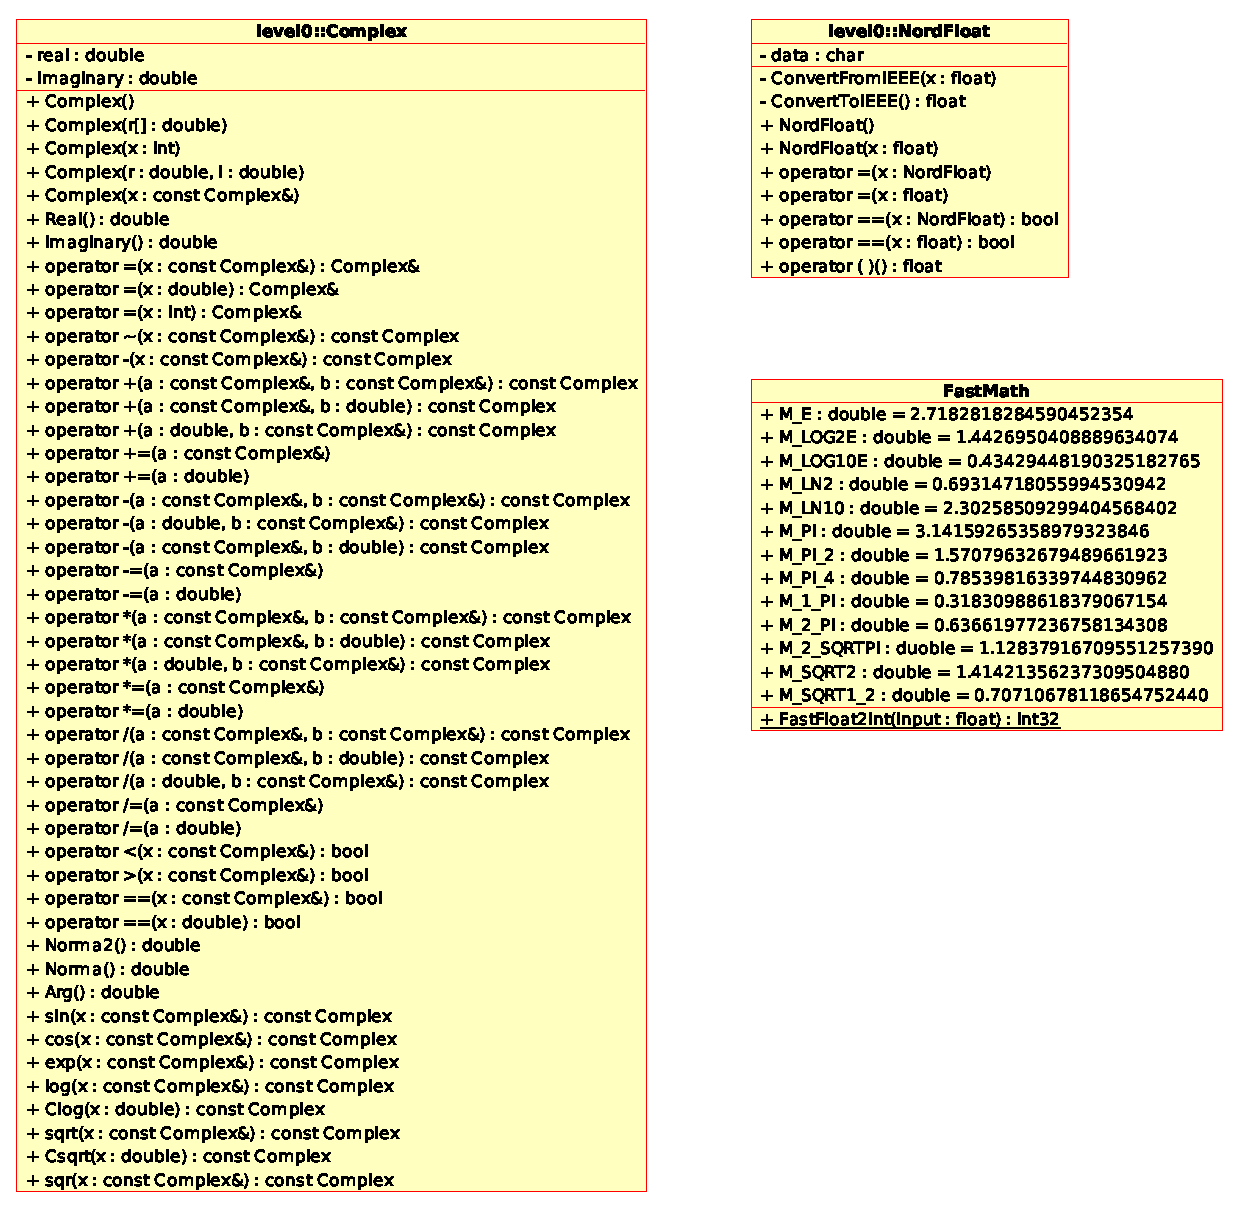
\includegraphics[width=0.73\textwidth]{level0/level0-math.eps}
  \caption{BaseLib Level0 math classes}
  \label{f:level0:math}
 \end{center}
\end{figure}



\subsubsection{Complex}
\texttt{Complex.h}\\

Comples is an implementation of the complex numerical type as 2 doubles.

The structure of the class is straightforward: it relies on two \texttt{double} attributes: \texttt{real} that holds the real part of the complex number and \texttt{imaginary} that holds the imaginary part of the complex number. There are some contructors; the first one takes no arguments, the second and third take only one argument:the real part (\texttt{double} and \texttt{int}), fourth and fifth take two doubles as the real and imaginary parts, last constructor is the copy constructor. 

There are two set methods \texttt{Real} that return the real part of the number and \texttt{Complex} that return the complex part.

\begin{lstlisting}[
extendedchars=true,%
basicstyle=\fontfamily{pcr}\fontseries{m}\selectfont\footnotesize, %
stepnumber=1,%
numberstyle=\tiny,%
keywordstyle=\footnotesize\tt ,%
language=C++]
private:
   double real;
   double imaginary;
public:
   inline Complex();
   inline Complex(double x);
   inline Complex(int x);
   inline Complex(double r,double i);
   inline Complex(double r[2]);

   inline Complex (const Complex &x);

   inline double Real();
   inline double Imaginary();
\end{lstlisting}

The class redefine all the mathematical operators using complex numbers. \texttt{operator~} return the complex conjugate of the number.

\begin{lstlisting}[
extendedchars=true,%
basicstyle=\fontfamily{pcr}\fontseries{m}\selectfont\footnotesize, %
stepnumber=1,%
numberstyle=\tiny,%
keywordstyle=\footnotesize\tt ,%
language=C++]
   inline Complex& operator=(const Complex &x);
   inline Complex& operator=(double x);
   inline Complex& operator=(int x);

   inline friend const Complex operator~(const Complex &x);
   inline friend const Complex operator-(const Complex &x);
   inline friend const Complex operator+(const Complex &a,const Complex &b);

   inline friend const Complex operator+(const Complex &a,double b);
   inline friend const Complex operator+(double a,const Complex &b);

   inline void operator+=(const Complex &a);
   inline void operator+=(double a);

   inline friend const Complex operator-(const Complex &a,const Complex &b);
   inline friend const Complex operator-(double a,const Complex &b);
   inline friend const Complex operator-(const Complex &a,double b);

   inline void operator-=(const Complex &a);
   inline void operator-=(double a);

   inline friend const Complex operator*(const Complex &a,const Complex &b)
   inline friend const Complex operator*(const Complex &a,double b);
   inline friend const Complex operator*(double a,const Complex &b);

   inline void operator*=(const Complex &a);
   inline void operator*=(double a);

   inline friend const Complex operator/(const Complex &a,const Complex &b);
   inline friend const Complex operator/(const Complex &a,double b);
   inline friend const Complex operator/(double a,const Complex &b);

   inline void operator/=(const Complex &a);
   inline void operator/=(double a);
   inline bool operator< (const Complex &x);
   inline bool operator> (const Complex &x);
   inline bool operator== (const Complex &x);
   inline bool operator== (double x);
\end{lstlisting}

There are also a set of simple mathematical functions. \texttt{Norma2} returns the norma squared, \texttt{Norma} return the norma and \texttt{Arg} return the argument (?).

\begin{lstlisting}[
extendedchars=true,%
basicstyle=\fontfamily{pcr}\fontseries{m}\selectfont\footnotesize, %
stepnumber=1,%
numberstyle=\tiny,%
keywordstyle=\footnotesize\tt ,%
language=C++]
   inline friend const Complex sin(const Complex &x);
   inline friend const Complex cos(const Complex &x);
   inline friend const Complex exp(const Complex &x);
   inline friend const Complex log(const Complex &x);
   inline friend const Complex Clog(double x);
   inline friend const Complex sqrt(const Complex &x);
   inline friend const Complex Csqrt(double x);
   inline friend const Complex sqr(const Complex &x);

   inline double Norma2()const;
   inline double Norma()const;
   inline double Arg()const;
\end{lstlisting}



\subsubsection{NordFloat}
\texttt{NordFloat.h}\\
Class \texttt{NordFloat} converts a float between network byte order (\textit{Nord}) and Intel byte order. There is only one attribute: \texttt{data} that is a \texttt{char[6]} array; there are two private methods that address the conversion between formats. There are constructors one zero constructor and one constructor that takes a \texttt{float}. Some operators are also defined.

\begin{lstlisting}[
extendedchars=true,%
basicstyle=\fontfamily{pcr}\fontseries{m}\selectfont\footnotesize, %
stepnumber=1,%
numberstyle=\tiny,%
keywordstyle=\footnotesize\tt ,%
language=C++]
private:
   char data[6];

   void ConvertFromIEEE(float x);
   float ConvertToIEEE();
public:
    NordFloat();
    NordFloat(float x);

    void operator=(NordFloat x);
    void operator=(float x);
    bool operator==(NordFloat x);
    bool operator==(float x);
    float operator()();
\end{lstlisting}



\subsubsection{FastMath}
\texttt{FastMath.h}\\
Source \textit{FastMath.h} doesn't define a class but for illustrative needes it is represented like a class in Figure \ref{f:level0:math}. The file contains one function definition and many mathematical constants. Function \texttt{FastFloat2Int} converts a float to an integer using processor instructions (will be moved in \textit{arch/}.

\begin{lstlisting}[
extendedchars=true,%
basicstyle=\fontfamily{pcr}\fontseries{m}\selectfont\footnotesize, %
stepnumber=1,%
numberstyle=\tiny,%
keywordstyle=\footnotesize\tt ,%
language=C++]
static inline int32 FastFloat2Int(float input);
\end{lstlisting}

Constants follow in Table \ref{t:math:constants}

\begin{table}[!h]
 \begin{center}
  \begin{tabular}{lll}
    $e$ & \texttt{M\_E} & 2.7182818284590452354 \\
    $log2(e)$ & \texttt{M\_LOG2E} & 1.4426950408889634074 \\
    $log10(e)$ & \texttt{M\_LOG10E} & 0.43429448190325182765 \\
    $log(2)$ & \texttt{M\_LN2} & 0.69314718055994530942 \\
    $log(10)$ & \texttt{M\_LN10} & 2.30258509299404568402 \\
    $pi$ & \texttt{M\_PI} & 3.14159265358979323846 \\
    $pi/2$ & \texttt{M\_PI\_2} & 1.57079632679489661923 \\
    $pi/4$ & \texttt{M\_PI\_4} & 0.78539816339744830962 \\
    $1/pi$ & \texttt{M\_1\_PI} & 0.31830988618379067154 \\
    $2/pi$ & \texttt{M\_2\_PI} & 0.63661977236758134308 \\
    $2/sqrt(pi)$ & \texttt{M\_2\_SQRTPI} & 1.12837916709551257390 \\
    $sqrt(2)$ & \texttt{M\_SQRT2} & 1.41421356237309504880 \\
    $sqrt(1/2)$ & \texttt{M\_SQRT1\_2} & 0.70710678118654752440 \\
   \end{tabular}
   \end{center}
  \caption{constants in \texttt{FastMath}}
 \label{t:math:constants}
\end{table}



\subsection{Design Notes}
The aim of class \texttt{NordFloat} is not really clear; probably the conversion is not between float in differents byte format. The design is ok also if there are no links between classes. Probably the class \texttt{FastMath} must moved to arch because is architecture dependent. See as an example
\begin{verbatim}
http://www.dmh2000.com/cpp/dswap.shtml
\end{verbatim}


\section{Design Notes}
In BaseLib the support to different operating systems as well as the support of different architectures is done by using the pragma def statement, this is today considered as a poor designing choice, difficult to mantain, not easy to scale and also not easy to understand. A better solution would be to adopt the same scheme adopted in the Linux kernel directory \textit{arch/}. \\


